\documentclass[14pt,twoside, openany]{extbook}
\usepackage{graphicx}
\usepackage{xcolor}
\usepackage{multicol}
\usepackage{changepage}
\usepackage{marginnote}
\usepackage{etoolbox}
\usepackage{setspace}
\usepackage[font={small,it}]{caption}
\usepackage{romannum}
\usepackage{titlesec}
\usepackage{subfig}
\usepackage{wrapfig}
\usepackage{float}
\usepackage[latin.classical]{babel}
\usepackage{wallpaper}
\usepackage{fancyhdr}
\definecolor{titlepagecolor}{cmyk}{0,.14,.34,.47}
\definecolor{maincolor}{cmyk}{0,0,0,0}
\definecolor{namecolor}{cmyk}{0,.33,0.98,0.82} 
\definecolor{versecolor}{cmyk}{0,.79,0.79,0.54} 
\extrafloats{200}

\usepackage{xpatch}
\xpretocmd\headrule{\color{red}}{}{\PatchFailed}

%\pagestyle{plain}



\captionsetup[figure]{labelfont={bf},labelformat={default},labelsep=none,name={},belowskip=-10pt}

%\newcommand{\adjustimg}{% Horizontal adjustment of image
%  \checkoddpage%
%  \ifoddpage\hspace*{\dimexpr\evensidemargin-\oddsidemargin}\else\hspace*{-\dimexpr\evensidemargin-\oddsidemargin}\fi%
%}
%\newcommand{\centerimg}[2][width=\textwidth]{% Center an image
%    \makebox[\textwidth]{\adjustimg\includegraphics[#1]{#2}}%
%}


\newcommand{\titleimg}[1]{%
    \begin{figure}[t!]
        \vspace*{-2.2cm}
        \checkoddpage\ifoddpage%
        \hspace*{-2.405cm}%
        \else%
        \hspace*{-5.005cm}%
        %\hspace*{-5.805cm}%
        \fi%
        \setlength{\fboxsep}{0pt}
        \fbox{\includegraphics[width=6.5in]{#1}}
        %\caption{\hspace*{4cm}Rubus Ardēns}
    \end{figure}
    \vspace*{-1.25cm}
}

\newcommand{\vnum}[1]{%
    \textsuperscript{\color{versecolor}#1}}

\newcommand{\ki}[1]{%
    \begin{figure}[h!]
            %\centering
            %\setlength{\fboxsep}{0pt}
            \includegraphics{#1}
    \end{figure}}

\newcommand{\lexentry}[2]{%
    {\bf #1} #2\\}

\newcommand{\kimg}[2]{%
    \begin{figure}[h]
            \centering
            \setlength{\fboxsep}{0pt}
            \fbox{\includegraphics{#1}}
            \caption{#2}
    \end{figure}}

\newcommand{\kimgnb}[2]{%
    \begin{figure}[h]
            \centering
            \includegraphics{#1}
            \caption{#2}
    \end{figure}}
    
\newcommand{\chapimg}[2]{%
    \begin{figure}[ht]
            \centering
            \setlength{\fboxsep}{0pt}
            \fbox{\includegraphics{#1}}
            \caption{#2}
    \end{figure}}

\newcommand{\wimgr}[2]{%
    \begin{wrapfigure}{hR}{0.25\textwidth}
            \centering
            \setlength{\fboxsep}{0pt}
            \fbox{\includegraphics[width=0.35\textwidth]{#1}}
            \caption{#2}
    \end{wrapfigure}}

\newcommand{\wimgl}[2]{%
    \begin{wrapfigure}{L}{0.25\textwidth}
            \centering
            \setlength{\fboxsep}{0pt}
            \fbox{\includegraphics[width=0.35\textwidth]{#1}}
            \caption{#2}
    \end{wrapfigure}}

\newcommand{\mimg}[2]{%
    \marginpar{\begin{center}\includegraphics{#1}\\{\bf #2}\vspace*{-0.5cm}\end{center}}}


\titleformat{\chapter}
{\normalfont\bfseries}
{}{0em}{}
\titlespacing*{\chapter}{0pt}{-50pt}{20pt}

\titleformat{\section}
{\normalfont\bfseries}
{}{0em}{}
\titlespacing*{\section}{0pt}{5pt}{10pt}

\renewcommand{\thefigure}{}

\let\oldmarginpar\marginpar
\renewcommand\marginpar[1]{\oldmarginpar[\raggedleft\tiny #1]% scriptsize
{\raggedright\tiny #1}}

\newcommand{\mpp}[2]{%
    \marginpar{{\bf #1} #2}}

\newcommand{\mktitle}[1]{%
    {\begin{center}\large\textsc{\bfseries\underline{#1}}\end{center}}}


%\usepackage[showframe]{geometry}
\usepackage[paperwidth=6in, paperheight=9in]{geometry}
\marginparpush 0.5ex
\setlength{\columnsep}{1cm}
\newcommand{\rnc}[1]
    {\MakeUppercase{\romannumeral #1}}
\parskip 0.5ex
%\pagestyle{empty}

\begin{document}

\title{Liber Exodus} \author{Keegan (Patricius) Dunn}

%\begin{titlepage}
%\ThisLRCornerWallPaper{1}{titlew.jpg}
%\newgeometry{top=22.0cm,left=2.75cm, right=0cm} %defines the geometry for the titlepage
%{\textsf{cum Quaestionibus in Exodum Sancti Augustini}}
%\end{titlepage}
\parskip 1.5ex

\pagecolor{maincolor}
\mainmatter

%\fancyhead{}
%\fancyhead[R]{\bf\hspace{4pt}\thepage}
%\fancyhead[L]{\bf\hspace{4pt}Cap. \Romannum{\thechapter}}
%\chead{}
%\rhead{\thechapter}
%\cfoot{} % get rid of the page number

\newgeometry{top=0.75in, bottom=1.0in, outer=0.4in, inner=0.4in, heightrounded}


%\pagestyle{plain}
\chapter{PRAEFATIO}

This book is intended for use after finishing the wonderful {\it Lingua Latina:
Familia Romana}.  The goal is to provide a marginal note or 
picture for every word that isn't in {\it FR}. Even if a word is glossed in 
one chapter, it will be glossed again at least once in each subsequent chapter
it is found in.  The back of the book also contains a lexicon including every marginal note. 

Exodus (and the Vulgate as a whole) has the advantage of being
relatively simple Latin, and the broad outline of
the story is familiar to many, but it's still got a number of delightful
oddities unknown to most (e.g, the inn scene in Cap. IV).

The main text is the Book of Exodus as pulled from www.\\latinlibrary.com,
run through the Macronizer (http://\\alatius.com/macronizer/), and proof\-read
by me.  

This book is currently under construction (I'll publish a hard copy upon completion),
so please let me know if you've found it useful or if encounter any issues.  I especially would appreciate feedback on
any marginal notes you find unhelpful or in need of correction:

\noindent
{\bf email:} keegan@twinoaks.org\\{\bf twitter:} @shcromlet


%\newgeometry{top=0.75in, bottom=1.0in, outer=1.75in, inner=0.4in, heightrounded, 
%marginparwidth=3.5cm, marginparsep=0.5cm}
\newgeometry{top=1.125in, bottom=1.25in, outer=1.75in, inner=0.75in, heightrounded, 
marginparwidth=3.5cm, marginparsep=0.5cm}

\pagestyle{fancy}
\fancyhead{}
%\fancyhead[R]{\bf\hspace{4pt}\thepage}
%\fancyhead[L]{\bf\hspace{4pt}\thepage}
%\fancyhead[L]{\bf\hspace{4pt}Cap. \Romannum{\thechapter}}
\chead{}
%\rhead{\thechapter}
\cfoot{} % get rid of the page number
\renewcommand{\headrulewidth}{1pt}
\renewcommand{\footrulewidth}{0pt}

\chapter{}

%\begin{figure}[p]
%    \hspace*{-2.5cm}
%    \makebox[\linewidth]{
%        \setlength{\fboxsep}{0pt}
%        \fbox{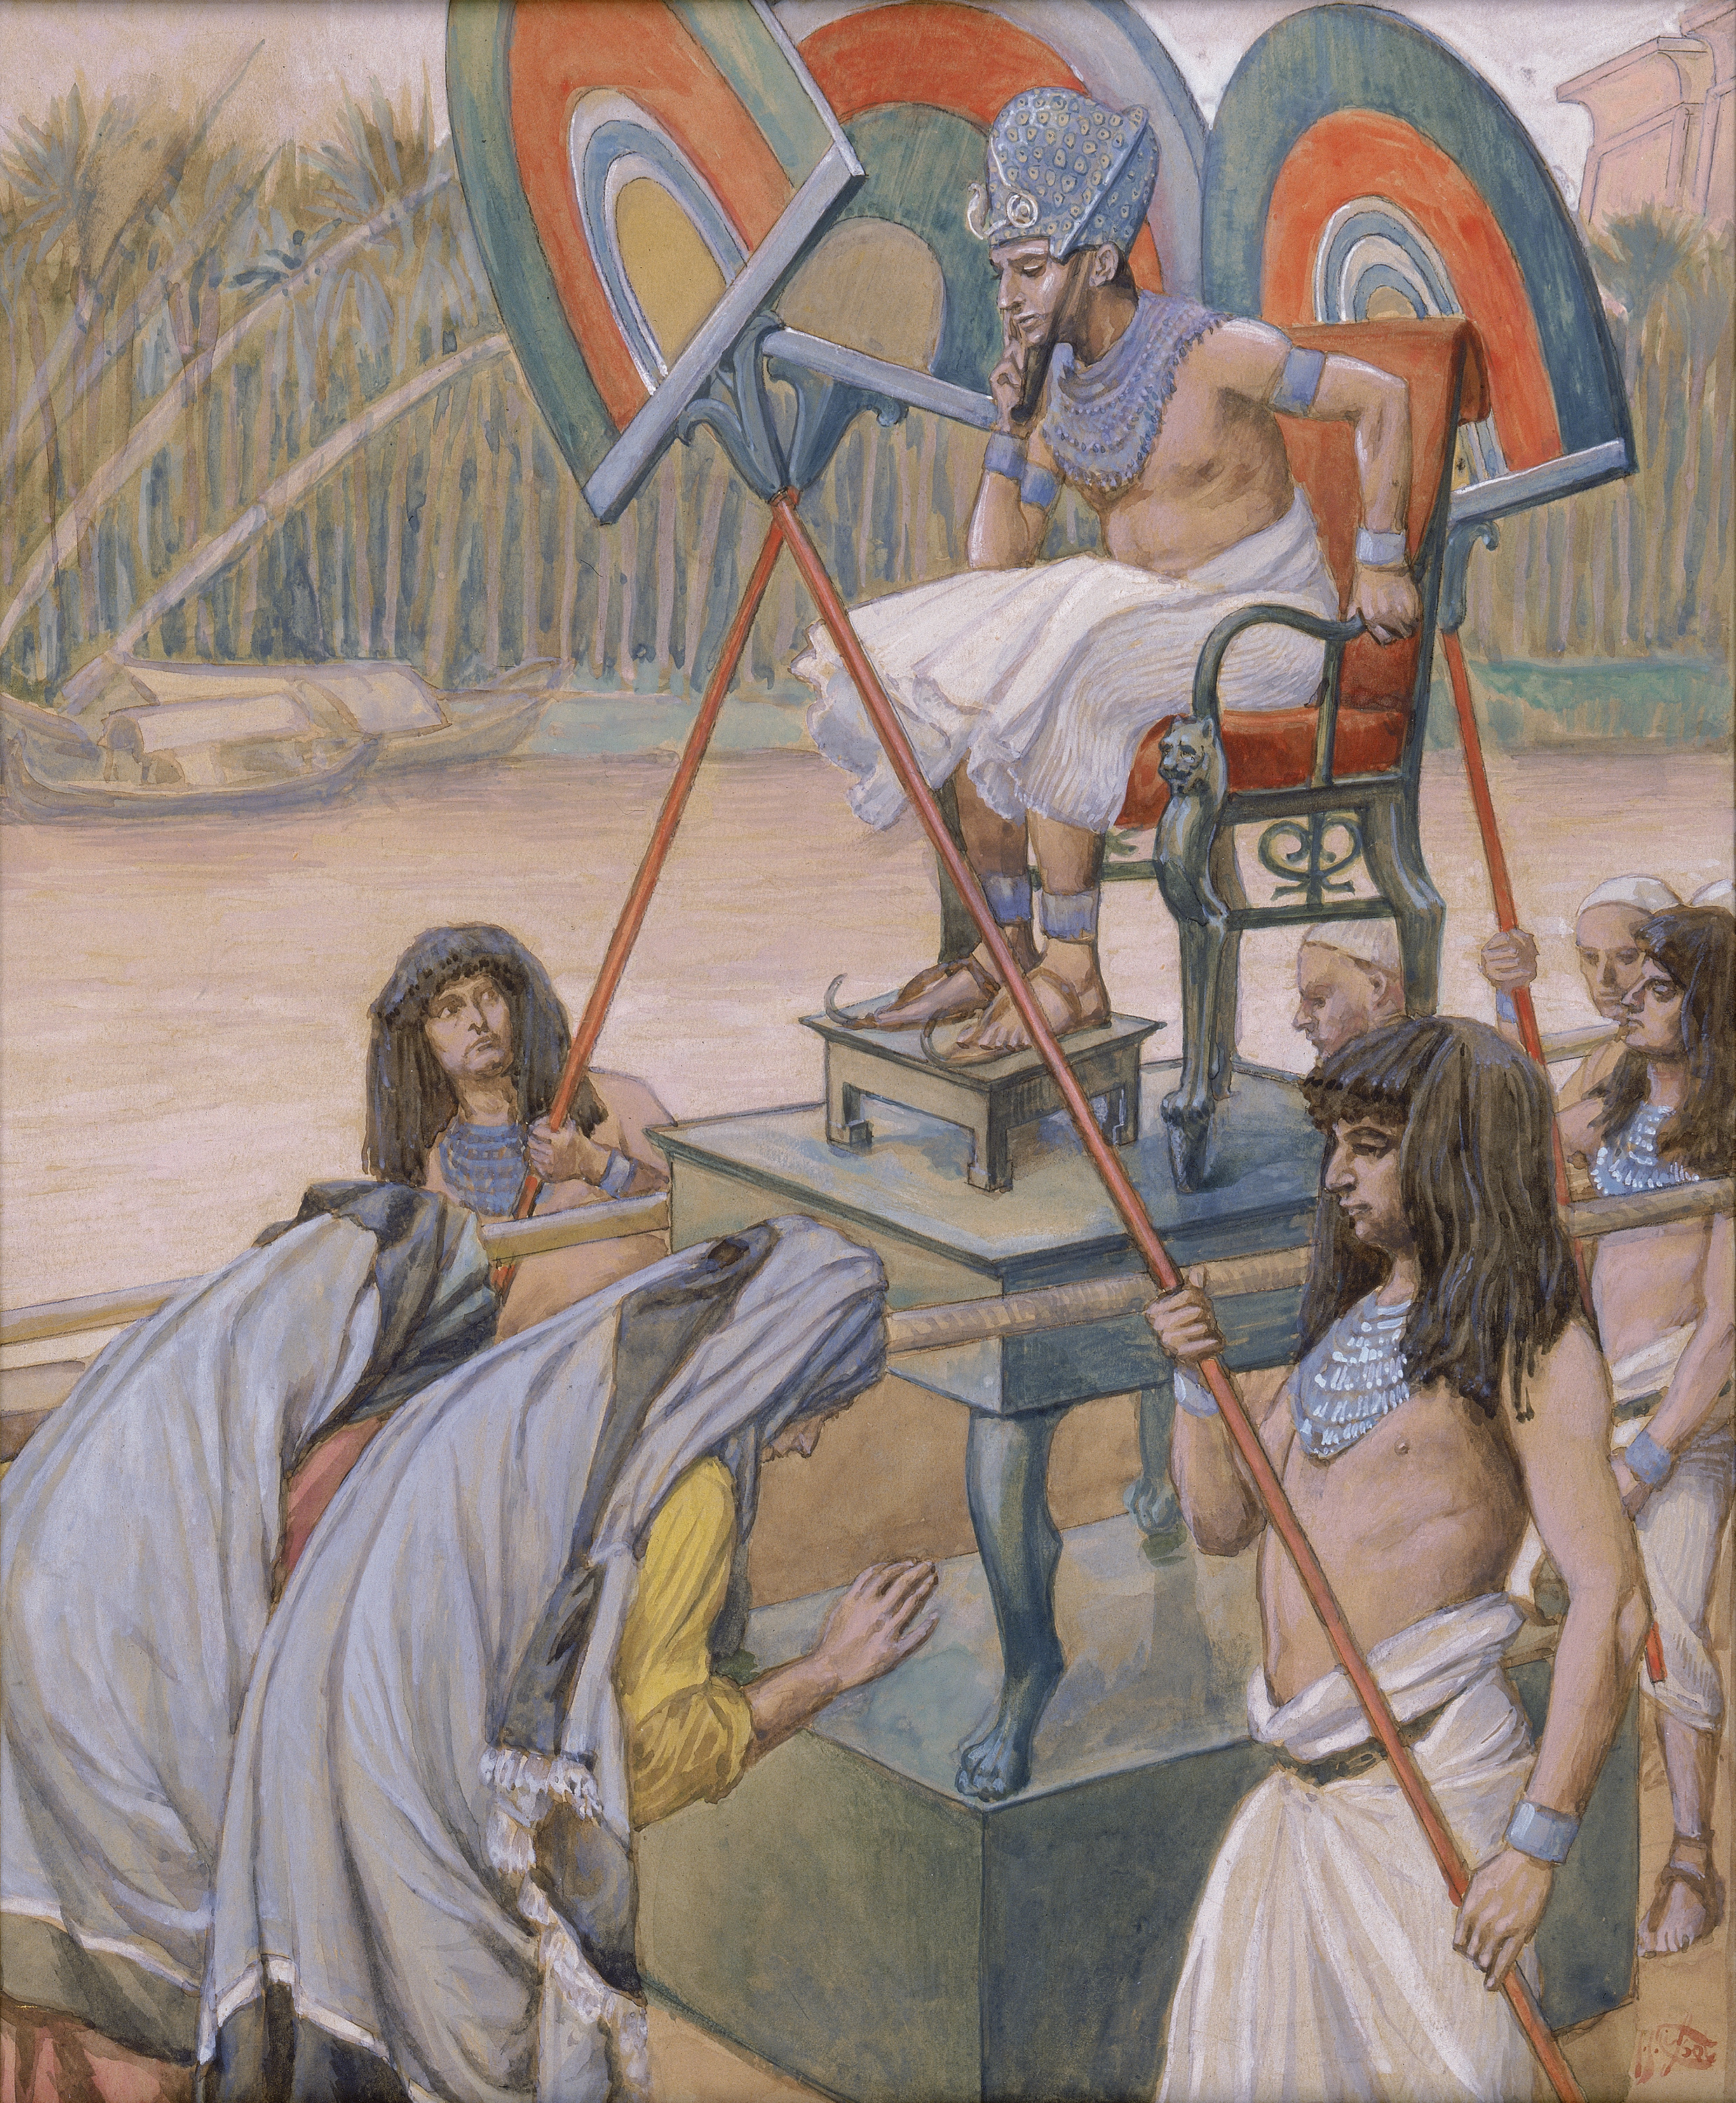
\includegraphics[width=1.3\linewidth]{midwives}}
%    }
%    \caption{\hspace*{-4.5cm}Obstetricēs et Rēx}
%\end{figure}

\titleimg{mw2.jpg}

{\begin{center}\large\bf\underline{Capitulum Primum}\end{center}%}

[In Aegyptō] fīliī Isrāēl crēvērunt, et \marginpar{quasi germinantēs: non vero germinantēs (quia hominēs non germinant) sed vidērī aliquō modō germināre}quasi\marginpar{germināre: emittere germina (ea quae ex plantīs veniunt: semen, fructus, cēt.)} germinantēs \marginpar{multiplicāre: multum facere; augēre}multiplicātī sunt:
ac rōborātī \marginpar{rōborāre: virēs dāre}nimis, implēvērunt terram.

Surrēxit intereā rēx novus super Ægyptum, quī ignōrābat Ioseph.
Et ait ad populum suum: ``Ecce, populus fīliōrum Isrāēl multus, et fortior nōbīs est.
Venīte, \marginpar{{\bf sapienter (adv) <} sapiēns}\marginpar{opprimere: efficere ut aliquis surgere nōn potest}\marginpar{ingruere: cum vi accedere}sapienter opprimāmus eum, nē forte multiplicētur: et sī ingruerit contrā nōs bellum, addātur inimīcīs nostrīs, expugnātisque nōbīs ēgrediātur dē terrā.''

\begin{figure}[h]
    \begin{minipage}[h]{0.5\linewidth}
        \centering
        
\includegraphics{tab}
        \caption{tabernaculum, -ī (n)}
    \end{minipage}%
    \begin{minipage}[h]{0.5\linewidth}
        \vspace*{-0.3cm}
        \centering
        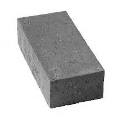
\includegraphics{later}
        \vspace*{-0.425cm}
        \caption{later, lateris (m)}
    \end{minipage}
\end{figure}

Præposuit \marginpar{praeposuit eīs magistrōs operum: dedit magistrīs potestatem super opera fīliōrum Isrāēl}itaque eīs magistrōs operum, ut afflīgerent eōs \marginpar{onus, oneris (n): res quam difficile est portare vel agere. e.g: saccus lapidibus plenus, labor difficilis} oneribus: 
ædificaveruntquē urbēs tabernāculōrum Pharaōnī, Phithom et Ramessēs.
Quantōque opprimēbant eōs, tantō magis multiplicābantur, et crēscēbant: 
ōderantque fīliōs Isrāēl Ægyptiī, et afflīgēbant \marginpar{illūdere: deridēre}illūdentēs eīs,
atque ad \marginpar{{\bf amāritūdo, -inis (f)}\\\hspace{0.5cm} < amārus/a/um $\leftrightarrow$ dulcis, -e}amāritūdinem \marginpar{per-dūcere: trahere}perdūcēbant vītam eōrum operibus dūrīs \marginpar{lutum, -ī(n): terra humida}lutī et lateris, omnīque \marginpar{famulātus, -ūs (m): servitus; conditiō servōrum}famulātū, quō in terræ operibus premēbantur. 
Dīxit autem rēx Ægyptī \marginpar{obstetrix, -īcis(f): femina quae iuvat feminam gravidam parere} obstetrīcibus Hebræōrum, quārum ūna vocābātur Sephora, altera Phua, 
\marginpar{praecipere: imperāre} præcipiēns eīs: ``Quandō obstetrīcābitis Hebræās, et \marginpar{partus, -ūs (m): actus pariendi} partus tempus advēnerit: sī masculus fuerit, interficite eum: sī fēmina, \marginpar{reservāre: servāre, conservāre}reservātē.''

Timuērunt autem obstetrīcēs Deum, \marginpar{praeceptum, -ī: quod praecipitur}\marginpar{nōn fēcērunt iuxtā praeceptum regis: non parent praeceptō rēgis}et nōn fēcērunt iuxtā præceptum rēgis Ægyptī, sed \marginpar{cōnservāre: servāre}cōnservābant \marginpar{mas, maris(m): homo (vel animal) masculinus}marēs. 
Quibus ad sē accersītis, rēx ait: ``Quidnam est hoc quod facere voluistis, ut puerōs servārētis?''

Quæ respondērunt: ``Nōn sunt Hebreæ sīcut Ægyptiæ mulierēs: ipsæ enim obstetrīcandī habent \marginpar{scientia, -ae (f) (< scīre): id quod scītur}scientiam, et priusquam veniāmus ad eās, pariunt.''

Bene ergō fēcit Deus obstetrīcibus: et crēvit populus, \marginpar{cōnfortāre: fortem facere, consolārī}cōnfortātusque est nimis.
Et quia timuērunt obstetrīcēs Deum, ædificāvit eīs domōs.
Præcēpit ergō Pharaō omnī populō suō, dīcēns: ``Quidquid masculīnī sexūs nātum fuerit, in flūmen prōiicite: quidquid fēminīnī, reservātē.''

\chapter{}

\titleimg{baby2.jpg}

\mktitle{Capitulum Secundum}
\thispagestyle{empty}

\vnum{1}Ēgressus est post hæc vir dē domō Levī: et accēpit uxōrem \mpp{stirps, stirpis (m/f):}{e.g, frater matris est `stirpis meae', filia sororis patris quoque est `stirpis meae'. Quisquis ex familiā meā est, `stirpis meae' vocatur}stirpis suæ.
\vnum{2}Quæ \mpp{concipere:}{femina quae concipit efficit ut infans in eā incipit crescere}concēpit, et peperit fīlium: et vidēns eum \mpp{ēlegāns =}{pulcher}ēlegantem, abscondit tribus mēnsibus.
\mpp{scirpeus/a/um:}{ex scirpīs factus}
\mpp{līnere:}{ponere rem mollem premendō ac tergendō}
\mpp{bitūmen, -inis (n):}{māteria mollis atque ātra in terrā inventa quae pōnitur in rēbus nē aqua īnfluere possit}


\begin{figure}[hp]
    \begin{minipage}[hbp]{0.5\linewidth}
        \centering
        \includegraphics{basket}
        \caption{fiscella, -ae (f)}
    \end{minipage}%
    \begin{minipage}[hbp]{0.5\linewidth}
        \centering
        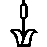
\includegraphics{brush}
        \caption{scirpus, -ī (m)}
    \end{minipage}
\end{figure}

\vnum{3}Cumque iam cēlāre nōn posset, sūmpsit fiscellam scirpeam,
et līnīvit eam bitūmine ac \mpp{pix, picis (f):}{māteria bitūminī similis mollis atque ātra ex parte arboris facta}pice:
posuitque intus īnfantulum, et exposuit eum in \mpp{cārex, cāricis (f):}{herba acuta et durissima}\mpp{cārectum, -ī (n):}{locus caricibus plenus}cārectō \mpp{rīpa, -ae (f):}{terra tangēns flumen}
rīpæ flūminis,
\vnum{4}stante procul sorōre eius, et \mpp{cōnsīderāns ēventum reī:}{exspectans ut videat quid futurum sit}
cōnsīderante ēventum reī.
\vnum{5}Ecce autem dēscendēbat fīlia Pharaōnis ut lavārētur in flūmine.\mpp{crepīdo, -inis (f):}{ripa fluminis lapidibus strata}\mpp{alveus, -ī (m):}{fossa per quam fluvius fluit} Et puellæ eius \mpp{gradī:}{gradum facere, ambulāre}gradiēbantur per crepīdinem alveī.
\mpp{papyrio, -ōnis (m):}{locus multīs cum papyrīs}Quæ cum vīdisset fiscellam in papȳriōne,
mīsit ūnam ē \mpp{famula, -ae (f):}{ancilla}famulābus suīs: et allātam \vnum{6}aperiēns,
cernēnsque in eā parvulum vāgientem,
\mpp{miserta (+ gen.):}{tristis propter aliquem miserum}miserta eius, ait: ``Dē īnfantibus Hebræōrum est hic.''

\vnum{7}Cui soror puerī: ``Vīs,'' inquit, ``ut vādam, et vōcem tibi mulierem Hebræam,
quæ \mpp{nūtrīre:}{dāre lac}nūtrīre possit \mpp{īnfantulus/a/um:}{parvus īnfans}īnfantulum?''\mimg{papyrus}{papyrus, -ī (m/f)}

\vnum{8}Respondit: ``Vāde.''

Perrēxit puella et vocāvit mātrem suam.
\vnum{9}Ad quam locūta fīlia Pharaōnis: ``Accipe,'' ait, ``puerum istum, et nūtrī mihi: ego dabō tibi mercēdem tuam.''

\mpp{suscipere:}{sumere, capere}Suscēpit mulier, et nūtrīvit puerum: \mpp{adultus/a/um:}{iam vir/femina, non puer/puella}adultumque trādidit fīliæ Pharaōnis. 
\mpp{adoptāre:}{qui adoptat aliquem facit eum filium vel filiam suam}\vnum{10}Quem illa adoptāvit in locum fīliī,
vocāvitque nōmen eius Moysēs, dīcēns: ``Quia dē aquā tulī eum.''

\vnum{11}In diēbus illīs postquam crēverat Moysēs, ēgressus est ad frātrēs suōs:
\mpp{percutere:}{pulsare, afficere, et quasi vulnerare dolore}vīditque afflīctiōnem eōrum et virum Ægyptium percutientem quemdam dē Hebræīs frātribus suīs.
\vnum{12}Cumque circumspexisset hūc atque illūc,
et nūllum adesse vīdisset,
\mimg{sabulum}{sabulum, -ī (n)}\mpp{abscondere:}{rem in aliquo loco ponere ut celetur}
percussum Ægyptium abscondit sabulō.
\mpp{rixāre:}{certāre}

\vnum{13}Et ēgressus diē alterō cōnspexit duōs Hebræōs rixantēs:
dīxitque eī quī faciēbat iniūriam: ``Quārē percutis proximum tuum?''

\mpp{prīnceps, prīncipis (m):}{rex; dux}\vnum{14}Quī respondit: ``Quis tē cōnstituit prīncipem et \mimg{judge_small}{\hspace*{0.75cm}iūdex, iūdicis (m/f)}iūdicem super nōs?
Num occīdere mē tū vīs, sīcut heri occīdistī Ægyptium?''

\mpp{palam}{$\leftrightarrow$ occulte}Timuit Moysēs, et ait: ``Quōmodo palam factum est verbum istud?''

\vnum{15}Audīvitque Pharaō sermōnem hunc, et quærēbat occīdere Moysēn:
quī fugiēns dē cōnspectū eius, morātus est in terrā Madiān,
\mimg{puteus.png}{puteus, -ī (m)}et sēdit iuxtā puteum.
\vnum{16}Erant autem sacerdōtī Madian septem fīliæ,
quæ vēnērunt ad \mpp{haurīre:}{sumere ex loco ubi aqua est}hauriendam aquam:
\mpp{adaquāre:}{aquam dāre}et implētīs \mpp{canālis, -is (m/f):}{rēs in quam aqua funditur ut animal bibat}canālibus adaquāre cupiēbant gregēs patris suī.
\mpp{supervēnīre:}{subitō adesse nocendī causā}\mpp{supervēnēre =}{supervēnērunt}\vnum{17}Supervēnēre pāstōrēs, et ēiēcērunt eās:
surrēxitque Moysēs, et dēfēnsīs puellīs, adaquāvit ovēs eārum. 
\vnum{18}Quæ cum revertissent ad Raguel patrem suum, dīxit ad eās:
\mpp{vēlox, -ōcis:}{celer}``Cūr vēlōcius vēnistis solitō?''

\vnum{19}Respondērunt: ``Vir Ægyptius līberāvit nōs dē manū pāstōrum:
\mpp{īnsuper:}{praeterea}īnsuper et hausit aquam nōbīscum, \mpp{pōtus, -ūs (m):}{pōtiō}pōtumque dedit ovibus.''

\vnum{20}At ille: ``Ubi est?'' inquit: ``Quārē dīmīsistis hominem? Vocātē eum ut \mpp{comedere:}{totum ēsse; ēsse}comedat pānem.''

\vnum{21}Iūrāvit ergō Moysēs quod habitāret cum eō.
Accēpitque Sephoram fīliam eius uxōrem:
\vnum{22}Quæ peperit eī fīlium, quem vocāvit Gersam, dīcēns:
\mpp{advena, -ae (m)}{quī nōn est cīvis, qui ab aliō locō venit}``Advena fuī in \mpp{terra aliēna:}{terra ubi is nōn natus est}terrā aliēnā.''

Alterum vērō peperit, quem vocāvit Eliezer, dīcēns:
\mpp{adiūtor, -ōris (m):}{qui adiuvat}``Deus enim patris meī adiūtor meus ēripuit mē dē manū Pharaōnis.''

\vnum{23}Post multum vērō tempore mortuus est rēx Ægyptī:
\mpp{ingemīscere:}{dolēre}et ingemīscentēs fīliī Isrāēl
propter opera vōciferātī sunt:
\mpp{vōciferātus/a/um $<$ vōciferārī:}{valde exclamāre}
ascenditque clāmor eōrum ad Deum ab operibus.
\mpp{gemitus, -ūs (m):}{sonus atque actus dolendī}\vnum{24}Et audīvit gemitum eōrum,
\mpp{pangō, pangere, pepigisse, pactum:}{constituere, statuere}ac \mpp{recordor, -ārī, -ātus sum:}{meminisse}recordātus est fœderis quod pepigit cum Abraham, Isaac et Iācōb.
\mpp{respicere:}{aspicere iuvandī causā}\vnum{25}Et respexit Dominus fīliōs Isrāēl et cognōvit eōs.

\chapter{}

\titleimg{bush2.jpg}
\thispagestyle{empty}

\mktitle{Capitulum Tertium}
\vspace*{-0.75cm}
Moysēs autem pāscēbat ovēs Iethrō \mpp{socer, socerī:}{pater uxōris vel pater marītī}suī sacerdōtis Madian:
\mpp{mināre:}{cōgere animālia}cumque mināsset gregem ad \mpp{interiōr, -ōris (adj.):}{magis intus}interiōra \mpp{dēserta, -ōrum (n):}{locus ubi paene nihil est; locus sine imbre et aquā}dēsertī,
venit ad montem Deī Horeb.
\mpp{rubus, -ī (m):}{quaedam herba}
Appāruitque eī Dominus in flammā ignis dē mediō rubī:
et vidēbat quod rubus \mpp{ārdēre:}{habēre ignem in sē}ārdēret, et nōn \mpp{combūrere:}{igne perdere}combūrerētur.
Dīxit ergō Moysēs: \mpp{vādere:}{īre, ambulāre}``Vādam, et vidēbō \mpp{vīsiō, -ōnis (f):}{quod vīsum est; āctus videndī}vīsiōnem hanc magnam, quārē nōn combūrātur rubus.''

Cernēns autem Dominus quod pergeret ad videndum,
vocāvit eum dē mediō rubī, et ait: ``Moysēs, Moysēs.''

Quī respondit: ``Adsum.''

At ille: ``Nē \mpp{appropiāre =}{adīre}appropiēs,'' inquit, ``hūc: solve \mpp{calceāmentum:}{quod pedī induitur}calceāmentum dē pedibus tuīs: locus enim
in quō stās \mpp{terra sāncta:}{terra deō cōnstitūta}terra sāncta est.'' 

Et ait: ``Ego sum Deus patris tuī, Deus Abraham, Deus Isaac et Deus Iācōb.''

Abscondit Moysēs faciem suam: nōn enim audēbat aspicere contrā Deum.

Cui ait Dominus: ``Vīdī \mpp{afflīctiō, -ōnis (f):}{rēs quae nocet vel valde non placet}afflīctiōnem populī meī in Ægyptō,
et clāmōrem eius audīvī propter \mpp{duritia, -ae (f) $<$}{durus/a/um}dūritiam eōrum quī \mpp{prae-esse:}{esse prae alios; dux esse}præsunt operibus:
et sciēns dolōrem eius, dēscendī ut libērem eum dē manibus Ægyptiōrum,
et ēdūcam dē terrā illā in terram bonam, et \mpp{spatiōsus/a/um:}{magnus}spatiōsam,
in terram quæ fluit lacte et melle,
\mpp{loca =}{locī (nom. pl.)} ad loca Chananæī et Hethæī, et Amorrhæī, et Pherezæī, et Hevæī, et Iebusæī.
Clāmor ergō fīliōrum Isrāēl venit ad mē: vīdīque afflīctiōnem eōrum,
qua ab Ægyptiīs \mpp{opprimere:}{efficere ut aliquis surgere nōn possit}opprimuntur.
Sed vēnī, et mittam tē ad Pharaōnem,
ut ēducās populum meum, fīliōs Isrāēl, dē Ægyptō.''

Dīxitque Moysēs ad Deum: ``Quis sum ego ut vādam ad Pharaōnem,
et ēdūcam fīliōs Isrāēl dē Ægyptō?''

Quī dīxit eī: ``Ego erō tēcum: et hoc habēbis signum,
quod mīserim tē: cum ēdūxerīs populum meum dē Ægyptō,
immolābis Deō super montem istum.''

Ait Moysēs ad Deum: ``Ecce ego vādam ad fīliōs Isrāēl,
et dīcam eīs: Deus patrum vestrōrum mīsit mē ad vōs.
Sī dīxerint mihi: `Quod est nōmen eius?' quid dīcam eīs?''

Dīxit Deus ad Moysēn: ``EGO SUM QUĪ SUM.'' Ait: ``Sīc dīcēs fīliīs Isrāēl: `QUĪ EST mīsit mē ad vōs.' ''

Dīxitque iterum Deus ad Moysēn: ``Hæc dīcēs fīliīs Isrāēl:
Dominus Deus patrum vestrōrum, Deus Abraham, Deus Isaac et Deus Iācōb,
\mpp{in æternum:}{semper} mīsit mē ad vōs: hoc nōmen mihi est in æternum,
\mpp{memoriāle, -is (n):}{id quod memorandum est}et hoc memoriāle meum in generātiōnem et generātiōnem.''

``Vāde, et \mpp{congregāre:}{in unum locum cōgere vel ferre vel ducere}, congregā \mpp{seniōr, -ōris (adj):}{magis senex; hīc seniōrēs virī, id est, principēs}seniōrēs Isrāēl,
et dīcēs ad eōs: Dominus Deus patrum vestrōrum appāruit mihi,
Deus Abraham, Deus Isaac et Deus Iācōb,
\mpp{vīsitāre:}{vīsum īre}dīcēns: Vīsitāns vīsitāvī vōs: et vīdī omnia quæ accidērunt vōbīs in Ægyptō.
Et dīxī ut ēdūcam vōs dē \mpp{afflīctiō, -ōnis (f):}{rēs quae nocet vel valde non placet}afflīctiōne Ægyptī in terram Chananæī,
et Hethæī, et Amorrhæī, et Pherezæī, et Hevæī, et Iebusæī,
ad terram fluentem lacte et melle.''

``Et audient vōcem tuam: ingrediērisque tū,
et seniōrēs Isrāēl, ad rēgem Ægyptī, et dīcēs ad eum:
Dominus Deus Hebræōrum vocāvit nōs:
ībimus viam trium diērum in \mpp{sōlitūdo, -inis ($<$ solus/a/um):}{deserta; locus ubi nemo vel unus habitat}sōlitūdinem,
\mpp{immolāre:}{sacrificium facere}ut immolēmus Dominō Deō nostrō.''

``Sed ego sciō quod nōn dīmittet vōs rēx Ægyptī
ut eātis nisi per manum validam.
Extendam enim manum meam, et percutiam Ægyptum
in cūnctīs mīrābilibus meīs, 
quæ factūrus sum in mediō eōrum:
post hæc dīmittet vōs.
Dabōque grātiam populō huic cōram Ægyptiīs:
\mpp{vacuuus/a/um:}{sine rēbus (cibō, vestimentīs, pecuniā)}et cum ēgrediēminī, nōn exībitis vacuī:
\mpp{vīcīnus/a:}{qui prope habitat}sed postulābit mulier ā vīcīnā suā
et ab hospitā suā, vāsa argentea et aurea, ac vestēs:
\mpp{spoliāre:}{capere rēs aliōrum hominum}pōnētisque eās super fīliōs et fīliās vestrās, et spoliābitis Ægyptum.''

\chapter{}

\titleimg{inn.png}

{\begin{center}\large\bf\underline{Capitulum Quartum}\end{center}}
\vspace*{-1.0cm}

Respondēns Moysēs ait: ``Nōn crēdent mihi, neque audient vōcem meam, sed dīcent:
Nōn appāruit tibi Dominus.''

Dīxit ergō ad eum: ``Quid est quod tenēs in manū tuā?''

Respondit: ``Virga.''

\marginpar{prōiicere: procul iacere; abiicere} Dīxitque Dominus: ``Prōiice eam in terram.''

Prōiēcit, et versa est in colubrum, ita ut fugeret \marginpar{coluber, -brī (m): serpens}Moysēs. 

Dīxitque Dominus: ``Extende manum tuam, et apprehende caudam eius.''

Extendit, et tenuit, versaque est in virgam.
``Ut crēdant,'' inquit, ``quod appāruerit tibi Dominus Deus patrum suōrum,
Deus Abraham, Deus Isaac et Deus Iācōb.''

Dīxitque Dominus rūrsum: ``Mitte manum tuam in sinum tuum.''

\marginpar{{\bf leprōsus/a/um $<$ leprae, -ārum (f)}: morbus qui cutem (exterior pars hominis) deformat}
\marginpar{īnstar + gen: sicut}Quam cum mīsisset in sinum, prōtulit leprōsam īnstar nivis.
``Retrahe,'' ait, ``manum tuam in sinum tuum.''

Retrāxit, et prōtulit iterum,
et erat similis carnī reliquæ.
``Sī nōn crēdiderint,'' inquit, ``tibi, neque audierint
sermōnem signī priōris, crēdent verbō signī sequentis. 
Quod sī nec duōbus quidem hīs signīs crēdiderint,
neque audierint vōcem tuam: sūme aquam flūminis,
\marginpar{āridus/a/um: sine aquā}et effunde eam super āridam, et quidquid hauserīs dē fluviō,
vertētur in sanguinem.''

\marginpar{nūdiustertius: ante duōs diēs}
Ait Moysēs: ``Obsecrō, Domine, nōn sum ēloquēns ab heri et
\marginpar{{\bf ex quō} (tempore)}nūdiustertius: et ex quō locūtus es ad servum tuum,
impedītiōris et tardiōris linguæ sum.''

Dīxit Dominus ad eum: ``Quis fēcit os hominis?
\marginpar{fabricatus/a/um: confectus}
\marginpar{mūtus/a/um: loquī non potest}
\marginpar{surdus/a/um: audīre non potest}
aut quis fabricātus est mūtum et surdum,
\marginpar{caecus/a/um: vidēre non potest}videntem et cæcum? nōnne ego?
Perge, igitur, et ego erō in ōre tuō:
docēbōque tē quid loquāris.''

\marginpar{obsecrāre: orāre, precārī}At ille: ``Obsecrō, inquit, Domine,
mitte quem missūrus es.''

Īrātus Dominus in Moysēn, ait: ``Aarōn frāter tuus Lēvītēs,
sciō quod ēloquēns sit: ecce ipse ēgreditur in occursum tuum,
vidēnsque tē lætābitur corde.
Loquere ad eum, et pōne verba mea in ōre eius:
et ego erō in ōre tuō, et in ōre illīus,
et ostendam vōbīs quid agere dēbeātis.
Ipse loquētur prō tē ad populum,
et erit os tuum:
tū autem eris eī in hīs quæ ad Deum pertinent.
Virgam quoque hanc sūme in manū tuā,
in quā factūrus es signa.

\marginpar{socer, socerī (m): pater uxōris}Abiit Moysēs, et reversus est ad Iethrō socerum suum,
dīxitque eī: ``Vādam et revertar ad frātrēs meōs in Ægyptum,
ut videam sī adhūc vīvant.''

Cui ait Iethrō: ``Vāde in pāce.''

Dīxit ergō Dominus ad Moysēn in Madiān: ``Vāde, et revertere in Ægyptum,
mortuī sunt enim omnēs quī quærēbant animam tuam.''

\begin{figure}[hbp]
        \centering
        \setlength{\fboxsep}{0pt}
        \fbox{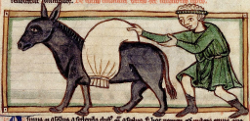
\includegraphics{asinus}}
        \caption{asinus, -ī (m)}
\end{figure}
Tulit ergō Moysēs uxōrem suam, et fīliōs suōs,
et imposuit eōs super asinum: reversusque est in Ægyptum,
portāns virgam Deī in manū suā. Dīxitque eī Dominus revertentī
in Ægyptum: ``Vidē ut omnia ostenta quæ posuī in manū tuā
\marginpar{indūrāre: durum facere}faciās cōram Pharaōne: ego indūrābō cor eius,
et nōn dīmittet populum. Dīcēsque ad eum: Hæc
\marginpar{prīmōgenitus: natū maior}dīcit Dominus: Fīlius meus prīmōgenitus Isrāēl.
Dīxī tibi: Dīmitte fīlium meum ut serviat mihi;
et nōluistī dīmittere eum:
ecce ego interficiam fīlium tuum prīmōgenitum.''

\marginpar{dīversōrium, -ī (n): aedificium in quō hominēs in itinere possunt dormīre}\marginpar{petra, -ae (f): lapis}Cumque esset in itinere, in dīversōriō
occurrit eī Dominus, et volēbat occīdere eum. 
\marginpar{idcircō: proptereā, ideō}Tulit idcircō Sephora acūtissimam petram,
\marginpar{praepūtium, -ī (n): illa pars puerī quae circumcīditur}et circumcīdit præpūtium fīliī suī, tetigitque pedēs ejus,
\marginpar{spōnsus/a: quī mox alicui maritus vel uxor erit}et ait: ``Spōnsus sanguinum tū mihi es.''
Et dīmīsit eum postquam dīxerat: ``Spōnsus sanguinum ob circumcīsiōnem.''

Dīxit autem Dominus ad Aarōn: ``Vāde in occursum Moȳsī
in dēsertum.'' 

Quī perrēxit obviam eī in montem Deī, et ōsculātus est eum.
Nārrāvitque Moysēs Aarōn omnia verba Dominī quibus miserat eum,
et signa quæ mandāverat. Vēnēruntque simul, et congregāvērunt
cūnctōs seniōrēs fīliōrum Isrāēl.
Locūtusque est Aarōn omnia verba quæ dīxerat Dominus ad Moysēn: et
fēcit signa cōram populō, et crēdidit populus.
Audiēruntque quod vīsitāsset Dominus fīliōs Isrāēl,
\marginpar{prōnus/a/um: iacēns in pectore}et respexisset afflīctiōnem illōrum: et prōnī adōrāvērunt.

\chapter{}
\titleimg{bricks.jpg}
\mktitle{Capitulum Quintum}
\thispagestyle{empty}

Post hæc \mpp{ingredī:}{intus īre}ingressī sunt Moysēs
et Aarōn, et dīxērunt Pharaōnī: ``Hæc dīcit Dominus Deus
Isrāēl: Dīmitte populum meum ut
\mpp{sacrificāre}{animal interficere vel rem offerre ut placeat deō}sacrificet mihi in dēsertō.''

At ille respondit: ``Quis est
Dominus, ut audiam vōcem eius, et dīmittam Isrāēl? Nesciō
Dominum, et Isrāēl nōn dīmittam.''

Dīxēruntque: ``Deus
Hebræōrum vocāvit nōs, ut eāmus viam trium diērum in
\mpp{sōlitūdō:}{deserta; locus ubi nemo vel unus habitat}sōlitūdinem, et
sacrificēmus Dominō Deō nostrō: nē forte accidat nōbīs
\mpp{pestis, -is (f):}{aliquid corporī malum: e.g, aeger fiērī}pestis aut
gladius.''

Ait ad eōs rēx Ægyptī: ``Quārē
Moysēs et Aarōn \mpp{sollicitāre:}{allicere}sollicitātis populum ab
operibus suīs? Īte ad \mpp{onus, oneris (n):}{res quae difficile est portare vel agere. e.g: saccus lapidibus plenus, labor difficilis}onera vestra.''

Dīxitque
Pharaō: ``Multus est populus terræ: vidētis quod turba
\mpp{succrēscere (sub + crēscere):}{ab īmō crēscere}succrēverit: quantō magis sī dederītis eīs
\mpp{requiēs, requieī (f):}{tempus quō homō non laborāt}requiem ab operibus?'' 

\kimg{palea}{paleam colligentes}

Præcēpit \mpp{praecipere:}{imperāre}ergō in diē illō
\mpp{praefectus, -ī (m):}{homo qui alicuī reī vel negotiō praepositus est}præfectīs operum et \mpp{exāctōr, -ī:}{quī facit ut opera perficiantur}exāctōribus populī,
dīcēns:  ``\mpp{nēquāquam:}{minimē, nullō modō}Nēquā\-quam ultrā dabitis paleās
populō ad cōnficiendōs laterēs, sīcut prius: sed ipsī \mpp{vadere:}{īre, ambulāre}vadant, et colligant \mpp{stipula, ae}{media ac longa pars herbae
ex quā aliae partēs extendunt}stipulās. 
Et \mpp{mēnsūra:}{e.g, si praefectus dicit ``pone centum laterēs in hōc
vase,'' centum laterēs est {\it mēnsūra} laterum}mēnsūram laterum, quam prius faciēbant, impōnētis super eōs, nec
minuētis quidquam: \mpp{vacāre:}{sine negotiīs esse}vacant enim, et
\mpp{idcirco:}{propterea, ideo}idcircō \mpp{vociferatus:}{valde exclamare}vōciferantur, dīcentēs: Eāmus, et sacrificēmus
Deō nostrō.  \mpp{opprimere:}{efficere ut aliquis surgere non possit}Opprimantur operibus, et \mpp{explēre:}{perficere}expleant ea: ut nōn
\mpp{acquiescere:}{fidem habere}acquiēscant verbīs
\mpp{mendāx, -ācis (adj):}{mentiēns}mendācibus.''

Igitur ēgressī præfectī
operum et exāctōrēs ad populum dīxērunt: ``Sīc dīcit
Pharaō: Nōn dō vōbīs paleās:  Īte, et
colligite \mpp{sīcubi:}{sī in aliquō locō}sīcubi invenīre poteritis, nec
minuētur quidquam dē opere vestrō.''

Dispersusque \mpp{dispergō, dispergere, dispersī, dispersus:}{in multās et variās partēs vel loca spargere}est
populus per omnem terram Ægyptī ad colligendās
paleās.

Præfectī quoque operum
\mpp{īnstāre:}{in vel super aliquā rē stāre}īnstābant, dīcentēs: ``Complētē opus vestrum
\mpp{quotīdiē:}{cotīdiē}quotīdiē, ut prius facere solēbātis quandō dabantur vōbīs
paleæ.''  

\mimg{flagellum}{flagellum, -ī (n)}
Flagellātīque \mpp{flagellāre:}{flagellīs pulsāre}sunt quī præerant
operibus fīliōrum Isrāēl, ab exāctōribus
Pharaōnis, dīcentibus: ``Quārē nōn implētis mēnsūram
laterum sīcut prius, nec heri, nec hodiē?''

Vēnēruntque præpositī
fīliōrum Isrāēl, et \mpp{vociferatus:}{valde exclamare}vōciferātī sunt ad Pharaōnem dīcentēs: ``Cūr ita
agis contrā servōs tuōs?  Paleæ nōn dantur nōbīs, et
laterēs \mpp{similiter (adv)}{$<$ similis}similiter imperantur:
\mpp{ēn:}{ecce}ēn
\mpp{famulus, -ī (m)}{servus}famulī
tuī flagellīs cædimur, et iniūstē agitur contrā populum
tuum.''

Quī ait: ``Vacātis ōtiō, et
\mpp{idcirco:}{propterea, ideo}idcircō dīcitis: Eāmus, et
sacrificēmus Dominō.  Īte ergō, et operāminī:
paleæ nōn dabuntur vōbīs, et reddētis
\mpp{cōnsuētus/a/um:}{e.g, si cotidue quinque nummos tibi do, hic numerus
nummōrum est numerus {\it cōnsuētus} inter nōs}cōnsuētum numerum laterum.''

Vidēbantque sē præpositī
fīliōrum Isrāēl in malō, eō quod dīcerētur eīs: Nōn
minuētur quidquam dē lateribus per singulōs diēs.  Occurrēruntque Moȳsī
et Aarōn, quī stābant ex adversō, ēgredientibus ā Pharaōne:
et dīxērunt ad eōs: ``Videat Dominus et \mimg{judge_small}{iudex, iudicis (m/f)}\mpp{iudicāre:}{quod iudex tradit}iūdicet,
quoniam \mpp{foetēre:}{emittere malum odorem}fœtēre fēcistis \mpp{odōr, odōris (m)}{quod nasus sentit}odōrem nostrum cōram
Pharaōne et servīs eius, et \mpp{praebeō, praebēre, praebuī, praebitum:}{offerre}præbuistis eī
gladium, ut occīderet nōs.''

Reversusque est Moysēs ad
Dominum, et ait: ``Domine, cūr \mpp{affligere:}{perdere}afflīxistī populum
is\-tum? Quārē mīsistī mē?  Ex eō enim quō \mpp{ingredī:}{intus īre}ingressus sum ad Pharaōnem ut loquerer in nōmine tuō,
\mpp{affligere:}{perdere}afflīxit populum tuum: et nōn līberāstī eōs.''


\chapter{}
\titleimg{cap6.png}
\mktitle{Capitulum Sextum}
\thispagestyle{empty}
Dīxitque Dominus ad \mpp{Moysēn (acc)}{}Moysēn: ``Nunc vidēbis quæ factūrus
sim \mpp{Pharaō, -ōnis (m):}{rēx Aegyptōrum}Pharaōnī: per manum enim fortem dīmittet eōs, et in
manū \mpp{rōbustus/a/um:}{durus, rigidus, valens}rōbustā ēiiciet illōs dē
terrā suā.''

Locūtusque est
Dominus ad Moysēn dīcēns: ``Ego Dominus quī appāruī
Abraham, Isaac et Iācōb in Deō \mpp{omnipotens:}{habens omnem potestatem}omnipotente:
et nōmen meum \mpp{Adonaī:}{vocabulum Hebraicum significans `dominī'}Adonaī
nōn \mpp{indicāre:}{ostendere, monstrāre}indicāvī eīs. 
\mpp{pangō, pangere, pepigisse, pactum:}{constituere, statuere}Pepigīque fœdus cum eīs, ut darem eīs terram
Chanaan, terram \mpp{peregrīnātiō, -ōnis (f)}{ < peregrinārī: iter facere
per aliēna loca, patria procul abīre}peregrīnātiōnis eōrum, in
quā fuērunt advenæ.  Ego audīvī \mpp{gemitus:}{sonus atque actus
dolendi}gemitum fīliōrum Isrāēl, quō Ægyptiī
\mpp{opprimere:}{efficere ut aliquis surgere non possit}oppressērunt\linebreak eōs:
et \mpp{recordor, -ārī, -ātus sum:}{meminisse}recordātus sum \mpp{pactum, -ī (n):}{quod inter aliquōs convenit}pactī meī.  Ideō dīc
fīliīs Isrāēl: Ego Dominus quī ēdūcam vōs dē
\mpp{ergastulum, -ī:}{carcer rusticus}ergastulō Ægyptiōrum, et ēruam dē servitūte, ac redimam in
\mpp{brāchium}{ = bracchium}brāchiō \mpp{excelsus/a/um:}{altus}excelsō et
\mpp{iūdicium, -ī}{quod iudex tradit}\mimg{judge_small}{iudex, iudicis (m/f)}iūdiciīs
magnīs.  Et assūmam vōs mihi in populum, et erō vester Deus: et sciētis
quod ego sum Dominus Deus vester quī ēdūxerim vōs dē
ergastulō Ægyptiōrum,  et indūxerim in terram, super quam
levāvī manum meam ut darem eam Abraham, Isaac et Iācōb:
dabōque illam vōbīs possidendam. Ego Dominus.''

Nārrāvit ergō
Moysēs omnia fīliīs Isrāēl, quī nōn
\mpp{acquiescere:}{fidem habere}acquiēvērunt eī propter \mpp{angustia, -ae (f):}{locus nōn latus}angustiam
\mpp{spīritus, -ūs (m):}{animus}spīritūs et opus dūrissimum.  

Locūtusque est Dominus ad
Moysēn, dīcēns:  ``\mpp{ingredī:}{intus īre}Ingredere, et
loquere ad Pharaōnem rēgem Ægyptī, ut dīmittat fīliōs
Isrāēl dē terrā suā.''

Respondit Moysēs
cōram Dominō: ``Ecce fīliī Isrāēl nōn audiunt mē: et
quōmodo audiet Pharaō, \mpp{præsertim:}{praecipue}præsertim cum
\mpp{labium:}{labrum}
\mpp{``incircumcīsus labiīs'':}{fortasse homo labiīs
``incircumcīsus'' non iam ad loquendum deō constitutus est, sicut vir
incircumcīsus non iam ad deum serviendum constitutus est}incircumcīs\-us sim labiīs?''

Locūtusque est Dominus ad
Moysēn et Aarōn, et dēdit \mpp{mandātum, -ī (n)}{id quod imperatum vel traditum est}mandātum ad
fīliōs Isrāēl, et ad Pharaōnem rēgem Ægyptī
ut ēdūcerent fīliōs Isrāēl dē terrā Ægyptī.

%Dīxitque Dominus ad Moysēn: ``Nunc vidēbis quæ factūrus
%sim Pharaōnī: per manum enim fortem dīmittet
%\marginpar{rōbustus/a/um: durus, rigidus, valens}eōs, et in manū rōbustā ēiiciet illōs
%dē terrā suā.''
%
%Locūtusque est Dominus ad Moysēn dīcēns: ``Ego Dominus
%quī appāruī Abraham, Isaac et Iācōb
%in Deō omnipotente: et nōmen meum Adonaī
%\marginpar{pangō, pangere, pepigisse, pactum: constituere, definite statuere}\marginpar{foedus, foederis (n): res inter duōbus hominēs vel civitatēs constituta} nōn indicāvī eīs. Pepigīque fœdus cum eīs, ut
%darem eīs terram Chanaan, terram peregrīnātiōnis
%eōrum, in quā fuērunt advenæ. 
%Ego audīvī gemitum fīliōrum Isrāēl, quō
%Ægyptiī oppressērunt eōs: et recordātus
%sum pactī meī. Ideō dīc fīliīs Isrāēl: Ego Dominus
%\marginpar{ergastulum, -ī: carcer rusticus}quī ēdūcam vōs dē ergastulō Ægyptiōrum, et
%ēruam dē servitūte, ac redimam in brāchiō
%excelsō et jūdiciīs magnīs. Et assūmam vōs mihi
%in populum, et erō vester Deus: et sciētis quod ego
%sum Dominus Deus vester quī ēdūxerim vōs dē
%ergastulō Ægyptiōrum, et indūxerim in terram, super quam
%levāvī manum meam ut darem eam Abraham, Isaac
%et Iācōb: dabōque illam vōbīs possidendam. 
%Ego Dominus.''
%
%Nārrāvit ergō Moysēs omnia fīliīs Isrāēl: quī nōn
%\marginpar{acquiescere: assentiri, fidem habere}acquiēvērunt eī
%propter angustiam spīritūs, et opus dūrissimum. Locūtusque est
%Dominus ad Moysen, dīcēns: ``Ingredere, et loquere ad Pharaōnem rēgem
%Ægyptī, ut dīmittat fīliōs Isrāēl dē terrā suā.''
%
%Respondit Moysēs cōram Dominō: ``Ecce fīliī Isrāēl nōn audiunt mē: et
%quōmodo audiet
%\marginpar{``incircumcīsus labiīs'' fortasse sibi vult labia (id est,
%facultas loquendi) non iam deo serviendo apta esse, sicut vir
%incircumcisus non iam deo serviendo aptus est} Pharaō, præsertim cum incircumcīsus sim labiīs?'' 
%
%Locūtusque est
%Dominus ad Moysēn et Aarōn, et dēdit mandātum ad fīliōs Isrāēl, et ad
%Pharaōnem rēgem Ægyptī ut ēdūcerent fīliōs Isrāēl dē terrā Ægyptī.

\chapter{}

\titleimg{blood.jpg}

\mktitle{Capitulum Septimum}
\thispagestyle{empty}

Dīxitque Dominus ad Moysēn: ``Ecce cōnstituī tē Deum
\mpp{Pharaō, -ōnis (m):}{rēx Aegyptōrum}Pharaōnis: et Aarōn frāter tuus erit
\mpp{prophēta, -ae (m):}{homo sanctus qui bene deum intellegit et de deo
loquitur}prophēta tuus. Tū loqueris eī omnia quæ
\mpp{mandāre:}{tradere}mandō tibi: et ille loquētur ad Pharaōnem,
ut dīmittat fīliōs Isrāēl dē terrā suā. Sed ego
\mpp{indūrāre:}{durum facere}indūrābō cor eius, et
\mpp{multiplicare:}{multum facere; augere}multiplicābō signa et ostenta mea
in terrā Ægyptī, et nōn audiet vōs: \mpp{immitere:}{intus mittere,
inducere}immittamque manum meam super Ægyptum, et ēdūcam exercitum et
populum meum fīliōs Isrāēl dē terrā Ægyptī per
\mimg{judge}{iudex, iudicis (m/f)}\mpp{iūdicium, -ī (n):}{quod iudex tradit}iūdicia maxima. Et scient Ægyptiī quia ego sum Dominus
quī extenderim manum meam super Ægyptum, et ēdūxerim fīliōs
Isrāēl dē mediō eōrum.''

Fēcit itaque
Moysēs et Aarōn sīcut \mpp{praecipere:}{imperare}præcēperat
Dominus: ita ēgerunt. Erat autem Moysēs octōgintā
annōrum, et Aarōn octōgintā trium, quandō locūtī sunt ad
Pharaōnem.

Dīxitque Dominus ad Moysēn et
Aarōn: ``Cum dīxerit vōbīs Pharaō, ostendite signa: dīcēs
ad Aarōn: Tolle virgam tuam, et prōiice eam cōram
Pharaōne, ac vertētur in \mimg{snake}{coluber, -brī (m)}colubrum.''

Ingressī \mpp{ingredī:}{intus īre}itaque Moysēs et Aarōn ad Pharaōnem, fēcērunt sīcut
\mpp{praecipere:}{imperare}præcēperat Dominus: tulitque Aarōn virgam cōram
Pharaōne et servīs eius, quæ versa est in
colubrum. Vocāvit autem Pharaō sapientēs
et \mpp{maleficus, -ī (m):}{homo quī rēs mirabilēs facere potest}maleficōs et fēcērunt etiam ipsī per
\mpp{incantātiō, -ōnis (f)}{vis quā maleficus rem mirabilem
facit}incantātiōnēs Aegyptiacās et
\mpp{arcānum, -ī (n):}{rēs occulta}arcāna quaedam \mpp{similiter (adv)}{$<$
similis}similiter. Prōiēcēruntque
singulī virgās suās, quae versae sunt in \mpp{dracō, -ōnis (m):}{coluber}dracōnēs: sed
dēvorāvit virga Aarōn virgās eōrum.  \mpp{indūrāre:}{durum facere}Indūrātumque est cor Pharaōnis, et nōn audīvit eōs,
sīcut \mpp{praecipere:}{imperare}præcēperat Dominus.

Dīxit autem Dominus
ad Moysēn: \mpp{ingravāre:}{facere gravem}``Ingravātum est cor
Pharaōnis: nōn vult dīmittere populum. Vade ad eum
māne, ecce ēgrediētur ad aquās: et \mpp{stābis in occursum eius:}{stābis in loco
ubi occurrēs eī}stābis in occursum eius super rīpam
flūminis: et virgam quæ conversa est in dracōnem, tollēs
in manū tuā. Dīcēsque ad eum: Dominus Deus Hebræōrum
mīsit mē ad tē, dīcēns: Dīmitte populum meum ut sacrificet
mihi in dēsertō: et usque ad præsēns audīre nōluistī. Hæc igitur dīcit
Dominus: In hōc sciēs quod sim Dominus: ecce percutiam virgā, quæ in manū
meā est, aquam flūminis, et vertētur in sanguinem.  Piscēs quoque, quī
sunt in fluviō, morientur, et \mpp{computrēscere:}{facere malum odorem (id quod
nasus sentit) propter rem mortuam}computrēscent aquæ, et
\mpp{afflīgere:}{perdere}afflīgentur Ægyptiī bibentēs aquam flūminis.''

Dīxit
quoque Dominus ad Moysēn: ``Dīc ad Aarōn: Tolle virgam
tuam, et extende manum tuam super aquās Ægyptī, et super fluviōs eōrum, et
rīvōs ac \mpp{palūs, palūdis (f):}{aqua nōn fluēns}palūdēs, et omnēs lacūs aquārum, ut vertantur in
sanguinem: et sit cruor in omnī terrā Ægyptī, tam in ligneīs vāsīs quam in
\mpp{saxum, -ī (n):}{lapis}saxeīs.''

Fēcēruntque Moysēs et Aarōn
sīcut \mpp{praecipere:}{imperare}præcēperat Dominus: et
\mpp{ēlevāre:}{tollere; sursum levāre}ēlevāns virgam percussit aquam flūminis cōram
Pharaōne et servīs eius: quæ versa est in sanguinem.  Et
piscēs, quī erant in flūmine, mortuī sunt: computruitque
fluvius, et nōn poterant Ægyptiī bibere aquam flūminis, et fuit sanguis in
tōtā terrā Ægyptī.  Fēcēruntque similiter maleficī
Ægyptiōrum incantātiōnibus suīs: et \mpp{indurare:}{durum
facere}indūrātum est cor Pharaōnis, nec audīvit eōs, sīcut
\mpp{praecipere:}{constituere; imperāre}præcēperat Dominus.  Āvertitque sē, et
ingressus est domum suam, nec apposuit cor etiam hāc vice.
 Fōdērunt autem omnēs Ægyptiī per \mpp{circuitus, -ūs (m):}{locus circum
 alterum locum}circuitum flūminis
aquam ut biberent: nōn enim poterant bibere dē aquā flūminis. 
Implētīque sunt septem diēs, postquam percussit Dominus fluvium.

\chapter{}

\titleimg{frogtitle}

\mktitle{Capitulum Octavum}
\thispagestyle{empty}

\cstart{D}{īxit} quoque Dominus ad Moysēn: \mpp{ingredī:}{intus ire}``Ingredere 
ad \mimg{frog.png}{rāna, -ae (f)}Pharaōnem, et dīcēs ad eum: Hæc dīcit
Dominus: Dīmitte populum meum, ut \mpp{sacrificāre:}{animal interficere vel rem offerre ut placeat deo}sacrificet mihi: \vnum{2}sīn autem nōluerīs
dīmittere, ecce ego percutiam omnēs \mpp{terminus, -ī:}{finis terrae}terminōs tuōs
rānīs,  \vnum{3}et \mpp{ēbullīre:}{mittere bullās}\mimg{bubble.png}{bulla, -ae (f)}ēbulliet fluvius
rānās: quæ ascendent, et ingredientur domum tuam, et cubiculum \mpp{lectulus, -ī (m):}{lectus}lectulī tuī, et super \mpp{strātus, -ūs (m)}{vestis super lectum sternitur}strātum
tuum, et in domōs servōrum tuōrum, et in populum tuum, et in
\mimg{furnus.png}{furnus, -ī (m)}\mpp{furnus, -ī (m):}{locus in quō panis coquitur}furnōs tuōs, et in \mpp{reliquiae, -ārum (f)}{pauca illa quae ex aliquā rē relicta sunt}reliquiās cibōrum tuōrum:
\vnum{4}et ad tē, et ad populum tuum, et ad omnēs servōs tuōs intrābunt
rānæ.''

\vnum{5}Dīxitque Dominus ad Moysēn: ``Dīc ad
Aarōn: Extende manum tuam super fluviōs ac super rīvōs et
\mpp{palus, palūdis (f):}{aqua non fluēns}palūdēs, et ēdūc rānās super terram Ægyptī.''

\vnum{6}Et extendit Aarōn manum super aquās Ægyptī, et ascendērunt
rānæ, operuēruntque terram Ægyptī.  \vnum{7}Fēcērunt autem et
maleficī per \mpp{incantātiō, -ōnis (f) < incantāre:}{dicere verba quibus res mirabiles fiant}incantātiōnēs suās \mpp{similiter:}{$<$
similis}similiter, ēdūxēruntque rānās super terram Ægyptī.

\vnum{8}Vocāvit autem Pharaō Moysen et Aarōn, et
dīxit eīs: ``Ōrātē Dominum ut auferat rānās ā mē et ā populō
meō, et dīmittam populum ut \mpp{sacrificare:}{animal interficere vel rem offerre ut placeat deo}sacrificet Dominō.''

\vnum{9}Dīxitque Moysēs
ad Pharaōnem: ``Cōnstitue mihi quandō
\mpp{dēprecārī:}{aliquem aut aliquid per preces ā periculō līberāre}dēprecer prō tē, et prō servīs tuīs, et prō populō tuō, ut
\mpp{abigere:}{pellere}abigantur rānæ ā tē, et ā domō tuā, et ā
servīs tuīs, et ā populō tuō: et tantum in flūmine remaneant.''

\vnum{10}Quī respondit: ``Crās.''

At ille: ``Iuxtā, inquit, verbum tuum faciam: ut sciās
quoniam nōn est sīcut Dominus Deus noster.  \vnum{11}Et recēdent
rānæ ā tē, et ā domō tuā, et ā servīs tuīs, et ā populō tuō:
et tantum in flūmine remanēbunt.''

\vnum{12}Ēgressīque sunt
Moysēs et Aarōn ā Pharaōne: et clāmāvit
Moysēs ad Dominum prō \mpp{spōnsiō, -ōnis (f):}{id quod promissum est}spōnsiōne
rānārum quam \mpp{condīcere:}{aliquid inter aliquōs constituere; promittere}condīxerat
Pharaōnī.  \vnum{13}Fēcitque Dominus iuxtā verbum Moȳsī: et
mortuæ sunt rānæ dē domibus, et dē vīllīs, et dē agrīs.

\begin{figure}[h]
    \begin{minipage}[h!]{1\linewidth}
        \centering
        
\includegraphics{agger.png}
        \caption{agger nummōrum}
    \end{minipage}%
\end{figure}

\vnum{14}\mpp{congregare:}{in unum locum cogere vel ferre vel ducere}Congregāvēruntque eās in \mpp{immēnsus/a/um:}{tam magnum ut nemo possit pro certo invenire quam magnum sit}immēnsōs
aggerēs, et \mpp{computrescere:}{facere malum odorem (id quod nasus sentit) propter rem mortuam}computruit terra.  \vnum{15}Vidēns autem
Pharaō quod data esset \mpp{requiēs, requiēī (f):}{tempus quo homo non laborat}requiēs, \mpp{ingravare:}{facere gravem}ingravāvit cor suum, et nōn
audīvit eōs, sīcut \mpp{praecipere:}{constituere, imperare}præcēperat Dominus. 

\vnum{16}Dīxitque Dominus ad Moysēn: ``Loquere ad Aarōn: Extende
virgam tuam, et percute \mpp{pulvis, pulveris (m):}{terra minima et non ūmida}pulverem terræ: et sint
\mpp{sciniphēs, -um (f. pl.)}{minima et molesta animalia volantia} sciniphēs in ūniversā terrā Ægyptī.''

\vnum{17}Fēcēruntque ita. Et
extendit Aarōn manum, virgam tenēns: percussitque pulverem
terræ, et factī sunt sciniphēs in hominibus, et in
\mpp{iūmentum, -ī (n)}{animal utile ad gerendum vel trahendum: e.g, equī, bovēs, et cetera}iūmentīs: omnis pulvis terræ versus est in
sciniphēs per tōtam terram Ægyptī.  \vnum{18}Fēcēruntque
similiter maleficī
incantātiōnibus suīs, ut ēdūcerent
sciniphēs, et nōn potuērunt: erantque
sciniphēs tam in hominibus quam in
iūmentīs.  \vnum{19}Et dīxērunt maleficī ad
Pharaōnem: Digitus Deī est hic; \mpp{indurare:}{durum facere}indūrātumque est cor Pharaōnis, et nōn audīvit eōs
sīcut præcēperat Dominus.  

\vnum{20}Dīxit quoque
Dominus ad Moysēn: \mpp{cōnsurgere:}{surgere}``Cōnsurge
\mpp{dīlūculum, -ī (n)}{prima lux diei}dīlūculō, et stā cōram Pharaōne:
ēgrediētur enim ad aquās: et dīcēs ad eum: Hæc dīcit Dominus: Dīmitte
populum meum ut sacrificet mihi.  \vnum{21}Quod sī nōn dīmīserīs eum, ecce ego
\mpp{immitere:}{intus mittere, inducere}immittam in tē, et in servōs tuōs,
et in populum tuum, et in domōs tuās, omne genus \mimg{fly_small.png}{musca, -ae (f)}muscārum:
et implēbuntur domūs Ægyptiōrum muscīs
\mpp{dīversus/a/um:}{nōn similis}dīversī generis, et ūniversa terra in quā fuerint. 
\vnum{22}Faciamque mīrābilem in diē illā terram Gessen, in quā populus meus est, ut
nōn sint ibi muscæ: et sciās quoniam ego Dominus in mediō
terræ.  \vnum{23}Pōnamque \mpp{dīvīsiō, -ōnis (f) <}{dīvidere}dīvīsiōnem inter populum meum et populum
tuum: crās erit signum istud.''

\vnum{24}Fēcitque Dominus ita. Et vēnit
musca gravissima in domōs Pharaōnis et
servōrum eius, et in omnem terram Ægyptī: \mpp{corruptus/a/um:}{id quod in peius mutatur}corruptaque est
terra ab \mpp{huiuscemodī =}{huius modī}huiuscemodī muscīs.  \vnum{25}Vocāvitque
Pharaō Moysen et Aarōn, et ait eīs: ``Īte et
sacrificātē Deō vestrō in terrā hāc.''  

\vnum{26}Et ait Moysēs:
``Nōn potest ita fierī: \mpp{abōminātiō, -ōnis (f):}{aliquid pessimum et malum - hīc significat rēs quās Aegyptī putant esse deōs: e.g, bovēs}abōminātiōnēs enim Ægyptiōrum
\mpp{immolāre:}{sacrificium facere}immolābimus Dominō Deō nostrō: quod sī
\mpp{mactāre:}{interficere, occidere}mactāverīmus ea quæ colunt Ægyptiī cōram eīs,
\mimg{rock}{lapis, lapidis (m)}lapidibus nōs \mpp{obruere:}{operīre}obruent.  \vnum{27}Viam trium diērum
pergēmus in \mpp{solitudo, -inis (f):}{deserta; locus ubi nemo vel unus
habitat}sōlitūdinem: et sacrificābimus Dominō Deō nostrō, sīcut
\mpp{praecipere:}{imperare}præcēpit nōbīs.''

\vnum{28}Dīxitque
Pharaō: ``Ego dīmittam vōs ut 
sacrificētis Dominō Deō vestrō
in dēsertō: \mpp{vērumtamen:}{sed tamen}vērumtamen longius nē abeātis, rogātē prō mē.''

\vnum{29}At ait Moysēs: ``Ēgressus ā tē, ōrābō Dominum: et
recēdet musca ā Pharaōne, et ā servīs suīs,
et ā populō eius crās: vērumtamen nōlī ultrā fallere, ut
nōn dīmittās populum 
sacrificāre Dominō.''

\vnum{30}Ēgressusque Moysēs ā
Pharaōne, ōrāvit Dominum.  \vnum{31}Quī fēcit iuxtā verbum illīus,
et abstulit muscās ā Pharaōne, et ā servīs
suīs, et ā populō eius: nōn superfuit nē ūna quidem.  \vnum{32}Et
\mpp{ingravare:}{facere gravem}ingravātum est cor
Pharaōnis, ita ut nec \mpp{hāc vice =}{hōc tempore}hāc quidem vice dīmitteret populum.

\invisiblechapter{Cap. IX}

\titleimg{hail}

\mktitle{Capitulum Nōnum}
\thispagestyle{empty}

\mimg{camel}{\hspace{-0.20cm}camēlus, -ī (m)}\cstart{D}{īxit} autem Dominus ad Moysēn: ``\mpp{ingredi:}{intus
ire}Ingre\-dere ad Pharaōnem, et loquere ad eum: Hæc dīcit
Dominus Deus Hebræōrum: Dīmitte populum meum ut
\mpp{sacrificare:}{animal interficere vel rem offerre ut placeat
deo}sacrificet mihi.  \vnum{2}Quod sī adhūc \mpp{renuere:}{capite movendō significāre sē nolle}renuis, et retinēs
eōs,  \vnum{3}ecce manus mea erit super agrōs tuōs, et super equōs, et asinōs, et
camēlōs, et bovēs, et ovēs, \mpp{pestis, pestis (f):}{aliquid corpori
malum e.g, aeger fieri}pestis valdē gravis.  \vnum{4}Et faciet Dominus mīrābile
inter \mpp{possessiō, -ōnis (f):}{id quod possidētur}possessiōnēs Isrāēl et possessiōnēs
Ægyptiōrum, ut nihil \mpp{omnīnō:}{vere, certe}omnīnō pereat ex eīs quæ
\mpp{pertinere:}{e.g, colloquium ad me pertinet si homines loquuntur de
me}pertinent ad fīliōs Isrāēl.''

\vnum{5}Cōnstituitque Dominus tempus, dīcēns:\linebreak``Crās faciet Dominus verbum istud in
terrā.'' 

\vnum{6}Fēcit ergō Dominus verbum hoc
alterā diē: mortuaque sunt omnia \mpp{animans, animantis (adj):}{vivēns}animantia Ægyptiōrum; dē animālibus vērō
fīliōrum Isrāēl, nihil omnīnō periit.  \mpp{mīsit Pharaō (aliquem) ad videndum}{}\vnum{7}Et mīsit Pharaō ad
videndum: nec erat quidquam mortuum dē hīs quæ possidēbat Isrāēl.
\mpp{ingravare:}{facere gravem}Ingravātumque est cor
Pharaōnis, et nōn dīmīsit populum.

\vnum{8}Et dīxit Dominus ad
Moysēn et Aarōn: ``Tollite plēnās manūs \mimg{caminus}{camīnus, -ī:}\mpp{cinis, cineris (m):}{postquam ignis lignum totum consumpsit, cinis manet}cineris dē
camīnō, et spargat illum, Moysēs, in cælum
cōram Pharaōne.  \vnum{9}Sitque \mpp{pulvis, pulveris (m):}{terra minima et non
umida}pulvis super omnem terram Æ\-gyptī: erunt enim in hominibus et
\mpp{iumentum, -ī (n):}{animal utile ad gerendum vel trahendum e.g, equi, boves, et
cetera}iūmentīs \mpp{ulcus, ulceris (n):}{vulnus turgidum in homine plenum reī foedae}ulcera, et \mpp{vēsīca, ae (f):}{genus ulceris}vēsīcæ
\mpp{turgēre:}{esse turgidum}turgentēs in ūniversā terrā Ægyptī.''

\vnum{10}Tulēruntque
cinerem dē camīnō, et stetērunt cōram Pharaōne, et sparsit
illum Moysēs in cælum: factaque sunt ulcera vēsīcārum
turgentium in hominibus et iūmentīs:  \vnum{11}Nec poterant
\mpp{maleficus, -ī (m):}{homo quī rēs mirabilēs facere potest}maleficī stāre cōram Moyse propter ulcera quæ in illīs
erant, et in omnī terrā Ægyptī.  \mpp{indurare:}{durum
facere}\vnum{12}Indūrāvitque Dominus cor Pharaōnis, et nōn audīvit eōs, sīcut
locūtus est Dominus ad Moysēn.

\vnum{13}Dīxitque Dominus ad Moysēn: ``Manē
\mpp{consurgere:}{surgere}cōnsurge, et stā cōram Pharaōne, et dīcēs ad eum:
Hæc dīcit Dominus Deus Hebræōrum: Dīmitte populum meum ut sacrificet
mihi.  \vnum{14}Quia \mpp{in hāc vice:}{hōc tempore}in hāc vice mittam omnēs \mpp{plāga, -ae (f):}{e.g, unus pulsat alterum: eo tempore cum pugnus corpus tangit `plāga' vocatur}
plāgās meās super
cor tuum, et super servōs tuōs, et super populum tuum: ut sciās quod nōn
sit similis meī in omnī terrā.  \vnum{15}Nunc enim extendēns manum percutiam tē,
et populum tuum peste, perībisque dē terrā.  \mpp{idcirco:}{propterea, ideo}\vnum{16}Idcircō autem posuī tē, ut ostendam in tē \mpp{fortitudō, -inis (f) <}{fortis}fortitūdinem
meam, et nārrētur nōmen meum in omnī terrā.  \vnum{17}Adhūc retinēs populum meum,
et nōn vīs dīmittere eum?  \mpp{ēn:}{ecce}\vnum{18}Ēn \mpp{pluere:}{imbrem facere}pluam crās hāc ipsā hōrā
\mpp{grandō, grandinis (f):}{aqua frigidissima lapidī similis quae cadit de caelo}grandinem multam nimis, quālis nōn fuit in Ægyptō ā diē quā
\mpp{fundāre:}{constituere}fundāta est, usque in præsēns tempus.  \vnum{19}Mitte ergō iam nunc, et
\mpp{congregare:}{in unum locum cogere vel ferre vel ducere}congrega iūmenta tua, et omnia quæ habēs in agrō: hominēs
enim, et iūmenta, et ūniversa quæ inventa fuerint forīs, nec
congregāta dē
agrīs, cecīderitque super ea grandō, morientur.  \vnum{20}Quī
timuit verbum Dominī dē servīs Pharaōnis, facit \mpp{cōnfugere:}{fugere}cōnfugere
servōs suōs et iūmenta in domōs: \vnum{21}Quī autem neglēxit sermōnem Dominī,
dīmīsit servōs suōs et iūmenta in agrīs.''

\vnum{22}Et dīxit Dominus ad Moysēn: ``Extende manum tuam in cælum, ut fīat grandō in ūniversā terrā Ægyptī super
hominēs, et super iūmenta, et super omnem herbam agrī in terrā Ægyptī.''

\vnum{23}Extenditque Moysēs virgam in cælum, et Dominus dedit
tonitrua, et grandinem, ac \mpp{discurrere:}{hūc illūc currere}discurrentia
fulgura super terram: pluitque Dominus grandinem super
terram Ægyptī.  \vnum{24}Et grandō et ignis \mpp{miscēo, miscere, miscuī,
mistum}{}mista
\mpp{pariter:}{aequē}pariter ferēbantur: tantæquē fuit
\mpp{magnitūdō, -ūdinis (f):}{quam magnum aliquid est}magnitūdinis, quanta ante numquam appāruit in ūniversā
terrā Ægyptī ex quō gēns illa \mpp{condere:}{constituere, facere}condita est.  \vnum{25}Et percussit
grandō in omnī terrā Ægyptī cūncta quæ fuērunt in agrīs, ab homine usque ad
iūmentum: cūnctamque herbam agrī percussit grandō, et omne \mpp{lignum:}{arbor}lignum regiōnis
\mpp{cōnfringere:}{ūnā frangere}cōnfrēgit.  \vnum{26}Tantum in terrā Gessen, ubi erant fīliī
Isrāēl, grandō nōn cecidit.  

\vnum{27}Mīsitque \mpp{mīsit Pharaō:}{id est, mīsit Pharaō aliquem ad Moysen et
Aarōn}Pharaō, et vocāvit Moysen et Aarōn,
dīcēns ad eōs: ``\mpp{peccāre:}{contra legem agere}Peccāvī etiam nunc: Dominus iūstus; ego
et populus meus, \mpp{impius/a/um:}{qui deum nōn colit}impiī.  \vnum{28}Ōrāte Dominum ut dēsinant
tonitrua Deī et grandō: ut dīmittam vōs, et \mpp{nequaquam:}{minime, nullo modo}nēquāquam hīc ultrā maneātis.''

\vnum{29}Ait Moysēs: ``Cum ēgressus fuerō
dē urbe, extendam palmās meās ad Dominum, et cessābunt tonitrua, et grandō
nōn erit, ut sciās quia Dominī est terra: \vnum{30}Nōvī autem quod et tū et
servī tuī \mpp{necdum:}{nondum}necdum timeātis Dominum Deum.'' 

\mimg{bud}{folliculus, -ī (m)}\begin{figure}[hp]
    \centering
    
\includegraphics{green}
    \caption{virēns, virentis (adj)}
\end{figure}

\vnum{31}Linum \mpp{linum, -ī (n):}{herba utilis ad vestimenta facienda}ergō et \mpp{hordeum, -ī (n):}{genus frumentī}hordeum \mpp{lædere:}{vulnerāre}læsum est, eō quod
hordeum esset virēns, et līnum iam
folliculōs
germināret:  \mpp{trīticum, -ī (n):}{genus frumentī}\vnum{32}trīticum autem et
\mpp{fār, farris (n):}{genus frumentī}fār nōn sunt læsa, quia \mpp{sērōtinus/a/um:}{quod tarde maturum fit}sērōtina erant. 
\vnum{33}Ēgressusque Moysēs ā Pharaōne ex urbe, tetendit manūs ad Dominum: et
cessāvērunt tonitrua et grandō, nec ultrā \mpp{stillāre:}{minima pars aquae mittere}stillāvit
\mpp{pluvia, -ae (f):}{imber}pluvia super terram.  \vnum{34}Vidēns autem Pharaō quod cessāsset
pluvia, et grandō, et tonitrua, auxit \mpp{peccātum, -ī:}{res contra legem acta}peccātum:  \vnum{35}et
ingravātum est cor eius, et servōrum illīus, et indūrātum nimis: nec
dīmīsit fīliōs Isrāēl, sīcut \mpp{praecipere:}{imperare}præcēperat Dominus
per manum Moȳsī.

\chapter{}

\titleimg{darkness}

\mktitle{Capitulum Decimum}
\thispagestyle{empty}

\vnum{1}Et dīxit Dominus ad Moysēn: ``\mpp{ingredi:}{intus
ire}Ingredere ad Pharaōnem: ego enim \mpp{indurare:}{durum
facere}indūrāvī cor eius, et servōrum illīus, ut faciam signa mea hæc in eō:
et nārrēs in auribus fīliī tuī, et \mpp{nepōs, nepōtis (m)}{filius
filiī vel filiae}nepōtum tuōrum,
quotiēs \mpp{conterō, conterere, contrīvī, contrītum:}{perdere}contrīverim Ægyptiōs, et signa mea fēcerim in eīs:
et sciātis quia ego Dominus.''

 \mpp{introīre:}{intus īre; ingredī}Introiērunt ergō
Moysēs et Aarōn ad Pharaōnem, et dīxērunt eī: ``Hæc dīcit
Dominus Deus Hebræōrum: \mpp{usquequō:}{usque ad quod tempus?}Usquequō nōn vīs
\mpp{subicere (sub + iacere):}{efficere ut aliquis sibi pareat}subicī mihi? Dīmitte populum meum, ut
\mpp{sacrificare:}{animal interficere vel rem offerre ut placeat
deo}sacrificet mihi.  Sīn autem resistis, et nōn vīs dīmittere eum: ecce
\begin{figure}[ht]
    \centering
    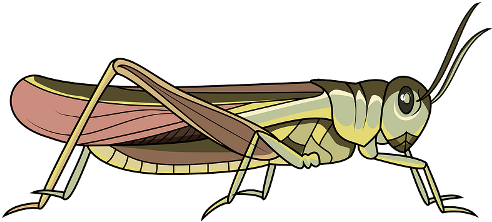
\includegraphics{locusta}
    \caption{locusta, -ae (f)}
\end{figure}%
ego indūcam crās locustam in\linebreak fīnēs tuōs:  quæ operiat
\mpp{superficiēs, -eī (f)}{pars superior vel summa alicuius reī}superficiem terræ, nē quidquam eius appāreat, sed
\mpp{comedere:}{totum ēsse; ēsse}comedātur quod \mpp{residuus/a/um:}{quod reliquum est}residuum
fuerit \mpp{grandō, grandinis (f):}{aqua frigidissima lapidī similis quae cadit dē
caelō}grandinī: \mpp{corrōdere:}{consumere}corrōdet enim omnia ligna quæ
\mpp{germinare:}{emittere germina (ea quae ex herbis veniunt semen,
fructus, cet.)}germinant in agrīs.  Et implēbunt domōs tuās, et servōrum
tuōrum, et omnium Ægyptiōrum, quantam nōn vīdērunt patrēs tuī, et \mpp{avus, -ī (m):}{pater patris vel matris}avī, ex
quō ortī sunt super terram, usque in præsentem diem. 

Āvertitque sē, et
ēgressus est ā Pharaōne.  Dīxērunt autem servī
Pharaōnis ad eum: \mpp{usquequō:}{usque ad quod tempus?}``Usquequō patiēmur hoc
\mpp{scandalum, -ī (n):}{rēs perdita}scandalum? Dīmitte hominēs, ut sacrificent Dominō Deō suō;
nōnne vidēs quod perierit Ægyptus?''

Revocāvēruntque Moysen et Aarōn ad
Pharaōnem, quī dīxit eīs: ``Īte, sacrificātē Dominō Deō vestrō: quīnam
sunt quī itūrī sunt?''

Ait Moysēs: ``Cum parvulīs nostrīs, et seniōribus
pergēmus, cum fīliīs et fīliābus, cum ovibus et \mpp{armentum, -ī (n):}{maiorum bestiarum grex (e.g: equōrum, bovum)}armentīs:
est enim \mpp{sōlemnitās, -ātis (f):}{diēs quī certīs temporibus quotannis fit quō homines deum servunt}sōlemnitās Dominī Deī nostrī.''

Et respondit
Pharaō: ``Sīc Dominus sit vōbīscum, quōmodo ego dīmittam
vōs, et parvulōs vestrōs, cui dubium est quod pessimē cōgitētis?  Nōn
fīet ita, sed īte tantum virī, et sacrificātē Dominō: hoc enim et ipsī
petīstis.''

Statimque ēiectī sunt dē cōnspectū Pharaōnis.  Dīxit autem
Dominus ad Moysēn: ``Extende manum tuam super terram Ægyptī ad locustam, ut
ascendat super eam, et dēvoret omnem herbam quæ \mpp{residuus/a/um:}{quod reliquum est}residua
fuerit \mpp{grandō, grandinis (f):}{aqua frigidissima lapidī similis quae cadit dē caelō}grandinī.''

Et extendit Moysēs virgam super terram Ægyptī: et
Dominus indūxit ventum ūrentem tōtā diē illā et nocte: et manē factō,
ventus ūrēns levāvit locustās.  Quæ ascendērunt super
ūniversam terram Ægyptī: et sēdērunt in cūnctīs fīnibus Ægyptiōrum
\mpp{innumerābilis, -e (adj):}{quī numerārī nōn potest}innumerābilēs, quālēs ante illud tempus nōn fuerant, nec
posteā futūræ sunt.  Operuēruntque ūniversam superficiem terræ,
\mpp{vastāre:}{percutere}vastantēs omnia. Dēvorāta est igitur herba terræ, et
quidquid \mimg{poma}{pōma\\pōmum, -ī (n)}pōmōrum in arboribus fuit, quæ grandō dīmīserat:
nihilque \mpp{omnino:}{vere, certe}omnīnō virēns relictum est in lignīs et
in herbīs terræ, in cūnctā Ægyptō.

Quam ob rem \mpp{festīnus/a/um:}{celeriter aliquid agens}festīnus
Pharaō vocāvit Moysen et Aarōn, et dīxit eīs: ``\mpp{peccatum:}{res contra
legem acta}Peccāvī in Dominum Deum vestrum, et in vōs.  Sed nunc
dīmittite peccātum mihi etiam hāc vice, et rogātē Dominum Deum vestrum, ut
auferat ā mē mortem istam.''

Ēgressusque Moysēs dē cōnspectū Pharaōnis,
ōrāvit Dominum.  Quī flāre fēcit ventum ab occidente
\mpp{vehemēns, -entis (adj):}{ferox, iratus, severus}vehementissimum, et \mpp{arripere:}{vī prehendere}arreptam locustam
prōiēcit in mare Rubrum: nōn remānsit nē ūna quidem in cūnctīs fīnibus
Ægyptī.  Et indūrāvit Dominus cor Pharaōnis, nec dīmīsit fīliōs
Isrāēl.  

Dīxit autem Dominus ad Moysēn: ``Extende manum
tuam in cælum: et sint tenebræ super terram Ægyptī tam
\mpp{densus/a/um:}{cuius partēs inter sē premunt}dēnsæ, ut \mpp{palpārī:}{leviter tangere}palpārī \mpp{queant =}{possint}queant.''

Extenditque
Moysēs manum in cælum: et factæ sunt tenebræ \mpp{horribilis, -e (adj):}{timendus/a/um}horribilēs in
ūniversā terrā Ægyptī tribus diēbus.  Nēmō vīdit frātrem suum, nec mōvit
sē dē locō in quō erat: \mpp{ubicumque:}{in omne locō in quō...}ubicumque autem habitābant fīliī
Isrāēl, lūx erat.

Vocāvitque Pharaō Moysen et Aarōn, et dīxit eīs: ``Īte,
sacrificātē Dominō: ovēs tantum vestræ et \mpp{armentum, -ī (n):}{maiorum bestiarum grex (e.g: equōrum, bovum)}armenta
remaneant, parvulī vestrī eant vōbīscum.''

Ait Moysēs: ``Hostiās quoque et
\mpp{holocaustum:}{sacrificium igne factum}holocausta dabis nōbīs, quæ offerāmus Dominō Deō nostrō. 
Cūnctī gregēs pergent nōbīscum; nōn remanēbit ex eīs
\mimg{hoof}{ungula, -ae (f)}ungula: quæ necessāria sunt in \mpp{cultus, -ūs (m):}{cura Deī}cultum Dominī Deī nostrī:
\mpp{praesertim:}{praecipue}præsertim cum ignōrēmus quid dēbeat
\mpp{immolāre:}{sacrificium facere}immolārī, dōnec ad ipsum locum
perveniāmus.''

Indūrāvit autem Dominus cor Pharaōnis, et nōluit dīmittere
eōs.  Dīxitque Pharaō ad Moysēn: ``Recēde ā mē, et cave nē ultrā videās
faciem meam: quōcumque diē appārueris mihi, moriēris.''

Respondit Moysēs: ``Ita fīet ut locūtus es: nōn vidēbō ultrā faciem tuam.''

\chapter{}

\titleimg{firstborn_title}

\mktitle{Capitulum Undecimum}
\thispagestyle{empty}

\cstart{E}{t} dīxit Dominus ad Moysēn: ``Adhūc ūnā
\mpp{plaga, ae (f):}{e.g, unus pulsat alterum; eo tempore cum pugnus corpus tangit
`plaga' vocatur}plāgā tangam Pharaōnem et Ægyptum, et post
hæc dīmittet vōs, et exīre \mpp{compellere:}{vī facere ut aliquis aliquid agat}compellet. \vnum{2}Dīcēs ergō omnī
\mpp{plēbs, plēbis (f):}{populus; praecipue hominēs quī pecuniosī non sunt ac minimam potestatem habent}plēbī ut postulet vir ab amīcō suō, et mulier ā
\mpp{vīcīnus/a/um:}{quī vel quae prope habitat}vīcīnā suā, vāsa argentea et aurea. \vnum{3}Dabit autem Dominus
grātiam populō suō cōram Ægyptiīs.''

Fuitque Moysēs vir
magnus valdē in terrā Ægyptī cōram servīs Pharaōnis et omnī
populō. \vnum{4}Et ait: ``Hæc dīcit Dominus: Mediā nocte ēgrediar in Ægyptum: 
\vnum{5}et moriētur omne \mpp{prīmōgenitus/a/um:}{quī vel quae prīmus natus est}prīmōgenitum in terrā Ægyptiōrum, ā
prīmōgenitō Pharaōnis, quī sedet in soliō eius, usque ad
prīmōgenitum ancillæ quæ est ad \mpp{mola, -ae (f):}{instrumentum grave quō frumentum premitur in minimās partēs}molam, et omnia
prīmōgenita \mpp{iumentum, -ī (n):}{animal utile ad gerendum vel
trahendum e.g, equi, boves, et cetera}iūmentōrum. \vnum{6}Eritque clāmor magnus
in ūniversā terrā Ægyptī, quālis nec ante fuit, nec posteā futūrus est. 
\vnum{7}Apud omnēs autem fīliōs Isrāēl nōn \mpp{mūtīre:}{parvā voce sonum facere vel loquī}mūtiet
canis ab homine usque ad pecūs: ut sciātis quantō \mpp{mīrāculum, -ī
(n):}{opus optime factum quod admirationem afferre potest}mīrāculō
dīvidat Dominus Ægyptiōs et Isrāēl. \vnum{8}Dēscendentque omnēs servī tuī istī ad
mē, et adōrābunt mē, dīcentēs: Ēgredere tū, et omnis populus quī
\mpp{subicere:}{facere ut aliquis alicui pareat}subiectus est tibi: post
hæc ēgrediēmur.''

\vnum{9}Et exīvit ā Pharaōne īrātus nimis. Dīxit
autem Dominus ad Moysēn: ``Nōn audiet vōs Pharaō ut multa
signa fīant in terrā Ægyptī.''

\vnum{10}Moysēs autem et Aarōn fēcērunt omnia
ostenta, quæ scrīpta sunt, cōram Pharaōne. Et \mpp{indurare:}{durum
facere}indūrāvit Dominus cor Pharaōnis, nec dīmīsit fīliōs Isrāēl dē terrā
suā. 

\chapter{}

\titleimg{birdhead}

\mktitle{Capitulum Duodecimum}
\thispagestyle{empty}

\vnum{1}Dīxit quoque Dominus ad Moysēn et Aarōn in terrā
Ægyptī: \vnum{2}``Mēnsis iste, vōbīs prīncipium mēnsium: prīmus erit in mēnsibus
annī. \vnum{3}Loquiminī ad ūniversum \mpp{cœtus, -ūs (m):}{grex hominum}\mimg{babygoat}{haedus, -ī (m)}cœtum fīliōrum Isrāēl, et
dīcite eīs: Decima diē mēnsis huius tollat ūnusquisque agnum per familiās
et domōs suās. \vnum{4}Sīn autem minor est numerus ut \mpp{sufficere:}{satis esse}sufficere
possit ad \mpp{vēscī:}{ēsse}vēscendum agnum, assūmet \mpp{vicinus/a/um:}{prope habitans}vīcīnum suum quī iūnctus est domuī suæ, iuxtā numerum
animārum quæ sufficere possunt ad ēsum agnī.''

\vnum{5}``Erit autem agnus absque
\mpp{macula, -ae (f):}{pars in quā proprius color abest}maculā,
\mpp{masculus/a/um:}{masculīnus}masculus, \mpp{anniculus/a/um:}{unius annī}anniculus:
iuxtā quem \mpp{rītus, -ūs (m):}{res agendae ut sacra recte fiant}rītum
tollētis et hædum. \vnum{6}Et
servābitis eum usque ad quartamdecimam diem mēnsis huius:
\mpp{immolare:}{sacrificium facere}immolābitque eum ūniversa multitūdō
fīliōrum Isrāēl ad \mpp{vespera, -ae (f) =}{vesper}vesperam.''

\begin{figure}[h!]
    \begin{minipage}[hp]{0.5\linewidth}
        \centering
        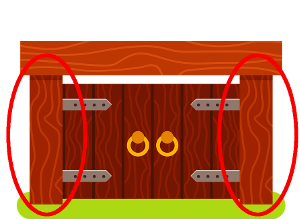
\includegraphics{postis}
        \caption{postis, -is (m)}
    \end{minipage}%
    \begin{minipage}[hp]{0.5\linewidth}
        \centering
        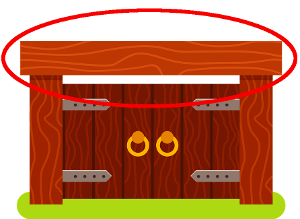
\includegraphics{superlimen}
        \caption{superlīmināre, -is (n)}
    \end{minipage}
\end{figure}

\vnum{7}``Et sūment dē sanguine eius,
ac pōnent super utrumque postem, et in
superlīmināribus \mimg{lactuca}{lactūca, -ae (f)}domōrum, in quibus \mpp{comedere:}{totum
esse; esse}comedent illum. \vnum{8}Et edent carnēs nocte illā
\mpp{assus/a/um}{sine aquā vel aliā materiā fluentī coctus}assās ignī, et
\mpp{azȳmus/a/um:}{sine materiā quae efficit ut panis turgidus fiat}azȳmōs pānēs cum lactūcīs \mpp{agrestis, -e (adj) <}{ager}agrestibus. \vnum{9}Nōn
comedētis ex eō \mpp{crūdus/a/um:}{non coctus}crūdum quid, nec coctum aquā, sed tantum
assum ignī: caput cum pedibus eius et intestīnīs
vorābitis.''

\begin{figure}[h!]
    \begin{minipage}[hp]{0.5\linewidth}
        \centering
        
\includegraphics{intestine}
        \caption{intestīnus, -ī (m)}
    \end{minipage}%
    \begin{minipage}[hp]{0.5\linewidth}
        \centering
        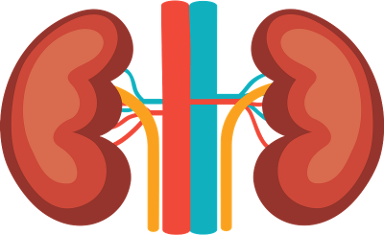
\includegraphics{renes}
        \caption{rēnēs, rēnum (m)}
    \end{minipage}
\end{figure}

\vnum{10}``Nec remanēbit quidquam ex eō usque manē; sī quid
\mpp{residuus:}{quod reliquum est}residuum fuerit, igne
\mpp{comburere:}{igne perdere}combūrētis. \vnum{11}Sīc autem comedētis illum:
\mpp{rēnēs accingere:}{induere vestis quae cingit corpus circiter rēnēs}rēnēs vestrōs \mpp{accingere =}{cingere}accingētis, et
\mpp{calceamentum:}{quod pedi induitur}calceāmenta habēbitis in pedibus,
tenentēs baculōs in manibus, et comedētis \mpp{festīnanter =}{celeriter}festīnanter: est
enim \mpp{Phase:}{vocabulum Hebraicum ``trānsitus'' significans}Phase (id est, trānsitus) Dominī. \vnum{12}Et trānsībō per
terram Ægyptī nocte illā, percutiamque omne \mpp{prīmōgenitus/a/um:}{quī vel quae prīmus natus est}prīmōgenitum in
terrā Ægyptī ab homine usque ad pecūs: et in cūnctīs dīīs Ægyptī faciam
\mpp{iūdicium, -ī (n):}{quod iudex tradit}\mimg{judge_small}{iudex, iudicis (m/f)}iūdicia. Ego Dominus. \vnum{13}Erit autem sanguis vōbīs in signum
in \mpp{aedēs, aedium (f pl.):}{aedificium}ædibus in quibus eritis: et vidēbō sanguinem, et
trānsībō vōs: nec erit in vōbīs \mpp{plāga, -ae (f):}{e.g, unus pulsat alterum eo
tempore cum pugnus corpus tangit `plāga' vocatur}plāgā
\mpp{disperdere:}{valde perdere}disperdēns quandō percusserō terram Ægyptī. \vnum{14}Habēbitis
autem hunc diem in \mpp{monumentum, -ī (n):}{quiquid nōs monet}monumentum: et
\mpp{celebrāre:}{agere quod oportet agere die Deō constitutō}celebrābitis eam \mpp{sōlemnis, -e (adj):}{sōlemnis dicitur de rēbus deō constitutibus quae certīs temporibus quotannis fit}sōlemnem Dominō in
\mpp{generātio, -ōnis (f):}{e.g: una generatio parentibus constat, līberīs eōrum altera generatio constat, etc...}generātiōnibus vestrīs cultū \mpp{sempiternus/a/um:}{perpetuus}sempiternō.
\vnum{15}Septem diēbus azȳma comedētis: in diē prīmō nōn erit
\mpp{fermentum, -ī (n):}{materia quae efficit ut panis turgidus fiat}fermentum in domibus vestrīs: quīcumque comēderit
\mpp{fermentō, -āre, -āvī, -ātum:}{ponere fermentum in aliquō}fermentātum, perībit anima illa dē Isrāēl, ā prīmō diē
usque ad diem septimum.''

\vnum{16}``Diēs prīma erit \mpp{sānctus/a/um:}{deō pertinens}sāncta atque
sōlemnis, et diēs septima eādem \mpp{fēstīvitās, -ātis (f):}{dies laetus deō constitutus}fēstīvitāte
\mpp{venerābilis, -e (adj):}{cultū dignus}venerābilis: nihil operis faciētis in eīs,
\mpp{exceptīs hīs:}{praeter hās}exceptīs hīs, quæ ad vēscendum \mpp{pertinere:}{e.g, colloquium ad me pertinet si homines loquuntur de me}pertinent. \vnum{17}Et
\mpp{observābitis azȳma:}{quotannis diem sanctam celebrētis in quā azymī panēs comeduntur}observābitis azȳma: in eādem enim ipsā diē ēdūcam
exercitum vestrum dē terrā Ægyptī, et cūstōdiētis diem istum in
generātiōnēs vestrās \mpp{rītus, -ūs (m):}{res agendae ut sacra recte fiant}rītū perpetuō.  \vnum{18} Prīmō mēnse, quartadecīmā diē mēnsis ad vesperam, comedētis
azȳma usque ad diem \mpp{vīgēsimam =}{vīcēsimam}vīgēsimam prīmam eiusdem mēnsis ad
vesperam. \vnum{19}Septem diēbus fermentum nōn inveniētur in domibus vestrīs:
quī comēderit fermentātum, perībit anima eius dē cœtū Isrāēl, tam dē
\mpp{advena, -ae (m)}{qui non est civis, qui ab alio loco venit}advenīs quam dē \mpp{indigena, -ae (adj)}{natus in eō lōcō}indigenīs terræ. \vnum{20}Omne fermentātum nōn
comedētis: in cūnctīs \mpp{habitāculum, -ī (n):}{locus in quō aliquis habitat}habitāculīs vestrīs edētis azȳma.''

\vnum{21}Vocāvit autem Moysēs omnēs seniōrēs fīliōrum Isrāēl, et
dīxit ad eōs: ``Īte tollentēs animal per familiās vestrās, et immolātē
Phase. \vnum{22}\mpp{fasciulum, -ī:}{multum lignī vel materiae aliae vinctum}Fasciculumque \mpp{hyssōpum, -ī (n):}{herba quaedam}hyssōpī
\mpp{tingere:}{humidum facere}tingite in sanguine quī est in līmine, et aspergite ex eō
superlīmināre, et utrumque postem: nūllus vestrum
ēgrediātur ōstium domūs suæ usque manē. \vnum{23}Trānsībit enim Dominus
percutiēns Ægyptiōs: cumque vīderit sanguinem in
superlīminārī, et in utrōque poste,
\mpp{trānscendere:}{transīre}trānscendet ōstium domūs, et nōn sinet
\mpp{percussōr, -ōris (m):}{quī percutit}percussōrem \mpp{ingredi:}{intus ire}ingredī domōs vestrās
et lædere. \vnum{24}Cūstōdī verbum istud \mpp{lēgitimus/a/um:}{qui secundum legēs est; iustus; verus}lēgitimum tibi et fīliīs
tuīs usque in \mpp{in aeternum:}{semper}æternum. \vnum{25}Cumque \mpp{introire:}{intus ire;
ingredi}introierītis terram, quam Dominus datūrus est vōbīs ut pollicitus
est, observābitis \mpp{cæremōnia, ae (f):}{res agendae ut sacra recte fiant}cæremōniās istās. \vnum{26}Et cum dīxerint
vōbīs fīliī vestrī: Quæ est ista \mpp{religiō, -ōnis (f):}{rītus}religiō? \vnum{27}Dīcētis eīs:
\mpp{victima, -ae (f):}{animal sacrificiō statutum}Victima trānsitūs Dominī est, quandō trānsīvit super
domōs fīliōrum Isrāēl in Ægyptō, percutiēns Ægyptiōs, et domōs nostrās
līberāns.''

\mimg{scimitar}{gladius \emph{incurvātus}}Incurvātusque populus adōrāvit. \vnum{28}Et ēgressī
fīliī Isrāēl fēcērunt sīcut \mpp{praecipere:}{imperare}præcēperat Dominus
Moȳsī et Aarōn. \vnum{29}Factum est autem in noctīs mediō, percussit Dominus omne
\mpp{prīmōgenitus/a/um:}{quī vel quae prīmus natus est}prīmōgenitum in terrā Ægyptī, ā prīmōgenitō
Pharaōnis, quī in soliō eius sedēbat, usque ad prīmōgenitum
\mpp{captīvus/a/um:}{qui captus, qui vinctus est}captīvæ quæ erat in carcere, et omne prīmōgenitum
\mpp{iumentum:}{animal utile ad gerendum vel trahendum e.g, equi, boves, et
cetera}iūmentōrum. \vnum{30}Surrēxitque Pharaō nocte, et omnēs
servī eius, cūnctaque Ægyptus: et ortus est clāmor magnus in Ægyptō:
neque enim erat domus in quā nōn iacēret mortuus. 

\vnum{31}Vocātīsque Pharaō
Moyse et Aarōn nocte, ait: ``Surgite et ēgrediminī ā populō
meō, vōs et fīliī Isrāēl: īte, immolātē Dominō sīcut dīcitis. \vnum{32}Ovēs
vestrās et \mpp{armentum, -ī (n):}{maiorum bestiarum grex (e.g: equōrum, bovum)}armenta assūmite ut petierātis, et abeuntēs
\mpp{benedīcere:}{sanctum facere}benedīcite mihi.''

\vnum{33}\mpp{urgēre:}{valde hortārī; cogere}Urgēbantque Ægyptiī
populum dē terrā exīre vēlōciter, dīcentēs: ``Omnēs moriēmur.''

\vnum{34}Tulit
igitur populus \mpp{cōnspergō, cōnspergere, cōnspersī, conspersum:}{spargere}cōnspersam \mpp{farīna, -ae (f):}{materia, aquā impositā, ex quā panis factus est}farīnam antequam
\mpp{fermentō, -āre, -āvī, -ātum:}{ponere fermentum in aliquō}fermentārētur: et ligāns in palliīs, posuit super
\mpp{humerōs =}{umerōs}humerōs suōs. \vnum{35}Fēcēruntque fīliī Isrāēl sīcut præcēperat
Moysēs: et petiērunt ab Ægyptiīs vāsa argentea et aurea, vestemque
plūrimam. \vnum{36}Dominus autem dedit grātiam populō cōram Ægyptiīs ut
\mpp{commodāre:}{libenter cum aliquō facere, libenter rēs dāre}commodārent eīs: et \mpp{spoliare:}{capere res aliorum
hominum}spoliāvērunt Ægyptiōs. 

\vnum{37}Profectīque sunt fīliī Isrāēl dē Ramesse
in Socoth, sexcenta ferē mīllia peditum virōrum, absque parvulīs. \vnum{38}Sed et
\mpp{vulgus, -ī (n):}{multitudo, turba}vulgus \mpp{prōmiscuus/a/um:}{mixtum}prōmiscuum \mpp{innumerabilis:}{qui
numerari non potest}innumerābile ascendit cum eīs, ovēs et armenta et
animantia \mpp{diversus:}{in varias partes versi sunt}dīversī generis multa
nimis. \vnum{39}Coxēruntque farīnam, quam \mpp{dūdum:}{nuper}dūdum dē Ægyptō
cōnspersam tulerant: et fēcērunt \mpp{subcinerīcus pānis:}{panis sub cinere coctus}subcinerīciōs pānēs
azȳmōs: neque enim poterant fermentārī, cōgentibus exīre
Ægyptiīs, et nūllam facere sinentibus moram: nec \mpp{pulmentum, -ī (n):}{cibus}pulmentī
quidquam occurrerat \mpp{praeparāre:}{parāre, ante parāre}præparāre.

\vnum{40}\mpp{habitātiō, -ōnis (f)}{actus habitandī}Habitātiō
autem fīliōrum Isrāēl quā mānsērunt in Ægyptō, fuit quadringentōrum
trīgintā annōrum. \vnum{41}Quibus \mpp{explere:}{perficere}explētīs, eādem diē
ēgressus est omnis exercitus Dominī dē terrā Ægyptī. \vnum{42}Nox ista est
\mpp{observāre:}{colere, servāre}\mpp{observābilis, -e (adj):}{quod potest observārī}observābilis Dominī, quandō ēdūxit eōs dē terrā Ægyptī: hanc
observāre dēbent omnēs fīliī Isrāēl in generātiōnibus suīs.

\vnum{43}Dīxitque Dominus ad Moysēn et Aarōn: ``Hæc est religiō Phase: omnis
\mpp{aliēnigena, -ae (m/f):}{aliō locō natus}aliēnigena nōn comedet ex eō. \vnum{44}Omnis autem servus
\mpp{emptitius =}{emptus}emptitius \mpp{circumcīdere:}{Removēre secandō summum membrum inter crura puerī vel virī situm}circumcīdētur, et sīc comedet. \vnum{45}Advena et
\mpp{mercēnārius, -ī (m):}{cui merces datur ut opus faciat}mercēnārius nōn edent ex eō. \vnum{46}In ūnā domō comedētur, nec
\mpp{efferre:}{extra ferre, proferre}efferētis dē carnibus eius forās, nec os illīus
\mpp{confringere:}{una frangere}cōnfringētis. \vnum{47}Omnis \mpp{cœtus, -ūs (m):}{grex hominum}cœtus fīliōrum
Isrāēl faciet illud. \vnum{48}Quod sī quis \mpp{peregrīnus/a/um:}{quī ex aliā terrā vēnit}peregrīnōrum in
vestram voluerit trānsīre \mpp{colōnia, -ae (f):}{locus in quō hominēs domūs novās confēcērunt et agrōs colere incēpērunt}colōniam, et facere Phase Dominī,
circumcīdētur prius omne masculīnum eius, et tunc \mpp{rītus, -ūs (m):}{res agendae ut sacra recte fiant}rīte
celebrābit: eritque sīcut \mpp{indigena, -ae (adj)}{natus in eō lōcō}indigena terræ:
sī quis autem circumcīsus nōn fuerit, nōn
\mpp{vēscī:}{ēsse}vēscētur ex eō. \vnum{49}Eādem lēx erit indigenæ
et colōnō quī \mpp{peregrinārī:}{iter facere per aliēna loca, patria procul abīre}peregrīnātur apud vōs.''

\vnum{50}Fēcēruntque omnēs
fīliī Isrāēl sīcut præcēperat Dominus Moȳsī et Aarōn. \vnum{51}Et eādem diē
ēdūxit Dominus fīliōs Isrāēl dē terrā Ægyptī per \mpp{turma, -ae (f):}{multitūdō}turmās
suās. 

\chapter{}

\titleimg{pillar}

\mktitle{Capitulum Tertium Decimum}
\thispagestyle{empty}

\cstart{L}{ocūtusque} est Dominus ad Moysen, dīcēns: \vnum{2}``\mpp{sānctificāre:}{sanctum facere}Sānctificā mihi omne \mpp{prīmōgenitus/a/um:}{quī vel quae prīmus natus est}prīmōgenitum quod
aperit vulvam \mpp{vulva, -ae (f):}{pars corporis feminae ubi infans crescit antequam paritur}\mpp{aperīre vulvam:}{parī}in fīliīs Isrāēl, tam dē
hominibus quam dē \mpp{iumentum:}{animal utile ad gerendum vel trahendum
e.g, equi, boves, et cetera}iūmentīs: mea sunt enim omnia.''

\vnum{3}Et ait
Moysēs ad populum: ``\mpp{mementōte =}{memoriā tenēte}Mementōte diēī huius in
quā ēgressī estis dē Ægyptō et dē domō servitūtis, quoniam in manū fortī
ēdūxit vōs Dominus dē locō istō: ut nōn \mpp{comedere:}{totum esse;
esse}comedātis \mpp{fermentō, -āre, -āvī, -ātum:}{ponere fermentum in aliquō}fermentātum pānem. \vnum{4}Hodiē ēgrediminī mēnsē
novārum frūgum. \vnum{5}Cumque \mpp{intrōdūcere:}{ducere intro}intrōdūxerit tē Dominus in terram
Chananæī, et Hethæī, et Amorrhæī, et Hevæī, et Iebusæī,
quam \mimg{iuro}{iurāre}iūrāvit patribus tuīs ut daret tibi, terram fluentem
lacte et melle, \mpp{celebrare:}{agere quod oportet agere die Deo
pertinenti}celebrābis hunc mōrem sacrōrum mēnse istō.
\vnum{6}Septem diēbus \mpp{vēscī:}{cibō utī}vēsceris \mpp{azȳma, -ae (f):}{sine fermentō}azȳmīs: et in diē septimō erit
\mpp{sōlemnitās, -ātis (f):}{dies qui certis temporibus quotannis fit quo homines deum
servunt}sōlemnitās Dominī. \vnum{7}Azȳma comedētis septem diēbus: nōn appārēbit
apud tē aliquid fermentātum, nec in cūnctīs fīnibus tuīs. \vnum{8}Nārrābisque
fīliō tuō in diē illō, dīcēns: Hoc est quod fēcit mihi Dominus quandō
ēgressus sum dē Ægyptō. \vnum{9}Et erit quasi signum in manū tuā, et quasi
\mpp{monimentum, -ī (n):}{quod nos monet}monimentum ante oculōs tuōs: et ut lēx Dominī semper sit
in ōre tuō, in manū enim fortī ēdūxit tē Dominus dē Ægyptō. \vnum{10}Cūstōdiēs
\mpp{huiuscemodī:}{huius modī}huiuscemodī cultum statūtō tempore ā diēbus in diēs. \vnum{11}Cumque intrōdūxerit
tē Dominus in terram Chananæī, sīcut iūrāvit tibi et patribus tuīs, et
dederit tibi eam: \vnum{12}\mpp{sēparāre:}{e.g, Habeō decem pilās in unō
locō, quinque rubrās et quinque atrās. Sumō rubrās et ponō eās in alterō
locō. Hōc modō sēparō rubrās ab atrīs.}Sēparābis omne quod aperit vulvam
Dominō, et quod \mpp{prīmitīvus/a/um:}{primo adveniens}prīmitīvum est in pecoribus tuīs: quidquid
habuerīs masculīnī \mpp{sexus, -ūs (m):}{id quō animal masculinum vel femininum esse dicitur}sexūs, 
\mpp{cōnsecrāre:}{sacrum facere}cōnsecrābis Dominō. \vnum{13}Prīmōgenitum asinī mūtābis ove: quod sī nōn redēmerīs,
interficiēs. Omne autem prīmōgenitum hominis dē fīliīs tuīs, pretiō
redimēs. \vnum{14}Cumque interrogāverit tē fīlius tuus crās, dīcēns: Quid est
hoc? respondēbis eī: In manū fortī ēdūxit nōs Dominus dē terrā Ægyptī, dē
domō servitūtis. \vnum{15}Nam cum \mpp{indurare:}{durum facere}indūrātus esset
Pharaō, et nōllet nōs dīmittere, occīdit Dominus omne
prīmōgenitum in terrā Ægyptī, ā prīmōgenitō hominis usque
ad prīmōgenitum iūmentōrum: \mpp{idcirco:}{propterea, ideo}idcircō
\mpp{immolare:}{sacrificium facere}immolō Dominō omne quod aperit vulvam
masculīnī sexūs, et omnia prīmōgenita fīliōrum meōrum
redimō. \vnum{16}Erit igitur quasi signum in manū tuā, et quasi
\mpp{appēndō, appendere, appendi, appensum:}{pendere}appēnsum quid, ob
\mpp{recordātiō, -ōnis (f) <}{recordārī: cogitāre dē aliquā memoriā}recordātiōnem, inter
oculōs tuōs: eō quod in manū fortī ēdūxit nōs Dominus dē Ægyptō. \vnum{17}Igitur
cum ēmīsisset Pharaō populum, nōn eōs dūxit Deus per viam terræ Philisthiim
quæ \mpp{vīcīnus/a/um:}{prope habitans}vīcīna est: \mpp{reputāre:}{cogitāre}reputāns nē forte
\mpp{pœnitet:}{e.g, si aliquem nocui et nunc me non nocuisse volo, me poenitet nocendī.}pœnitēret eum, sī vīdisset adversum sē bella
\mpp{consurgere:}{surgere}cōnsurgere, et reverterētur in Ægyptum. \vnum{18}Sed
\mpp{circum-dūcere}{}circumdūxit per viam dēsertī, quæ est iuxtā mare Rubrum:
et armātī ascendērunt fīliī Isrāēl dē terrā Ægyptī.''

\vnum{19}Tulit quoque Moysēs
ossa Ioseph sēcum: eō quod \mpp{adiūrāre:}{iūrāre}adiūrāsset fīliōs Isrāēl,
dīcēns: ``\mpp{visitare:}{visum ire}Vīsitābit vōs Deus;
\mpp{efferre:}{extra ferre, proferre}effertē ossa mea hinc vōbīscum.''

\vnum{20}Profectīque dē Socoth \mpp{castramētārī:}{castra ponere}castramētātī sunt in Etham, in
\mpp{extrēmus/a/um:}{ultimus, postremus}extrēmīs fīnibus \mpp{solitudo:}{deserta; locus ubi nemo
vel unus habitat}sōlitūdinis. \vnum{21}Dominus autem \mpp{praecēdere:}{ante īre}præcēdēbat
eōs ad ostendendam viam per diem in columnā nūbis, et per noctem in columnā
ignis: ut dux esset itineris utrōque tempore. \vnum{22}Numquam dēfuit columna
nūbis per diem, nec columna ignis per noctem, cōram populō. 

\chapter{}

\titleimg{drown}

\mktitle{Capitulum Quartum Decimum}
\thispagestyle{empty}

\cstart{L}{ocūtus} est autem Dominus ad Moysen, dīcēns: \vnum{2}``Loquēre
fīliīs Isrāēl: Reversī \mpp{castrametari:}{castra
ponere}castramētentur ē regiōne Phihahiroth, quæ est inter Magdalum et mare
contrā Beelsephon: in cōnspectū eius castra pōnētis super mare.
\vnum{3}Dictūrusque est Pharaō super fīliīs Isrāēl:
\mpp{coarctāre:}{in angustum cogere}Coarctātī sunt in terrā;
\mpp{conclūdere:}{claudere}conclūsit eōs
dēsertum. \vnum{4}Et \mpp{indurare:}{durum facere}indūrābō cor eius, ac
persequētur vōs: et \mpp{glōrificāre:}{gloriosum facere}glōrificābor in
Pharaōne, et in omnī exercitū eius; scientque Ægyptiī quia
ego sum Dominus. Fēcēruntque ita.''

\vnum{5}Et nūntiātum est rēgī Ægyptiōrum quod
fūgisset populus: \mpp{immūtātus/a/um:}{non mutatus}immūtātumque est cor
Pharaōnis et servōrum eius super populō, et dīxērunt: ``Quid
voluimus facere ut dīmitterēmus Isrāēl, nē servīret nōbīs?''

\vnum{6}Iūnxit ergō
currum, et omnem populum suum assūmpsit sēcum. \vnum{7}Tulitque sexcentōs currūs
ēlēctōs, et quidquid in Ægyptō curruum fuit: et ducēs tōtīus exercitūs.
\vnum{8}Indūrāvitque Dominus cor Pharaōnis rēgis Ægyptī, et persecūtus est fīliōs
Isrāēl: at illī ēgressī sunt in manū \mpp{excelsus/a/um:}{altus}excelsā.
\vnum{9}Cumque persequerentur Ægyptiī vestīgia \mpp{praecedere:}{ante
ire}præcēdentium, reperērunt eōs in castrīs super mare: omnis equitātus et
currūs Pharaōnis, et ūniversus exercitus, erant in Phihahiroth contrā
Beelsephon. 

\vnum{10}Cumque appropinquāsset Pharaō, levantēs fīliī Isrāēl oculōs,
vīdērunt Ægyptiōs post sē, et timuērunt valdē: clāmāvēruntque ad Dominum,
\vnum{11}et dīxērunt ad Moysēn: ``Forsitan nōn erant \mpp{sepulchrum, -ī (n):}{locus ubi mortuus positus est}sepulchra in
Ægyptō, ideō tulistī nōs ut morerēmur in \mpp{solitudo, -inis (f):}{deserta; locus ubi
nemo vel unus habitat}sōlitūdine: quid hoc facere voluistī, ut ēdūcerēs
nōs ex Ægyptō? \vnum{12}Nōnne iste est sermō, quem loquēbāmur ad tē in Ægyptō,
dīcentēs: Recēde ā nōbīs, ut serviāmus Ægyptiīs? Multō enim melius erat
servīre eīs, quam morī in sōlitūdine.''

\vnum{13}Et ait Moysēs ad
populum: ``Nōlīte timēre: stāte, et vidēte \mpp{magnālia, -ōrum (n.
pl.):}{res mirandae}magnālia Dominī
quæ factūrus est hodiē: Ægyptiōs enim, quōs nunc vidētis,
\mpp{nequaquam:}{minime, nullo modo}nēquāquam ultrā vidēbitis usque in
\mpp{sempiternus/a/um:}{perpetuus}sempiternum. \vnum{14}Dominus pugnābit prō vōbīs, et
vōs tacēbitis.''

\vnum{15}Dīxitque Dominus ad Moysēn: ``Quid clāmās ad mē? Loquere
fīliīs Isrāēl ut proficīscantur. \vnum{16}Tū autem \mpp{elevare:}{tollere; sursum
levare}ēlevā virgam tuam, et extende manum tuam super mare, et dīvide illud:
ut gradiantur fīliī Isrāēl in mediō marī per siccum. \vnum{17}Ego autem
indūrābō cor Ægyptiōrum ut persequantur vōs: et glōrificābor in Pharaōne,
et in omnī exercitū eius, et in curribus et in equitibus illīus. \vnum{18}Et
scient Ægyptiī quia ego sum Dominus cum glōrificātus fuerō
in Pharaōne, et in curribus atque in equitibus eius.''

\vnum{19}Tollēnsque sē
\mpp{angelus, -ī (m):}{res viva, sapiens, et potēns ā Deō missa quae agit quidquid Deus vult}angelus 
Deī, quī præcēdēbat castra Isrāēl, abiit post eōs:
et cum eō \mpp{pariter:}{aeque}pariter columna nūbis, priōra dīmittēns,
post tergum \vnum{20}stetit, inter castra Ægyptiōrum et castra Isrāēl: et erat
nūbēs \mpp{tenebrōsus/a/um:}{obscurus}tenebrōsa, et \mpp{illūmināre:}{illustrāre}illūmināns noctem, ita
ut ad sē \mpp{invicem:}{Aegyptiī, deinde filiī Isrāel}invicem tōtō noctis tempore accēdere nōn valērent.
\vnum{21}Cumque extendisset Moysēs manum super mare, abstulit illud Dominus
flante ventō \mpp{vehemens:}{ferox, iratus, severus}vehementī et \mpp{ūrere}{id quod ignis agit}ūrente
tōta nocte, et vertit in siccum: dīvīsaque est aqua. \vnum{22}Et
\mpp{ingredi:}{intus ire}ingressī sunt fīliī Isrāēl per medium siccī maris:
erat enim aqua quasi mūrus ā dextrā eōrum et læva. \vnum{23}Persequentēsque
Ægyptiī ingressī sunt post eōs, et omnis equitātus Pharaōnis, currūs eius
et equitēs per medium maris. \vnum{24}Iamque advēnerat vigilia
\mpp{mātūtīnus/a/um:}{quod in mane vel circum mane est}mātūtīna, et ecce \mpp{respicere:}{aspicere iuvandi
causa}respiciēns Dominus super castra Ægyptiōrum per columnam ignis et
nūbis, interfēcit exercitum eōrum, \vnum{25}et \mpp{sub-vertere:}{vertere aliquid ut summa pars ad fundum vertatur et fundus ad summam partem vertatur}subvertit
\mpp{profundus, -ī (m):}{fundus}\mimg{rota}{rota, -ae (f)}rotās curruum, ferēbanturque in profundum.

Dīxērunt ergō Ægyptiī: ``Fugiāmus Israēlem: Dominus enim
pugnat prō eīs contrā nōs.''

\vnum{26}Et ait Dominus ad Moysēn: ``Extende manum tuam
super mare, ut revertantur aquæ ad Ægyptiōs super currūs et equitēs
eōrum.''

\vnum{27}Cumque extendisset Moysēs manum contrā mare, reversum est prīmō
\mpp{diluculum, -ī (n):}{prima lux diei}dīlūculō ad priōrem locum: fugientibusque
Ægyptiīs occurrērunt aquæ, et \mpp{involvere:}{facere ut aliquid anguste circumdetur}involvit eōs Dominus in
mediīs flūctibus. \vnum{28}Reversæque sunt aquæ, et operuērunt currūs et equitēs
cūnctī exercitūs Pharaōnis, quī sequentēs ingressī fuerant mare: nec ūnus
quidem superfuit ex eīs. \vnum{29}Fīliī autem Isrāēl perrēxērunt per medium siccī
maris, et aquæ eīs erant quasi prō mūrō ā dextrīs et ā sinistrīs: 
\vnum{30}līberāvitque Dominus in diē illā Isrāēl dē manū Ægyptiōrum. 
\vnum{31}Et vīdērunt
Ægyptiōs mortuōs super \mpp{littus, -ōris (n):}{terra apud mare quae ā fluctibus pulsatur}littus maris, et manum magnam quam
exercuerat Dominus contrā eōs: timuitque populus Dominum, et crēdidērunt
Dominō et Moysī servō eius.

\invisiblechapter{Cap. XV}

\titleimg{mtitle}

\mktitle{Capitulum Quīntum Decimum}
\thispagestyle{empty}

\cstart{T}{unc} cecinit Moysēs et fīliī Isrāēl
carmen hoc Dominō, et dīxērunt:
\begin{flushleft}
{\it
    Cantēmus Dominō:\\
    glōriōsē enim magnificātus est,\\
    equum et \mpp{ascēnsor, -ōris (m):}{qui ascendit}ascēnsōrem \mpp{dēicere:}{deorsum iacere}dēiēcit in mare.

    \vnum{2}\mpp{fortitudo, -inis (f) <}{fortis}Fortitūdō mea, et laus mea Dominus,\\
    et factus est mihi in salūtem:\\
    iste Deus meus, et \mpp{glorificāre:}{gloriosum facere}glōrificābō eum:\\
    Deus patris meī, et \mpp{exaltāre:}{in altum levāre}exaltābō eum.

    \vnum{3}Dominus quasi vir pugnātor,\\
    \mpp{omnipotens, -entis (adj):}{habens omnem potestatem}Omnipotēns nōmen eius,

    \vnum{4}currus Pharaōnis et exercitum eius\\
    prōiēcit in mare:\\
    ēlēctī prīncipēs eius\\
    submersī sunt in marī Rubrō.

    \vnum{5}\mpp{abyssus, -ī (f):}{aqua cuius fundus longissime a nobis est}Abyssī operuērunt eōs;\\
    dēscendērunt in \mpp{profundum, -ī (n):}{fundus}profundum quasi \mimg{rock}{lapis, lapidis (m)}lapis.

    \vnum{6}Dextera tua, Domine,\\
    magnificāta est in fortitūdine:\\
    dextera tua, Domine,\\
    percussit inimīcum.

    \vnum{7}Et in multitūdine glōriæ tuæ\\
    dēposuistī \mpp{adversārius/a/um:}{qui est ante seu contra nos positus}adversāriōs tuōs:\\
    mīsistī īram tuam,\\
    quæ dēvorāvit eōs sīcut \mpp{stipula, -ae (f):}{media ac longa pars herbae ex quā aliae partēs extendunt}stipulam.

    \vnum{8}Et in \mpp{spiritus, -us (m):}{animus}spīritū \mpp{furōr, -ōris (m):}{qui habet `furorem' in sē valde perturbatur}furōris tuī\\
    \mpp{congregāre:}{in unum locum cogere vel ferre vel ducere}congregātæ sunt aquæ:\\
    stetit \mpp{unda, -ae (f):}{parvus fluctus}unda fluēns,\\
    congregātae sunt abyssī in mediō marī.

    \vnum{9}Dīxit inimīcus:\\
    Persequar et \mpp{comprehendere:}{prehendere}comprehendam,\\
    dīvidam \mpp{spolia, -ae (f):}{quod de hoste victo detrahitur}spolia,\\
    implēbitur anima mea:\\
    \mpp{ēvāgīnāre:}{ē vāgīnā educere}ēvāgīnābō gladium meum,\\
    interficiet eōs manus mea.

    \vnum{10}Flāvit spīritus tuus,\\
    et operuit eōs mare:\\
    submersī sunt quasi \mpp{plumbum, -ī (n):}{genus metallī}plumbum\\
    in aquīs \mpp{vehemens, -entis (adj):}{ferox, iratus, severus}vehementibus.

    \vnum{11}Quis similis tuī\\
    in fortibus, Domine?\\
    Quis similis tuī,\\
    magnificus in \mpp{sānctitās, -ātis (f) $<$}{sanctus}sānctitāte,\\
    terribilis atque \mpp{laudābilis, -is (adj):}{qui laudārī potest}laudābilis,\\
    faciēns mīrābilia? 
    
\vnum{12}Extendistī manum tuam,\\
et dēvorāvit eōs terra.
    
    \vnum{13}Dux fuistī in \mpp{misericordia, -ae (f):}{quod sentimus dum vidēmus aliquem patī}misericordiā tuā\\
    populō quem redēmistī:\\
    et portāstī eum in fortitūdine tuā,\\
    ad \mpp{habitaculum, -ī (n):}{locus in quo aliquis habitat}habitāculum sānctum tuum.

\vnum{14}Ascendērunt populī, et īrātī sunt:\\
dolōrēs \mpp{obtinēre:}{tenēre, habēre, possidēre}obtinuērunt \mpp{habitātor, -ōris (m):}{incola}habitātōrēs Philisthiim.

\vnum{15}Tunc conturbātī sunt prīncipēs Edom,\\
\mpp{robustus/a/um:}{durus, valens}rōbustōs Moab obtinuit tremor:\\
\mpp{obrigescō, obrigescere, obriguī:}{durus fierī}obriguērunt omnēs habitātōrēs Chanaan.

\vnum{16}\mpp{irruere:}{in aliquid vi se mittere}Irruat super eōs \mpp{formīdō, -ōnis (f):}{timor}formīdō et \mpp{pavor, -ōris (m):}{timor}pavor,\\
in \mpp{magnitudo, -udinis (f):}{quam magnum aliquid est}magnitūdine \mpp{brachium, -ī (n):}{bracchium}brāchiī tuī:\\
fīant \mpp{immōbilis, -e (adj):}{quī nōn movētur vel moverī non potest}immōbilēs quasi lapis,\\
dōnec \mpp{per-transīre:}{transīre per aliquid, praeter aliquid īre}pertranseat populus tuus, Domine,\\
dōnec pertranseat populus tuus iste,\\
quem possēdistī.

\vnum{17}\mpp{introducere:}{ducere intro}Intrōdūcēs eōs, et \mpp{plantāre:}{ponere herbam in terrā ut crescat}plantābis\\
in monte \mpp{haerēditās, -ātis (f):}{e.g, pater meus pecuniosus moritur et pecunia eius mihi datur - haec pecunia haerēditās vocātur}hærēditātis tuæ,\\
\mpp{firmus/a/um:}{durus; quod diu manet et nōn mutātur}firmissimō habitāculō tuō\\
quod operātus es, Domine:\\
\mpp{sānctuārium, -ī (n):}{sacer locus}sānctuārium tuum, Domine,\\
quod \mpp{firmāre:}{munīre; fortem facere}firmāvērunt manūs tuæ.

\vnum{18}Dominus rēgnābit\\
in \mpp{aeternus/a/um:}{quod neque principium neque finem temporis habet}æternum et ultrā.''
}
\end{flushleft}

\vnum{19}\mpp{ingredi:}{intus ire}\mimg{tymp}{tympanum, -ī (n)}Ingressus est enim eques Pharaō
cum curribus et equitibus eius in mare: et redūxit super eōs Dominus aquās
maris: fīliī autem Isrāēl ambulāvērunt per siccum in mediō eius. \vnum{20}
Sūmpsit ergō Maria \mpp{prophētissa, -ae (f):}{femina quae bene deum intellegit et de deō loquitur}prophētissa, 
soror Aarōn, tympanum in manū suā: 
egressæque sunt omnēs mulierēs post eam cum
tympanīs et \mpp{chorus, -ī (m):}{actus corporis movendi propter hominem cantantem vel similem}chorīs, \vnum{21}quibus
\mpp{praecinere:}{ante cantāre}præcinēbat, dīcēns: 

\begin{raggedright}
{\it

``Cantēmus Dominō,\\
glōriōsē enim magnificātus est:\\
equum et ascēnsōrem eius\\
dēiēcit in mare.''

}
\end{raggedright}


\invisiblechapter{Cap. XVI}

\titleimg{manna}

\mktitle{Capitulum Sextum Decimum}
\thispagestyle{empty}

\cstart{P}{rofectīque} sunt dē Elim, et vēnit omnis multitūdō fīliōrum
Isrāēl in dēsertum Sīn, quod est inter Elim et Sināī,
quintodecīmō diē mēnsis secundī, postquam ēgressī sunt dē terrā Ægyptī.

\vnum{2}Et \mpp{murmurāre:}{loqui de re quae non placet}murmurāvit omnis \mpp{congregātiō, -ōnis (f):}{grex hominum}congregātiō fīliōrum
Isrāēl contrā Moysēn et Aarōn in \mpp{sōlitūdo, -inis (f):}{locus ubi
nemo vel unus habitat}sōlitūdine. \vnum{3}Dīxēruntque fīliī Isrāēl ad eōs:
``Utinam mortuī essēmus per manum Dominī in terrā Ægyptī, quandō sedēbāmus
super \mimg{olla}{ōlla, -ae (f)}ōllās carnium, et \mpp{comedere:}{totum ēsse;
ēsse}comedēbāmus pānem in \mpp{saturitās, -ātis (f)}{< satis}saturitāte: cūr ēdūxistis nōs in
dēsertum istud, ut occīderētis omnem multitūdinem famē?''

\vnum{4}Dīxit autem
Dominus ad Moysēn: ``Ecce ego \mpp{pluere:}{imbrem facere}pluam vōbīs pānēs
dē cælō: ēgrediātur populus, et \mpp{colligere:}{invenīre rēs quae hīc illīc sunt, deinde sumere eās atque in unō locō ponere}colligat quæ
\mpp{sufficere:}{satis esse}sufficiunt per singulōs diēs: ut
\mpp{tentāre:}{conārī aliquid ut videatur quid fiat}tentem eum utrum ambulet in lēge meā, an nōn. \vnum{5}Dīē autem
sextō pārent quod \mpp{īnferre <}{in + ferre}īnferant: et sit \mpp{duplus/a/um:}{bis tantus}duplum
quam colligēre solēbant per singulōs diēs.''

\vnum{6}Dīxēruntque Moysēs et Aarōn ad omnēs fīliōs Isrāēl: ``Vespere sciētis
quod Dominus ēdūxerit vōs dē terrā Ægyptī, \vnum{7}et manē vidēbitis glōriam
Dominī: audīvit enim \mpp{murmur, murmuris (n):}{sonus hominis qui loquitur de re quae non placet}murmur vestrum contrā Dominum: nōs
vērō quid sumus, quia \mpp{mussitāre:}{parvā voce dicere}mussitāstis contrā nōs?''

\vnum{8}Et ait Moysēs: ``Dabit vōbīs Dominus vespere carnēs edere, et manē pānēs in
saturitāte: eō quod audierit \mpp{murmurātio, -ōnis (f) <}{murmurāre}murmurātiōnēs
vestrās quibus murmurātī estis contrā eum: nōs enim
quid sumus? Nec contrā nōs est murmur vestrum, sed contrā Dominum.''

\vnum{9}Dīxit quoque Moysēs ad Aarōn: ``Dīc ūniversæ \mpp{congregātiō, -ōnis (f):}{grex hominum}congregātiōnī
fīliōrum Isrāēl: Accēdite cōram Dominō: audīvit enim murmur vestrum.''

\vnum{10}Cumque loquerētur Aarōn ad omnem \mpp{cœtus, -ūs (m):}{congregātiō}cœtum fīliōrum Isrāēl, \mpp{respicere:}{aspicere iuvandī
causā}respexērunt ad sōlitūdinem: et ecce glōria Dominī appāruit in nūbe.

\vnum{11}Locūtus est autem Dominus ad Moysen, dīcēns: \vnum{12}``Audīvī murmurātiōnēs
fīliōrum Isrāēl. Loquere ad eōs: Vespere comedētis carnēs, et manē
\mpp{saturāre:}{tam multum ēsse ut fortasse dicas ``bene, bene, satis est!''}saturābiminī pānibus: sciētisque quod ego sum Dominus Deus
vester.''

\begin{figure}[h!]
    \begin{minipage}[hp]{0.5\linewidth}
        \centering
        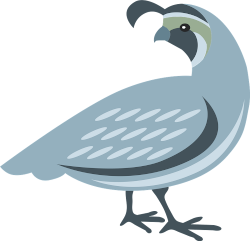
\includegraphics{quail}
        \caption{coturnīx, -īcis (f)}
    \end{minipage}%
    \begin{minipage}[hp]{0.5\linewidth}
        \centering
        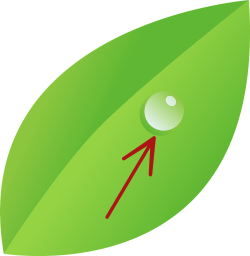
\includegraphics{dew}
        \caption{rōs, rōris (m)}
    \end{minipage}
\end{figure}

\vnum{13}Factum est ergō vespere, et ascendēns coturnīx
\mpp{cooperīre:}{operīre}cooperuit \mpp{coturnīx cooperuit castra:}{coturnīcēs cooperuērunt castra}castra: manē 
quoque rōs iacuit per \mpp{circuitus, -ūs (m):}{locus circum alterum
locum}circuitum castrōrum. \vnum{14}Cumque operuisset \mpp{superficiēs, -eī (f):}{summa pars reī quae operit aliās īnferiorēs partēs}superficiem
terræ, appāruit in
sōlitūdine \mpp{minūtus/a/um:}{parvus}minūtum, et quasi \mpp{pilum, -ī (n):}{baculum minimum quō homo herbās aliāsque rēs frangit in parvō poculō} pilō \mpp{tūsus/a/um:}{pulsatus}tūsum in
\mpp{in similitūdinem pruīnae:}{similis pruīnae}similitūdinem \mpp{pruīna, -ae (f):}{rōs frigidissimus}pruīnæ super terram. \vnum{15}Quod
cum vīdissent fīliī Isrāēl, dīxērunt ad \mpp{ad invicem:}{inter sē}invicem: ``Manhu?'' quod significat: ``Quid est
hoc?'' Ignōrābant enim quid esset. 

Quibus ait Moysēs: ``Iste est pānis quem
Dominus dēdit vōbīs ad \mpp{vēscī:}{ēsse}vēscendum. \vnum{16}Hic est sermō, quem
\mpp{praecipere:}{imperāre}præcēpit Dominus: Colligat ūnusquisque ex eō
quantum sufficit ad vēscendum: \mpp{gomor:}{mensura Hebraeōrum}gomor per singula capita,
iuxtā numerum animārum vestrārum quæ habitant in
\mimg{tab2}{tabernāculum, -ī (n)}tabernāculō sīc tollētis.''

\vnum{17}Fēcēruntque ita fīliī Isrāēl:
et collēgērunt, alius plūs, alius minus. \vnum{18}\mpp{mētior, mētīrī, mēnsus sum:}{e.g, homo habet magnum vas aquae plenum et oportet eum fundere aquam in decem alia parva vasa. Dicimus hominem mētīrī aquam}Et mēnsī sunt
ad \mpp{mēnsūra, -ae (f):}{e.g, ``da mihi decem vasa aquae plena!'' Vas dicitur mēnsūra aquae}
mēnsūram gomor: nec quī plūs collēgerat, habuit
\mpp{amplius =}{plus}amplius: nec quī minus parāverat, reperit minus: sed
singulī iuxtā id quod edere poterant, \mpp{congregāre:}{in unum locum
cōgere vel ferre vel ducere}congregāvērunt. 

\vnum{19}Dīxitque Moysēs ad eōs: ``Nūllus relinquat ex eō in manē.''

\vnum{20}Quī nōn audiērunt eum, sed
dīmīsērunt quīdam ex eīs usque manē, et \mimg{vermis}{vermis, -is (m)}\mpp{scatēre:}{plēnum esse}scatēre cœpit
vermibus, atque \mpp{computrēscere:}{facere malum odorem
(id quod nasus sentit) propter rem mortuam}computruit: et īrātus est
contrā eōs Moysēs. \vnum{21}Colligēbant autem māne singulī,
quantum sufficere poterat ad vēscendum: cumque \mpp{incalesco, incalescere, incaluī:}{valde calidus fiērī}incaluisset
sōl, \mpp{liquefiērī:}{fiērī res fluens sicut aqua}liquefiēbat. \vnum{22}In diē autem sextā collēgērunt cibōs
\mpp{duplex, duplicis (adj):}{bis tantus}duplicēs, id est, duo gomor per singulōs hominēs: vēnērunt
autem omnēs prīncipēs multitūdinis, et nārrāvērunt Moȳsī. 

\vnum{23}Quī ait eīs:
``Hoc est quod locūtus est Dominus: \mpp{requiēs, requiēī (f):}{tempus quo homo non
laborat}Requiēs \mpp{sabbatum, -ī (n):}{dies septimus quō non licet hominibus laborāre}sabbatī \mpp{sānctificāre:}{sanctum
facere}sānctificāta est Dominō crās: quodcumque operandum est, facite, et
quæ coquenda sunt coquite: quidquid autem reliquum fuerit, repōnite usque
in manē.''

\vnum{24}Fēcēruntque ita ut præcēperat Moysēs, et nōn computruit, neque
vermis inventus est in eō.

\vnum{25}Dīxitque Moysēs: ``Comedite
illud hodiē, quia sabbatum est Dominī: nōn inveniētur
hodiē in agrō. \vnum{26}Sex diēbus colligite: in diē autem
septimō sabbatum est Dominī, \mpp{idcircō:}{proptereā, ideō}idcircō nōn
inveniētur.''

\vnum{27}Venitque septima diēs: et ēgressī dē populō ut
colligerent, nōn invēnērunt.

\vnum{28}Dīxit autem Dominus ad
Moysēn: ``\mpp{usquequō:}{usque ad quod tempus?}Us\-quequō nōn vultis
cūstōdīre \mpp{mandātum, -ī (n):}{id quod imperatum vel traditum
est}mandāta mea et lēgem meam? \vnum{29}Vidēte quod Dominus dederit vōbīs
sabbatum, et propter hoc diē sextā \mpp{tribuere:}{dāre}tribuit vōbīs cibōs
duplicēs: maneat ūnusquisque apud \mpp{sēmetipsum =}{sē}sēmetipsum; nūllus
ēgrediātur dē locō suō diē septimō.''

\vnum{30}Et \mpp{sabbatīzāre:}{sabbatum colere}sabbatīzāvit
populus diē septimō. \linebreak\vnum{31}Appellāvitque domus Isrāēl nōmen eius\linebreak Mān: quod erat quasi sēmen
\mpp{coriandrum, -ī (n):}{quaedam herba}coriandrī album, \mpp{gustus, -ūs (m) < gustāre}{}gustusque eius quasi
similæ cum melle.

\vnum{32}Dīxit autem Moysēs: ``Iste est sermō, quem præcēpit
Dominus: Implē gomor ex eō, et cūstōdiātur in futūrās
retrō \mpp{generātio, -ōnis (f):}{e.g una generatio
parentibus constat, līberīs eōrum altera generatio constat,
etc...}generātiōnēs: ut nōverint pānem, quō aluī vōs in sōlitūdine, quandō
ēductī estis dē terrā Ægyptī.''

\vnum{33}Dīxitque Moysēs ad Aarōn: ``Sūme vās ūnum,
et mitte ibi mān, quantum potest capere gomor, et repōne cōram Dominō ad
servandum in generātiōnēs vestrās, \vnum{34}sīcut præcēpit Dominus Moȳsī.''

Posuitque illud Aarōn in tabernāculō reservandum. \vnum{35}Fīliī autem Isrāēl
comēdērunt mān quadrāgintā annīs, dōnec venīrent in terram \mpp{habitābilis, -e (adj):}{habitārī potest}habitābilem: hōc cibō alitī sunt, us\-quequō
tangerent fīnēs terræ Chanaan.

\vnum{36}Gomor autem decima pars
est \mpp{ephī (n) (indec):}{mensura Hebraeōrum}ephī.

\invisiblechapter{Cap. XVII}

\titleimg{arms.jpg}

\mktitle{Capitulum Septimum Decimum}
\thispagestyle{empty}


\cstart{I}{gitur} profecta omnis multitūdō fīliōrum Isrāēl dē
dēsertō Sīn per \mpp{mānsiō, -ōnis (f):}{locus ubi iter facientes noctu manent}mānsiōnēs suās, iuxtā sermōnem Dominī,
\mpp{castramētārī:}{castra ponere}castramētātī sunt in Raphidim, ubi nōn
erat aqua ad bibendum populō. 

\vnum{2}Quī \mpp{iurgārī:}{querī}iūrgātus contrā
Moysēn, ait: ``Dā nōbīs aquam, ut bibāmus.''

Quibus respondit Moysēs: ``Quid iūrgāminī contrā mē? Cūr
\mpp{tentāre:}{conārī aliquid ut videatur quid fiat}tentātis Dominum?''

\vnum{3}Sitīvit ergō ibi populus præ aquæ \mpp{pēnūria, -ae (f):}{id quod paene minus sit quam necesse est}pēnūriā, et
\mpp{murmurāre:}{loqui de re quae non placet}murmurāvit contrā Moysen,
dīcēns: Cūr fēcistī nōs exīre dē Ægyptō, ut occīderēs nōs, et līberōs
nostrōs, ac \mpp{iūmentum, -ī (n):}{animal utile ad gerendum vel trahendum e.g, equī, bovēs, et cetera}iūmenta sitī? 

\vnum{4}Clāmāvit autem Moysēs ad
Dominum, dīcēns: ``Quid faciam populō huic? Adhūc \mpp{paululum =}{paulum}paululum,
et \mimg{rock}{lapis, lapidis (m)}\mpp{lapidāre:}{lapidēs iacere}lapidābit mē.''

\vnum{5}Et ait Dominus ad Moysēn:
\mpp{antecēdere:}{ante īre}``Antecēde populum, et sūme tēcum dē seniōribus Isrāēl: et
virgam quā percussistī fluvium, tolle in manū tuā, et vāde. 
\vnum{6}Ēn ego stābō ibi cōram tē, suprā \mpp{petra, -ae (f):}{lapis}petram
Horeb: percutiēsque petram, et exībit ex eā aquā, ut bibat
populus.''

Fēcit Moysēs ita cōram seniōribus Isrāēl 
\vnum{7}et vocāvit nōmen locī
illīus, \mpp{tentātiō, -ōnis (f) <}{tentāre}Tentātiō, propter \mpp{iūrgium, -ī (n) <}{iūrgārī}iūrgium fīliōrum
Isrāēl, et quia tentāvērunt Dominum, dīcentēs: ``Estne Dominus in nōbīs, an
nōn?''

\vnum{8}Venit autem Amalec, et pugnābat contrā Isrāēl in Raphidim.
\vnum{9}Dīxitque Moysēs ad Iōsue: ``Ēlige virōs: et ēgressus, pugnā contrā Amalec:
crās ego stābō in \mpp{vertex, verticis (m):}{altissima pars}vertice collis, habēns virgam Deī in manū
meā.''

\vnum{10}Fēcit Iōsue ut locūtus erat Moysēs, et pugnāvit contrā Amalec:
Moysēs autem et Aarōn et Hur ascendērunt super verticem
collis. 
\vnum{11}Cumque levāret Moysēs manūs, vincēbat Isrāēl: sīn autem
paululum remīsisset, \mpp{superāre:}{vincere}superābat Amalec. 
\vnum{12}Manūs autem Moȳsī
erant gravēs: sūmentēs igitur \mimg{rock}{lapis, lapidis (m)}lapidem, posuērunt
\mpp{subter $\leftrightarrow$}{super}subter eum, in quō sēdit: Aarōn autem et Hur
\mpp{sustentāre:}{sustinēre}sustentābant manūs eius ex utrāque parte. Et factum est ut
manūs illīus nōn \mpp{lassāre:}{fatigāre}lassārentur usque ad occāsum sōlis. 
\vnum{13}Fugāvitque Iōsue Amalec, et populum eius in ōre gladiī. 

\vnum{14}Dīxit autem
Dominus ad Moysēn: ``Scrībe hoc ob \mpp{monimentum, -ī (n):}{quod nos
monet}monimentum in librō, et trāde auribus Iōsue: dēlēbō enim memoriam
Amalec sub cælō.'' 

\vnum{15}Ædificavitque Moysēs altāre: et vocāvit nōmen eius
`Dominus \mpp{exaltātiō, -ōnis (f) < }{exaltāre (in altum levāre)}exaltātiō mea' dīcēns: 
\vnum{16}``Quia manus soliī Dominī,
et bellum Dominī erit contrā Amalec, ā \mpp{generātio, -ōnis (f):}{e.g una
generatio parentibus constat, līberīs eōrum altera generatio constat,
etc...}generātiōne in generātiōnem.''

\chapter{}

\titleimg{arms.jpg}

\mktitle{Capitulum Duodevicesimum}
\thispagestyle{empty}

\cstart{C}{umque} audīsset Iethrō, \mpp{sacerdōs, -ōtis (m):}{quī res sacrās agit vel qui ducit aliōs in rēbus sacrīs agendīs}sacerdōs Mad\-ian, \mpp{cognātus/a/um (adj):}{qui pars eiusdem familiae est -- Iethrō est pater uxoris Moysī}cognātus Moȳsī,
omnia quæ fēcerat Deus Moȳsī, et Israēlī populō suō, et
quod ēdūxisset Dominus Isrāēl dē Ægyptō, 
\vnum{2}tulit Sephoram
uxōrem Moȳsī quam remīserat, 
\vnum{3}et duōs fīliōs eius: quōrum ūnus vocābātur
Gersam, dīcente patre: \mpp{advena, -ae (m/f):}{quī non civis est, quī in terrā aliā natus est}``Advena fuī in terrā aliēnā;'' 
\vnum{4}alter vērō Eliezer:
``Deus enim,'' ait, ``patris meī \mpp{adiūtor, -ōris (m):}{qui adiuvat}adiūtor
meus, et ēruit mē dē gladiō Pharaōnis.'' 

\vnum{5}Venit ergō Iethrō
cognātus Moȳsī, et fīliī eius, et uxor eius ad Moysēn in
dēsertum, ubi erat \mpp{castramētārī:}{castra ponere}castramētātus iuxtā
montem Deī. 
\vnum{6}Et \mpp{mandātum, -ī (n):}{id quod imperatum vel traditum
est}mandāvit Moysī, dīcēns: ``Ego Iethrō cognātus tuus veniō
ad tē, et uxor tua, et duo fīliī cum eā.'' 

\vnum{7}Quī ēgressus in occursum
cognātī suī, adōrāvit, et ōsculātus est eum:
salūtāvēruntque sē \mpp{mūtuō salūtāvērunt:}{Hic illum salūtāvit et ille hunc salūtāvit}mūtuō verbīs \mpp{pācificus/a/um:}{pacem faciens}pācificīs. Cumque intrāsset
\mimg{tab2}{tabernaculum, -ī (n)}tabernāculum, 
\vnum{8}nārrāvit Moysēs
cognātō suō cūncta quæ fēcerat Dominus
Pharaōnī et Ægyptiīs propter Isrāēl: ūniversumque labōrem,
quī accidisset eīs in itinere, et quod līberāverat eōs Dominus.
\vnum{9}Lætatusquē est Iethrō super omnibus bonīs, quæ fēcerat Dominus Israēlī, eō
quod ēruisset eum dē manū Ægyptiōrum. 

\vnum{10}Et ait: ``\mpp{benedīcere:}{sanctum facere}Benedictus Dominus, quī līberāvit vōs dē manū Ægyptiōrum, et dē manū
Pharaōnis; quī ēruit populum suum dē manū Ægyptī. 
\vnum{11}Nunc cognōvī, quia
magnus Dominus super omnēs deōs: eō quod superbē ēgerint contrā illōs.''

\vnum{12}Obtulit ergō Iethrō cognātus Moȳsī \mpp{holocaustum:}{sacrificium igne
factum}holocausta et hostiās Deō: vēnēruntque Aarōn et omnēs seniōrēs
Isrāēl, ut \mpp{comedere:}{totum ēsse; ēsse}comederent pānem cum eō cōram
Deō. 
\vnum{13}Alterā autem diē sēdit Moysēs ut \mpp{iudicāre:}{quod iudex
agit}iūdicāret populum, quī \mpp{assistere:}{stāre ad aliquid vel prope aliquid}assistēbat Moȳsī ā māne usque
ad \mpp{vespera, -ae (f):}{vesper}vesperam. 
\vnum{14}Quod cum vīdisset cognātus
eius omnia scīlicet quæ agēbat in populō, ait: ``Quid est hoc quod facis in
\mpp{plēbs, plēbis (f):}{populī multitudo}plēbe? Cūr sōlus sēdēs, et omnis populus
\mpp{præstōlārī:}{stāre ante aliquem et expectāre}præstōlātur dē māne usque ad vesperam?''

\vnum{15}Cui respondit
Moysēs: ``Venit ad mē populus quærēns sententiam Deī: 
\vnum{16}cumque acciderit
eīs aliqua \mpp{disceptātiō, -ōnis (f):}{e.g, unus dicit alterum malum facere, et alter se defendit -- hoc est disceptātiō}disceptātiō, veniunt ad mē ut
\mpp{iūdicium, -ī:}{quod iudex tradit}iūdicem inter eōs, et ostendam
\mpp{praeceptum, -ī:}{quod praecipitur}præcepta Deī, et lēgēs eius.''

\vnum{17}At ille: ``Nōn bonam, inquit, rem facis. 
\vnum{18}Stultō labōre cōnsūmeris et tū, et
populus iste quī tēcum est: ultrā vīrēs tuās est negōtium; sōlus illud
nōn poteris sustinēre. 
\vnum{19}Sed audī verba mea atque cōnsilia, et erit Deus
tēcum. Ēsto tū populō in hīs quæ ad Deum \mpp{pertinēre:}{e.g, colloquium
ad mē pertinet sī hominēs loquuntur dē mē}pertinent, ut referās quæ
dīcuntur ad eum: 
\vnum{20}ostendāsque populō \mpp{cæremōnia, ae (f):}{res agendae ut sacra recte fiant}cæremōniās et
\mpp{rītus, -ūs (m):}{cæremōnia}rītum colendī,
viamque per quam \mpp{ingredī:}{intus īre}ingredī dēbeant, et opus quod
facere dēbeant. 
\vnum{21}\mpp{prōvidēre:}{curāre ut aliquid habeās}Prōvidē autem dē omnī plēbe virōs
\mpp{potēns, potentis (adj):}{qui multas res agere potest: e.g, dux, rēx}potentēs, et timentēs Deum, in quibus sit vēritās, et quī
ōderint \mpp{avāritia, -ae (f):}{amor pecuniae}avāritiam, et cōnstitue ex eīs
\mpp{tribūnus, -ī (m):}{dux multōrum}tribūnōs, et \mpp{centuriō, -ōnis (m):}{dux centum hominum}centuriōnēs, et
\mpp{quīnquāgēnāriō, -ōnis (m):}{dux quīnquāgīnta hominum}quīnquāgēnāriōs, et \mpp{decānus, -ī (m):}{dux decem hominum}decānōs, 
\vnum{22}quī
iūdicent populum omnī tempore: quidquid autem maius fuerit, referant ad
tē, et ipsī minōra \mpp{tantummodo =}{solum}tantummodo iūdicent: leviusque sit
tibi, partītō in aliōs \mpp{onus, oneris (n):}{res quam difficile est
portare vel agere. e.g saccus lapidibus plenus, labor difficilis}onere.
\vnum{23}Sī hoc fēcerīs, implēbis imperium Deī, et præceptā eius poteris
\mpp{sustentāre:}{sustinēre}sustentāre: et omnis hīc populus revertētur ad
loca sua cum pāce.'' 

\vnum{24}Quibus audītis, Moysēs fēcit omnia quæ ille
\mpp{suggerere:}{offerre consilium}suggesserat. 
\vnum{25}Et ēlēctīs virīs \mpp{strēnuus/a/um:}{impiger, industrius}strēnuīs
dē cūnctō Isrāēl, cōnstituit eōs prīncipēs populī, tribūnōs, et
centuriōnēs, et quīnquāgēnāriōs, et decānōs. 
\vnum{26}Quī iūdicābant
\mpp{plēbs, plēbis}{populī multitudo}plēbem omnī tempore: quidquid autem gravius erat,
referēbant ad eum, faciliōra tantummodo iūdicantēs. 
\vnum{27}Dīmīsitque
cognātum suum: quī reversus abiit in terram suam. 

\chapter{}

\titleimg{tencommand}

\mktitle{Capitulum Undevicesimum}
\thispagestyle{empty}

\cstart{M}{ēnse} tertiō \mpp{ēgressiō, -ōnis (f) <}{ēgredī}ēgressiōnis Isrāēl dē
terrā Ægyptī, in diē hāc vēnērunt in \mpp{sōlitūdo, -inis ($<$
solus/a/um):}{deserta; locus ubi nemo vel unus habitat}sōlitūdinem Sināī. 
\vnum{2}Nam profectī dē Raphidim, et pervenientēs usque in dēsertum Sināī,
\mpp{castramētārī:}{castra ponere}castramētātī sunt in eōdem locō, ibique
Isrāēl fīxit \mimg{tab2}{tentōrium, -ī (n)}tentōria ē regiōne montis. 

\vnum{3}Moysēs autem ascendit ad Deum: vocāvitque eum Dominus dē
monte, et ait: ``Hæc dīcēs domuī Iācōb, et
\mpp{annūntiāre:}{nuntiāre}annūntiābis fīliīs Isrāēl: 
\vnum{4}Vōs ipsī vīdistis quæ fēcerim
Ægyptiīs, quōmodo portāverim vōs super ālās aquilārum, et \mpp{assūmere:}{sumere ad sē; iungere sibi}assūmpserim mihi.
\vnum{5}Sī ergō audierītis vōcem meam, et cūstōdieritis \mpp{pactum, -ī
(n):}{quod inter aliquōs convenit}pactum meum, eritis mihi in pecūlium dē
cūnctīs populīs: mea est enim omnis terra: 
\vnum{6}et vōs eritis mihi in
\mpp{rēgum, rēgī (n):}{quod rēx rēgit}rēgnum \mpp{sacerdōtālis, -e (adj) <}{sacerdōs}sacerdōtāle, et gēns
sāncta. Hæc sunt verba quæ loqueris ad fīliōs
Isrāēl.''

\vnum{7}Venit Moysēs: Et convocātīs maiōribus nātū populī, exposuit
omnēs sermōnēs quōs \mpp{mandātum, -ī (n):}{id quod imperatum vel traditum
est}mandāverat Dominus. 

\vnum{8}Responditque omnis populus simul: ``Cūn\-cta quæ
locūtus est Dominus, faciēmus.''

Cumque retulisset Moysēs verba populī ad
Dominum, \vnum{9}ait eī Dominus: ``Iam nunc veniam ad tē in
\mpp{cālīgō, cālīginis (f):}{aer per quem difficile est vidēre}cālīgine nūbis, ut audiat mē populus loquentem ad tē, et
crēdat tibi in perpetuum.''\mimg{bucina}{buccina, -ae (f)}


Nūntiāvit ergō Moysēs verba populī ad Dominum.  \vnum{10}Quī dīxit eī: ``Vāde ad populum, et \mpp{sānctificāre:}{sanctum
facere}sānctificā illōs hodiē, et crās, laventque vestīmenta sua. 
\vnum{11}Et sint parātī in diem tertium: in diē enim tertiā dēscendet Dominus cōram
omnī \mpp{plēbs, plēbis (f):}{populus; praecipue hominēs quī pecuniosī non sunt ac minimam potestatem habent}plēbe super montem Sināī. 
\vnum{12}Cōnstituēs\-que \mpp{terminus, -ī (m):}{finis terrae}terminōs populō per \mpp{circuitus, -ūs
(m):}{locus circum alterum locum}\mimg{rock}{lapis, lapidis (m)}circuitum, et dīcēs ad eōs: Cavēte nē
ascendātis in montem, nec tangātis fīnēs illīus: omnis quī tetigerit
montem, morte moriētur.
\vnum{13}Manus nōn tanget eum, sed
lapidibus \mpp{opprimere:}{premere aliquem ne surgere possit}opprimētur, aut \mpp{cōnfodere:}{vulnerāre}cōnfodiētur \mpp{iaculum, -ī (n):}{quiquid iacī potest ut aliquis vulnerētur}iaculīs:
sīve \mpp{iūmentum, -ī (n):}{animal utile ad gerendum vel trahendum e.g,
equī, bovēs, et cetera}iūmentum fuerit, sīve homō, nōn vīvet: cum cœperit
\mpp{clangere:}{facere sonum magnum ut tuba}clangere buccina, tunc ascendant in montem.''

\vnum{14}Dēscenditque Moysēs dē monte ad populum, et sānctificāvit eum. Cumque
lāvissent vestīmenta sua, 
\vnum{15}ait ad eōs: ``Ēstote parātī in diem tertium, et
nē appropinquētis uxōribus vestrīs.''

\vnum{16}Iamque advēnerat tertius diēs, et
manē inclāruerat: et ecce cœpērunt audīrī \mpp{tonitruum, -ī (n):}{tonitrus}tonitrua, ac
\mpp{micāre:}{lucem mittere ut ignis, stellae, et cetera}micāre fulgura, et nūbēs \mpp{densus/a/um:}{cuius partēs
inter sē premunt}dēnsissima operīre montem, \mpp{clangor, -ōris (m):}{strepitus}clangorque
buccinæ \mpp{vehemens, -entis (adj):}{ferox, iratus, severus}vehementius
\mpp{perstrepere:}{strepitum magnum facere}perstrepēbat: et timuit populus quī erat in castrīs. 

\begin{figure}[hp]
    \begin{minipage}[hbp]{0.5\linewidth}
        \centering
        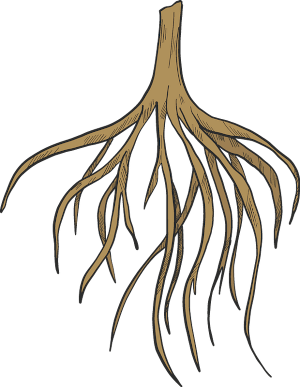
\includegraphics{root}
        \caption{rādīx, rādīcis (f)}
    \end{minipage}%
    \begin{minipage}[hbp]{0.5\linewidth}
        \centering
        
\includegraphics{fumus}
        \caption{fūmus, -ī (m)}
    \end{minipage}
\end{figure}

\vnum{17}Cumque ēdūxisset
eōs Moysēs in \mpp{occursus, -ūs (m) <}{occurere}occursum Deī dē locō castrōrum, stetērunt ad
\mpp{rādīx montis $\leftrightarrow$}{altissima pars montis}rādīcēs montis. 
\vnum{18}Tōtus autem mōns Sināī
\mpp{fūmāre:}{fumum mittere}fūmābat, eō quod dēscendisset Dominus super eum in igne:
et ascenderet fūmus ex eō quasi dē \mimg{furnus}{fornax, fornācis (f)}fornāce,
eratque omnis mōns terribilis. 
\vnum{19}Et \mpp{sonitus, -ūs (m):}{sonus magnus, strepitus}sonitus buccinæ
\mpp{paulātim:}{tardē plus et plus et plus vel magis et magis et magis}paulātim crēscēbat in maius, et \mpp{prōlixus/a/um:}{longus}prōlixius
tendēbātur: Moysēs loquēbātur, et Deus respondēbat eī. 
\vnum{20}Dēscenditque
Dominus super montem Sināī in ipsō montis \mpp{vertex, verticis
(m):}{altissima pars}vertice, et vocāvit Moysen in
\mpp{cacūmen, cacūminis (m):}{altissima pars}cacūmen eius.

Quō cum ascendisset, 
\vnum{21}dīxit ad eum:
``Dēscende, et \mpp{contestāre populum:}{fac tē testem verbōrum meōrum populō; narra populō ea quae tibi dixī}contestāre populum: nē forte velit
\mpp{trānscendere:}{transīre}trānscendere terminōs ad videndum Dominum, et
pereat ex eīs plūrima multitūdō. 
\vnum{22}Sacerdōtēs quoque quī accēdunt ad
Dominum, sānctificentur, nē percutiat eōs.''

\vnum{23}Dīxitque Moysēs ad Dominum:
``Nōn poterit \mpp{vulgus, -ī (n):}{multitudo, turba}vulgus ascendere in
montem Sināī: tū enim \mpp{testificārī:}{testis esse}testificātus es, et iussistī, dīcēns:
Pōne \mpp{terminus, -ī (m):}{res quae indicat finis reī, e.g: lapis positus inter agrōs}terminōs circā montem, et sānctificā illum.''

\vnum{24}Cui ait Dominus:
``Vāde, dēscende: as\-cendēsque tū, et Aarōn tēcum: sacerdōtēs autem et
populus nē trānseant terminōs, nec ascendant ad Dominum, nē forte
interficiat illōs.''

\vnum{25}Dēscenditque Moysēs ad populum, et omnia nārrāvit
eīs.

\chapter{}

\titleimg{tcorth}

\mktitle{Capitulum Vicesimum}
\thispagestyle{empty}

\cstart{L}{ocūtusque} est Dominus cūnctōs sermōnēs hōs: 

\vnum{2}``Ego sum Dominus Deus
tuus, quī ēdūxī tē dē terrā Ægyptī, dē domō servitūtis.  \vnum{3}Nōn habēbis deōs
aliēnōs cōram mē. \vnum{4}Nōn faciēs tibi \mpp{sculptile, -is (n):}{rēs secandō facta ut videatur alicuī reī similis, e.g: signum}sculptile, neque omnem
\mpp{similitūdō, -inis (f):}{rēs quae formam aliae reī similem habet; imāgō}similitūdinem quæ est in cælō \mpp{dēsuper:}{ē locō altiore}dēsuper, et
quæ in terrā deorsum, nec eōrum quæ sunt in aquīs sub terrā. 
\vnum{5}Nōn adōrābis
ea, neque cōlēs: ego sum Dominus Deus tuus fortis,
\mpp{zēlōtēs, -ae (m):}{qui amat aliquem et non vult eum aliquem amāre}zēlōtēs, \mpp{vīsitāre:}{vīsum īre}vīsitāns
\mpp{inīquitās, -ātis (f):}{rēs mala ab homine facta; mala anima propter rem malam factam}inīquitātem patrum in fīliōs, in tertiam et quārtam
\mpp{generātio, -ōnis (f):}{e.g una generatio parentibus constat, līberīs
eōrum altera generatio constat, etc...}generātiōnem eōrum quī ōdērunt mē:
\vnum{6}et faciēns \mpp{misericordia, -ae (f):}{quod sentimus dum vidēmus alium
patī}misericordiam in mīllia hīs quī dīligunt mē, et cūstōdiunt
\mpp{praeceptum, -ī:}{quod praecipitur}præcepta mea.''

\vnum{7}``Nōn \mpp{assumere:}{ad mē sumere; aliquem sibi adiungere ad fīnem aliquem capiendum}assūmēs nōmen
Dominī Deī tuī in \mpp{in vānum:}{frūstrā}vānum: nec enim habēbit
\mpp{īnsons, īnsontis (adj):}{quī rem malam nōn fēcit}īnsontem Dominus eum quī assūmpserit nōmen Dominī Deī suī
frūstrā.'' 

\vnum{8}\mpp{mementō:}{memoriā tene}``Mementō ut diem \mpp{sabbatum, -ī (n):}{dies
septimus quō non licet hominibus laborāre}sabbatī
\mpp{sānctificāre:}{sanctum facere}sānctificēs. 
\vnum{9}Sex diēbus operāberis, et
faciēs omnia opera tua. 
\vnum{10}Septimō autem diē sabbatum Dominī Deī tuī est:
nōn faciēs omne opus in eō, tū, et fīlius tuus et fīlia tua, servus tuus et
ancilla tua, \mpp{iūmentum, -ī (n):}{animal utile ad gerendum vel trahendum
e.g, equī, bovēs, et cetera}iūmentum tuum, et advena quī est intrā portās
tuās. 
\vnum{11}Sex enim diēbus fēcit Dominus cælum et terram, et mare, et omnia
quæ in eīs sunt, et requiēvit in diē septimō: \mpp{idcircō:}{proptereā,
ideō}idcircō \mpp{benedīcere:}{sanctum facere}benedīxit Dominus diēī
sabbatī, et sānctificāvit eum.''

\vnum{12}\mpp{honōrāre:}{colere aliquem propter eius virtutēs vel rēs bene factās}``Honōra patrem tuum et
mātrem tuam, ut sīs \mpp{longævus/a/um:}{senex}longævus super terram, quam Dominus
Deus tuus dabit tibi.''

\vnum{13}``Nōn occīdēs.''

\vnum{14}``Nōn \mpp{mœchārī:}{iacēre in lectō cum uxore vel marītō alius}mœchāberis.''

\vnum{15}``Nōn \mpp{fūrtum, -ī (n):}{e.g, si capis pecuniam vel aliquid alius, hoc est furtum}fūrtum faciēs.''

\vnum{16}``Nōn loqueris contrā proximum tuum falsum \mpp{testimōnium, -ī (n):}{id quod ā teste dīcitur}testimōnium.''

\vnum{17}``Nōn \mpp{concupiscere:}{valdē cupere}concupīscēs domum
proximī tuī, nec dēsīderābis uxōrem eius, nōn servum, nōn ancillam, nōn
bovem, nōn asinum, nec omnia quæ illīus sunt.''

\begin{figure}[hp]
    \begin{minipage}[hbp]{0.5\linewidth}
        \centering
        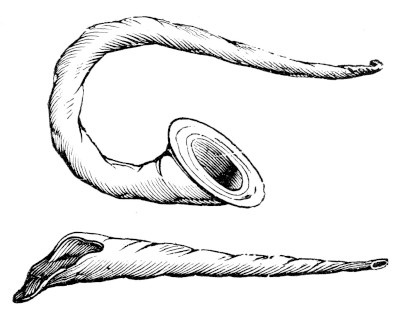
\includegraphics{bucina}
        \caption{buccina, -ae (f)}
    \end{minipage}%
    \begin{minipage}[hbp]{0.5\linewidth}
        \centering
        
\includegraphics{fumus}
        \caption{fūmus, -ī (m)}
    \end{minipage}
\end{figure}

\vnum{18}Cūnctus autem populus
vidēbat vōcēs et \mpp{lampas, lampadis (f):}{ignis}lampadēs, et \mpp{sonitus, -ūs (m):}{sonus
magnus, strepitus}sonitum buccinæ, montemque
\mpp{fūmāre:}{fūmum mittere}fūmantem: et perterritī ac \mpp{pavor, -ōris
(m):}{timor}pavōre \mpp{concussus/a/um:}{pulsātus; turbātus}concussī, stetērunt procul, 
\vnum{19}dīcentēs
Moȳsī: ``Loquere tū nōbīs, et audiēmus: nōn loquātur nōbīs Dominus, nē
forte moriāmur.'' 

\vnum{20}Et ait Moysēs ad populum: ``Nōlīte timēre: ut
enim probāret vōs vēnit Deus, et ut \mpp{terror, -ōris (m):}{magnus timor}terror illīus
esset in vōbīs, et nōn \mpp{peccātum, -ī:}{res contra legem
acta}peccārētis.''

\vnum{21}Stetitque populus dē longē. Moysēs autem accessit ad
\mpp{cālīgō, cālīginis (f):}{aer per quem difficile est vidēre}cālīginem in quā erat Deus. 

\vnum{22}Dīxit prætereā Dominus ad
Moysēn: ``Hæc dīcēs fīliīs Isrāēl: Vōs
vīdistis quod dē cælō locūtus sim vōbīs. 
\vnum{23}Nōn faciētis deōs argenteōs,
nec deōs aureōs faciētis vōbīs. 
\vnum{24}Altāre dē terrā faciētis mihi, et
offerētis super eō \mpp{holocaustum, -ī (n):}{sacrificium igne factum}holocausta et
\mpp{pācificus/a/um:}{pacem faciens}\mpp{pācificum (sacrificium):}{sacrificium in quō parva pars sacrificii Deō datur et magna pars populō}pācifica vestra, ovēs vestrās et bovēs
in omnī locō in quō memoria fuerit nōminis meī: veniam ad tē, et
\mpp{benedīcere:}{sanctum facere}benedīcam tibi. 
\vnum{25}Quod sī altāre \mimg{rock}{lapis, lapidis (m)}\mpp{lapideus/a/um:}{ex lapidibus factum}lapideum
fēcerīs mihi, nōn ædificābis illud dē sectīs lapidibus: sī
enim levāverīs cultrum super eō, \mpp{polluere:}{foedum facere}polluētur. 
\vnum{26}Nōn ascendēs
per gradūs ad altāre meum, nē \mpp{revēlāre:}{efficere ut aliquid occultum appāreat}revēlētur
\mpp{turpitūdō, -inis (f) <}{turpis}turpitūdō tua.''

\invisiblechapter{Cap. XXI-XXIV}

\titleimg{sinai}

\mktitle{Capitula ā Vīcēsimō Prīmō}
\vspace*{-1.4cm}
\mktitle{ad Vīcēsimum Quartum}
\thispagestyle{empty}

[Permultae Deī lēgēs in capitulīs ā vīcēsimō prīmō ad vīcēsimum tertium
continentur. Multae sunt lēgēs dē iniūriīs: e.g, ``Quī percusserit patrem
suum aut mātrem, morte moriātur.''

Multae sunt lēgēs dē agrīs et animālium
gregibus: e.g, ``Sī occurrerīs bovī inimīcī tuī, aut asinō errantī, redūc
ad eum.''

Multae sunt lēgēs dē Deō colendō: e.g, \mpp{prīmitiae, -ārum (f):}{primae rēs quae ex agrīs metuntur}``Prīmitiās frūgum terræ
tuæ \mpp{dēferre:}{ferre aliquid aliquō}dēferēs in domum Dominī Deī tuī.''

Hīc incipit
capitulum vīcēsimum\linebreak quārtum:]

\mimg{root}{rādīx, rādīcis (f)}\vnum{1}[Deus] Moȳsī quoque dīxit: ``Ascende ad Dominum
tū, et Aarōn, Nadab et Abiu, et septuāgintā senēs ex
Isrāēl, et adōrābitis procul.
\vnum{2}Solusque
Moysēs ascendet ad Dominum, et illī nōn appropinquābunt:
nec populus ascendet cum eō.''

\vnum{3}Venit ergō Moysēs et nārrāvit
\mpp{plēbs, plēbis}{populī multitudo}plēbī omnia verba Dominī, atque
\mimg{judge_small}{iudex, iudicis (m/f)}\mpp{iūdicium, -ī:}{quod iudex tradit}iūdicia:
responditque omnis populus ūnā vōce: ``Omnia verba Dominī, quæ locūtus est,
faciēmus.''

\vnum{4}Scrīpsit autem Moysēs ūniversōs sermōnēs Dominī: et manē
\mpp{cōnsurgere:}{surgere}cōnsurgēns, ædificāvit altāre ad
\mpp{rādīx montis $\leftrightarrow$}{altissima pars montis}rādīcēs montis,
et duodecim \mpp{titulus, -ī (m):}{columna}titulōs per duodecim tribus
Isrāēl. 

\vnum{5}Mīsitque iuvenēs dē fīliīs Isrāēl, et obtulērunt
\mpp{holocaustum, -ī (n):}{sacrificium igne factum}holocausta,
\mpp{immolāre:}{sacrificium facere}immolāvēruntque \mpp{victima, -ae
(f):}{animal sacrificiō statutum}victimās \mpp{pācificus/a/um:}{pacem
faciens}pācificās Dominō, \mpp{vitulus, -ī (m):}{bōs parvus}vitulōs.  
\vnum{6}Tulit itaque Moysēs
dīmidiam partem sanguinis, et mīsit in \mimg{crater}{crātēr, crātēris (m)}crātērās: partem
autem \mpp{residuus/a/um:}{quod reliquum est}residuam fūdit super altāre. 

\vnum{7}Assūmēnsque \mpp{volūmen, volūminis (n):}{liber}volūmen fœderis, legit audiente populō: quī
dīxērunt: ``Omnia quæ locūtus est Dominus, faciēmus, et erimus
\mpp{obēdiēns, -entis (adj):}{parēns}obēdientēs.''

\vnum{8}Ille vērō sūmptum sanguinem
\mpp{respergere:}{aspergere}respersit in populum, et ait: ``Hic est sanguis fœderis quod
\mpp{pangō, pangere, pepigī, pactum:}{constituere}pepigit Dominus vōbīscum super cūnctīs sermōnibus hīs.''

\vnum{9}Ascendēruntque Moysēs et Aarōn, Nadab et Abiu, et septuāgintā dē seniōribus
Isrāēl: 
\vnum{10}et vīdērunt Deum Isrāēl: et sub pedibus eius quasi opus
\mimg{rock}{lapis, lapidis (m)}lapidis \mimg{bluegem}{sapphīrus, -ī (m)}\mpp{sapphīrinus/a/um <}{sapphīrus}sapphīrinī, et quasi cælum, cum serēnum est. 
\vnum{11}Nec
super eōs quī procul recesserant dē fīliīs Isrāēl, mīsit manum suam,
vīdēruntque Deum, et \mpp{comedere:}{totum ēsse; ēsse}comēdērunt, ac
bibērunt. 

\vnum{12}Dīxit autem Dominus ad Moysēn: ``As\-cende ad mē
in montem, et estō ibi: dabōque tibi tabulās \mpp{lapideus/a/um:}{ex
lapidibus factum}lapideās, et lēgem, ac \mpp{mandātum, -ī (n):}{id quod
imperatum vel traditum est}mandāta quæ scrīpsī ut doceās eōs.''

\vnum{13}Surrēxērunt Moysēs et Iōsve minister eius: ascendēnsque Moysēs in montem
Deī, 
\vnum{14}seniōribus ait: ``\mpp{expectāre =}{exspectāre}Expectātē hīc dōnec revertāmur ad
vōs. Habētis Aarōn et Hur vōbīscum: sī quid nātum fuerit
\mpp{quaestiō, -ōnis (f):}{quod interrogatur, praecipuē cum respondēre difficile est: e.g, ``Estne Deus?'', ``Quid est hominibus bonum?'', etc.}quæstiōnis, referētis ad eōs.''

\vnum{15}Cumque ascendisset Moysēs,
operuit\linebreak nūbēs montem, 
\vnum{16}et habitāvit glōria Dominī super Sinaī, tegēns
illum nūbe sex diēbus: septimō autem diē vocāvit eum dē mediō
\mpp{cālīgō, cālīginis (f):}{aer per quem difficile est vidēre}cālīginis. 
\vnum{17}Erat autem speciēs glōriæ Dominī quasi ignis
\mpp{ārdēre:}{habēre ignem in sē}ārdēns super \mpp{vertex, verticis
(m):}{altissima pars}verticem montis in cōnspectū fīliōrum Isrāēl. 
\vnum{18}\mpp{ingredī:}{intus īre}Ingressusque Moysēs medium \mpp{nebula, -ae (f):}{nūbēs prope terram}nebulæ,
ascendit in montem: et fuit ibi quadrāgintā diēbus, et quadrāgintā
noctibus.

\chapter{}

\titleimg{goldencalf}

\mktitle{Capitula ā Vicesimō Quīntō}
\vspace*{-1.4cm}
\mktitle{ad Trīcēsimum Secundum}
\thispagestyle{empty}

[Hīs in capitulīs, Deus cōnsilium tabernāculī sibi cōnficiendī dat, 
dīcēns ``Facientque mihi \mpp{sānctuārium, -ī (n):}{sacer locus}sānctuārium,
et habitābō in mediō eōrum.'' Dē eius māteriīs et ōrnāmentīs loquitur. 
Legēs Deī illīc in \mpp{????}{????}arcā pōnentur.

Etiam Deus vult nōnnūllōs virōs fierī sacerdōtēs: Aarōn, Nadab, Abiu, Eleazar, et Ithamar. Loquitur dē vestīmentīs eōrum.

Deinde imperat Deus sacrificia duōrum ovium cotīdiē esse facienda, et docet quōmodo hoc fierī dēbeat.

Tandem Deus ipse legēs scrībit et Moȳsī dat.

Hīc incipit capitulum trīcēsimum secundum:]


\vnum{1}Vidēns autem populus quod moram faceret dēscendendī dē monte
Moysēs, \mpp{congregāre:}{in unum locum cōgere vel ferre
vel ducere}congregātus adversus Aarōn, dīxit: ``Surge, fac nōbīs deōs, quī
nōs \mpp{praecēdere:}{ante īre}præcēdant: Moysī enim huic
virō, quī nōs ēdūxit dē terrā Ægyptī, ignōrāmus quid acciderit.''

\vnum{2}Dīxitque
ad eōs Aarōn: ``Tollite \mpp{inaurēs, inaurium (f. pl.):}{ornamenta in auribus posita}inaurēs aureās dē uxōrum,
fīliōrumque et fīliārum vestrārum auribus, et afferte ad mē.''

\vnum{3}Fēcitque
populus quæ iusserat, \mpp{dēferre:}{ferre aliquid aliquō}dēferēns inaurēs
ad Aarōn. 
\vnum{4}Quās cum ille accēpisset, fōrmāvit opere \mpp{fūsōrius/a/um:}{quod funditur}fūsōriō, et fēcit ex
eīs \mpp{vitulus, -ī (m):}{bōs parvus}vitulum \mpp{cōnflātilis, -e (adj):}{quod flandō factum est}cōnflātilem. Dīxēruntque: ``Hī
sunt dīī tuī Isrāēl, quī tē ēdūxērunt dē terrā Ægyptī.''

\vnum{5}Quod cum vīdisset Aarōn, ædificāvit altāre cōram eō, et
\mpp{præcō, præcōnis (m):}{quī magnā voce aliquid nuntiat}præcōnis vōce clāmāvit dīcēns: Crās \mpp{sōlemnitās, -ātis
(f):}{diēs quī certīs temporibus quotannis fit quō homines deum
serviunt}sōlemnitās Dominī est. 
\vnum{6}Surgentēsque māne, obtulērunt
\mpp{holocaustum, -ī (n):}{sacrificium igne factum}holocausta, et hostiās
\mpp{pācificus/a/um:}{pacem faciens}pācificās, et sēdit populus
\mpp{mandūcāre:}{cibum dentibus iterum iterumque premere}mandūcāre, et bibere, et surrēxērunt lūdere. 

\vnum{7}Locūtus est
autem Dominus ad Moysen, dīcēns: ``Vāde, dēscende:
\mpp{peccātum, -ī:}{res contra legem acta}peccāvit populus tuus, quem
ēdūxistī dē terrā Ægyptī. 
\vnum{8}Recessērunt cito dē viā, quam ostendistī eīs:
fēcēruntque sibi vitulum cōnflātilem, et adōrāvērunt, atque
\mpp{immolāre:}{sacrificium facere}immolantēs eī hostiās, dīxērunt: Istī
sunt dīī tuī Isrāēl, quī tē ēdūxērunt dē terrā Ægyptī.'' 

\vnum{9}\mpp{rūrsum =}{rūrsus}Rūrsumque ait Dominus ad Moysēn: ``Cernō quod populus iste
dūræ \mpp{cervīx, cervīcis (f):}{posterior pars collī; collum}cervīcis sit: 
\vnum{10}dīmitte mē, ut īrāscātur \mpp{furōr,
-ōris (m):}{qui habet `furōrem' in sē valde perturbatur}furor meus contrā
eōs, et dēleam eōs, faciamque tē in gentem magnam.'' 

\vnum{11}Moysēs autem ōrābat Dominum Deum suum, dīcēns: ``Cūr, Domine, īrāscitur furor tuus contrā
populum tuum, quem ēdūxistī dē terrā Ægyptī, in \mpp{fortitudō, -inis
(f):}{quod homo fortis habet}fortitūdine magnā, et in manū
\mpp{rōbustus/a/um:}{durus, valens}rōbustā? 
\vnum{12}Nē, \mpp{quæsō:}{homo dicit `quæsō' cum velit verba sua minus duriora viderī}quæsō, dīcant Ægyptiī: 
\mpp{callidus/a/um:}{doctus, praecipue rebus agendis, non rebus ex librīs}Callidē ēdūxit eōs,
ut interficeret in montibus, et dēlēret ē terrā: quiescat īra tua, et estō
\mpp{plācābilis, -e (adj):}{qui facile tranquillus fiērī potest}plācābilis
super \mpp{nēquitia, -ae (f):}{e.g, homo saepe mentitur: hoc est nēquitia eius. Homo saepe iratus est: hoc est nēquitia eius}nēquitiā populī tuī. 
\vnum{13}\mpp{recordor, -ārī, -ātus sum:}{meminisse}Recordāre Abraham, Isaac, et
Isrāēl servōrum tuōrum, quibus \mimg{iuro}{iurāre}iūrāstī per tēmetipsum,
dīcēns: \mpp{multiplicāre:}{multum facere; augēre}Multiplicābō sēmen
vestrum sīcut stēllās cælī; et ūniversam terram hanc, dē quā locūtus sum,
dabō sēminī vestrō, et possidēbitis eam semper.''

\vnum{14}Plācātusque est Dominus
nē faceret mālum quod locūtus fuerat adversus populum suum. 
\vnum{15}Et reversus
est Moysēs dē monte, portāns duās tabulās \mpp{testimōnium, -ī (n):}{id
quod ā teste dīcitur}testimōniī in manū suā, scrīptās ex utrāque parte, 
\vnum{16}et factās opere Deī: \mpp{scrīptūra, -ae (f):}{verba scrīpta}scrīptūra quoque Deī erat \mimg{pump}{rēs \emph{sculpta}}sculpta in
tabulīs. 
\vnum{17}Audiēns autem Iōsve tumultum populī \mpp{vociferārī:}{valde
exclamare}vōciferantis, dīxit ad Moysēn: ``Ululātus pugnæ audītur in
castrīs.'' 

\vnum{18}Quī respondit: ``Nōn est clāmor \mpp{adhortārī:}{hortārī}adhortantium ad
pugnam, neque \mpp{vōciferātiō, -ōnis (f):}{clamor}vōciferātiō \mpp{compellere:}{vī facere ut aliquis aliquid agat}compellentium ad
fugam: sed vōcem cantantium ego audiō.''

\vnum{19}Cumque appropinquāsset ad
castra, vīdit vitulum, et \mpp{chorus, -ī (m):}{actus corporis movendi
propter hominem cantantem vel similem}chorōs: īrātusque valdē, prōiēcit dē
manū tabulās, et \mpp{cōnfringere:}{ūnā frangere}cōnfrēgit eās ad
rādīcem montis: 
\vnum{20}\mpp{arripere:}{vī
prehendere}arripiēnsque vitulum quem fēcerant, \mpp{comburō, comburere, combussī, combussum:}{accendere}combussit,
et \mpp{conterō, conterere, contrīvī, contrītum:}{perdere}contrīvit usque
ad \mpp{pulvis, pulveris (m):}{terra minima et non umida}pulverem, quem sparsit
\mimg{root}{rādīx, rādīcis (f)}in aquam, et dedit ex eō pōtum fīliīs Isrāēl. 

\vnum{21}Dīxitque ad Aarōn: ``Quid
tibi fēcit hic populus, ut indūcerēs super eum peccātum maximum?''

\vnum{22}Cui
ille respondit: ``Nē \mpp{indignārī:}{aliquid graviter animō ferre; ferre non posse}indignētur dominus meus: tū enim nōstī
populum istum, quod prōnus sit ad mālum. 
\vnum{23}Dīxērunt mihi: Fac nōbīs
deōs, quī nōs præcēdant: huic enim Moȳsī, quī nōs ēdūxit dē terrā Ægyptī,
nescīmus quid acciderit. 
\vnum{24}Quibus ego dīxī: Quis vestrum habet aurum?
Tulērunt, et dedērunt mihi: et prōiēcī illud in ignem, ēgressusque est hic
\mpp{vitulus, -ī (m):}{bōs parvus}vitulus.'' 

\vnum{25}Vidēns ergō Moysēs populum
quod esset nūdātus (spoliāverat enim eum Aarōn propter
\mpp{ignōminia, -ae (f):}{id quod minime decet}\mpp{ignōminia sordis:}{id est, vitulus a populō factus}ignōminiam sordis, et inter hostēs nūdum cōnstituerat), 
\vnum{26}et stāns in portā castrōrum, ait: ``Sī quis est Dominī, iungātur mihi.''

Congregātīque sunt ad eum omnēs fīliī Levī 
\vnum{27}quibus ait: ``Hæc dīcit
Dominus Deus Isrāēl: Pōnat vir gladium super \mimg{femur}{femur, femoris/feminis (n)}femur suum. Īte, et reditē
dē portā usque ad portam per medium castrōrum, et occīdat ūnusquisque
frātrem, et amīcum, et proximum suum.''

\vnum{28}Fēcēruntque fīliī Levī iuxtā
sermōnem Moȳsī, cecidēruntque in diē illa quasi vīgintī tria mīllia
hominum. 

\vnum{29}Et ait Moysēs: ``\mpp{cōnsecrāre:}{sacrum facere}Cōnsecrāstis
manūs vestrās hodiē Dominō, \mpp{ūnusquisque:}{singulī hominēs}ūnusquisque in fīliō, et in frātre suō, ut
dētur vōbīs \mpp{benedictiō, -ōnis (f) <}{benedicere: sanctum facere}benedictiō.''

\vnum{30}Factō autem alterō diē, locūtus
est Moysēs ad populum: ``\mpp{peccāre:}{contra legem agere}Peccāstis \mpp{peccatum, -i (n):}{res contra legem acta}peccātum maximum: ascendam ad Dominum,
sī quōmodo quīverō eum \mpp{dēprecārī:}{aliquem aut aliquid per preces
a periculo liberare}dēprecārī prō scelere vestrō.''

\vnum{31}Reversusque ad
Dominum, ait: ``\mpp{obsecrāre:}{orāre, precārī}Obsecrō, peccāvit populus
iste peccātum maximum, fēcēruntque sibi deōs aureōs: aut dīmitte eīs hanc
\mpp{noxa, -ae (f):}{quod nocet}noxam, 
\vnum{32}aut sī nōn facis, dēlē mē dē librō tuō quem
scrīpsistī.'' 

\vnum{33}Cui respondit Dominus: ``Quī peccāverit mihi, dēlēbō eum dē
librō meō: 
\vnum{34}tū autem vāde, et dūc populum istum quō locūtus sum tibi:
\mpp{angelus, -ī (m):}{res viva, sapiens, et potēns ā Deō missa quae agit
quidquid Deus vult}angelus meus præcēdet tē. Ego autem in diē
\mpp{ulciscī:}{e.g, Agricola pastorem necat, deinde amicus pastoris agricolam necat, id est, amicus pastoris `ulciscitur' agricolam.}\mpp{ultiō, -ōnis (f) <}{ulciscī}ultiōnis \mpp{vīsitāre:}{vīsum īre}vīsitābō et hoc peccātum
eōrum.''

\vnum{35}Percussit ergō Dominus populum prō \mpp{reātus, -ūs (m):}{peccatum propter quod homo puniendus est}reātū vitulī,
quem fēcerat Aarōn. 


\chapter{}

\titleimg{tcorth}

\mktitle{Capitulum Tricesimum Tertium}
\thispagestyle{empty}

\cstart{L}{ocūtusque} est Dominus ad Moysen, dīcēns: ``Vāde, ascende
dē locō istō tū, et populus tuus quem ēdūxistī dē terrā Ægyptī, in terram
quam \mimg{iuro}{iurāre}iūrāvī Abraham, Isaac et Iācōb, dīcēns:
Sēminī tuō dabō eam: 
\vnum{2}et mittam \mpp{præcursor, -ōris (m)}{qui currit prae aliīs}præcursōrem tuī
\mpp{angelus, -ī (m):}{res viva, sapiens, et potēns ā Deō missa quae agit
quidquid Deus vult}angelum, ut ēiciam Chananæum, et
Amorrhæum, et Hethæum, et Pherezæum, et Hevæum, et Iebusæum, 
\vnum{3}et intrēs in
terram fluentem lacte et melle. Nōn enim ascendam tēcum, quia populus dūræ
\mpp{cervīx, cervīcis (f):}{posterior pars collī; collum}cervīcis es: nē
forte \mpp{disperdere:}{valde perdere}disperdam tē in viā.''

\vnum{4}Audiēnsque
populus sermōnem hunc pessimum, \mpp{lūgeō, lugēre, lūxī, luctum}{}lūxit: et nūllus ex mōre indūtus est cultū
suō. 

\vnum{5}Dīxitque Dominus ad Moysēn: ``Loquere fīliīs Isrāēl:
Populus dūræ cervīcis es: semel ascendam in mediō tuī, et dēlēbō tē. Iam
nunc dēpōne ōrnātum tuum, ut sciam quid faciam tibi.''

\begin{figure}[h!]
    \begin{minipage}[hp]{0.5\linewidth}
        \centering
        \includegraphics{tab2}
        \caption{tabernaculum, -ī (n)}
    \end{minipage}%
    \begin{minipage}[hp]{0.5\linewidth}
        \centering
        
\includegraphics{papilio}
        \caption{pāpiliō, -ōnis (m)}
    \end{minipage}
\end{figure}

\vnum{6}Dēposuērunt ergō
fīliī Isrāēl ōrnātum suum ā monte Horeb. 
\vnum{7}Moysēs quoque tollēns tabernāculum,
tetendit extrā castra procul, vocāvitque nōmen eius `Tabernāculum fœderis.'
Et omnis populus, quī habēbat aliquam \mpp{quaestiō, -ōnis (f):}{quod
interrogatur, praecipuē cum respondēre difficile est e.g, ``Estne Deus?'',
``Quid est hominibus bonum?'', etc.}quæstiōnem, ēgrediēbātur ad
tabernāculum fœderis, extrā castra. 
\vnum{8}Cumque ēgrederētur Moysēs ad
tabernāculum, surgēbat ūniversa \mpp{plēbs, plēbis (f):}{populī
multitudo}plēbs, et stābat ūnusquisque in ōstiō \mpp{pāpiliō, -ōnis (m):}{tabernaculum quod formam animalis eodem nomine habet}pāpiliōnis
suī, aspiciēbantque tergum Moȳsī, dōnec \mpp{ingredī:}{intus
īre}ingrederētur \mpp{tentōrium, -ī (n):}{tabernaculum}tentōrium. 

\vnum{9}Ingressō autem illō
tabernāculum fœderis, dēscendēbat columna nūbis, et stābat ad ōstium,
loquēbāturque cum Moyse, 
\vnum{10}cernentibus ūniversīs quod
columna nūbis stāret ad ōstium tabernāculī. Stābantque
ipsī, et adōrābant per forēs tabernāculōrum suōrum. 
\vnum{11}Loquēbātur autem Dominus ad Moysēn faciē ad faciem, sīcut solet loquī homō
ad amīcum suum. Cumque ille reverterētur in castra, minister eius Iosve
fīlius Nun, puer, nōn recēdēbat dē
tabernāculō. 

\vnum{12}Dīxit autem Moysēs ad Dominum:
``\mpp{praecipere:}{imperāre}Præcipis ut ēdūcam populum istum: et nōn
\mpp{indicāre:}{mōnstrāre}indicās mihi quem missūrus es mēcum,
\mpp{praesertim:}{praecipue}præsertim cum dīxerīs: Nōvī tē ex nōmine, et
invēnistī grātiam cōram mē. 
\vnum{13}Sī ergō invēnī grātiam in cōnspectū tuō,
ostende mihi faciem tuam, ut sciam tē, et inveniam grātiam ante oculōs tuōs:
\mpp{respicere:}{aspicere iuvandī causā}respice populum tuum gentem hanc.''

\vnum{14}Dīxitque Dominus: ``Faciēs mea \mpp{praecēdere:}{ante īre}præcēdet tē, et
\mpp{requiēs, requiētis (f):}{tempus quō homo non laborat}requiem dabō tibi.''

\vnum{15}Et ait
Moysēs: ``Sī nōn tū ipse præcēdās, nē ēdūcās nōs dē locō istō. 
\vnum{16}In quō
enim scīre poterimus ego et populus tuus invēnisse nōs grātiam in cōnspectū
tuō, nisi ambulāverīs nōbīscum, ut \mpp{glōrificāre:}{gloriosum
facere}glōrificēmur ab omnibus populīs quī habitant super terram?''

\vnum{17}Dīxit
autem Dominus ad Moysēn: ``Et verbum istud, quod locūtus es, faciam:
invēnistī enim grātiam cōram mē, et tēipsum nōvī ex nōmine.''

\vnum{18}Quī ait: ``Ostende mihi glōriam tuam.''

\vnum{19}Respondit: ``Ego ostendam omne bonum tibi, et
vocābō in nōmine Dominī cōram tē: et \mpp{miserērī:}{dolorem sentīre propter miserum alterum}miserēbor cui
voluerō, et clēmēns erō in quem mihi placuerit.''

\vnum{20}\mpp{rūrsum =}{rūrsus}Rūrsumque ait: ``Nōn poteris vidēre faciem meam: nōn enim
vidēbit mē homō et vīvet.'' 

\vnum{21}Et iterum: ``Ecce, inquit, est locus apud mē,
et stābis suprā \mimg{hole}{forāmen, forāminis (n)}\mpp{petra, -ae (f):}{lapis}petram.
\vnum{22}Cumque trānsībit
glōria mea, pōnam tē in forāmine petræ, et
\mpp{prōtegere:}{defendere}prōtegam dexterā meā, dōnec trānseam: 
\vnum{23}tollamque manum
meam, et vidēbis posteriōra mea: faciem autem meam vidēre nōn poteris.''

\chapter{}

\titleimg{tcorth}

\mktitle{Ad Finem}
\thispagestyle{empty}

[Hīc incipit capitulum trīcēsimum quārtum:]

\vnum{1}Ac \mpp{deinceps:}{deinde}deinceps:
``\mpp{præcīdere:}{frangere in partes}Præcīde,'' ait, ``tibi duās tabulās \mpp{lapideus/a/um:}{ex
lapidibus factum}lapideās \mpp{īnstar + gen:}{similis}īnstar priōrum, et
scrībam super eās verba, quæ habuērunt tabulæ quās frēgistī. 
\vnum{2}Estō parātus
manē, ut ascendās statim in montem Sināī, stābisque mēcum super
\mpp{vertex, verticis (m):}{altissima pars}verticem montis. 
\vnum{3}Nūllus
ascendat tēcum, nec videātur \mpp{quispiam =}{aliquis}quispiam per tōtum montem:
bovēs quoque et ovēs nōn pāscantur ē contrā.''

\vnum{4}\mpp{excidere:}{secare partem alicuis et capere illam partem}Excidit ergō
duās tabulās lapideās, quālēs anteā fuerant: et dē nocte
\mpp{cōnsurgere:}{surgere}cōnsurgēns ascendit in montem Sināī, sīcut
\mpp{praecipere:}{imperāre}præcēperat eī Dominus, portāns sēcum tabulās. 
\vnum{5}Cumque dēscendisset Dominus per nūbem, stetit Moysēs cum
eō, invocāns nōmen Dominī. 

\vnum{6}Quō trānseunte cōram eō, ait: \mpp{dominātor, -ōris (m):}{qui dominus est multārum rērum}``Dominātor
Domine Deus, \mpp{misericors, -cordis (adj):}{qui facile dolorem sentit
propter aliquem miserum; clemens}misericors et clēmēns, patiēns et multæ
\mpp{miserātiō, -ōnis (f) <}{miser}miserātiōnis, ac \mpp{vērāx, vērācis
(adj):}{qui vera dicit}vērāx, 
\vnum{7}quī cūstōdīs
\mpp{misericordia, -ae (f):}{quod sentimus dum vidēmus alium
patī}misericordiam in mīllia; quī aufers \mpp{inīquitās, -ātis (f):}{rēs
mala ab homine facta; mala anima propter rem malam factam}inīquitātem, et
scelera, atque \mpp{peccātum, -ī:}{res contra legem acta}peccāta, nūllusque
apud tē per sē \mpp{innocēns, -centis (adj):}{qui non nocet}innocēns est; quī reddis inīquitātem patrum
fīliīs, ac \mpp{nepos, nepōtis (m):}{filius filiī vel filia filiae}nepōtibus in tertiam et quārtam
\mpp{prōgeniēs, -ēī (f):}{filiī vel filiae alicuius, et filiī vel filiae
hōrum, et filiī vel filiae hōrum, etc.}prōgeniem.''

\vnum{8}\mpp{festīnus/a/um:}{celeriter aliquid
agens}Festīnusque Moysēs, \mpp{curvātus/a/um:}{quod non habet formam rectam}curvātus est prōnus in terram, et
adōrāns 
\vnum{9}ait: ``Sī invēnī grātiam in cōnspectū tuō, Domine,
\mpp{obsecrāre:}{orāre, precārī}obsecrō ut gradiāris nōbīscum (populus enim
dūræ \mpp{cervīx, cervīcis (f):}{posterior pars collī; collum}cervīcis est)
et auferās inīquitātēs nostrās atque peccāta, nōsque possideās.''

\vnum{10}Respondit Dominus: ``Ego inībō \mpp{pactum, -ī (n):}{quod inter aliquōs
convenit}pactum videntibus cūnctīs: signa faciam quæ numquam vīsa sunt
super terram, nec in ūllīs gentibus, ut cernat populus iste, in cuius es
mediō, opus Dominī terribile quod factūrus sum. 
\vnum{11}\mpp{observābitis
azȳma:}{quotannis diem sanctam celebrētis in quā azymī panēs
comeduntur}Observā cūncta quæ hodiē \mpp{mandāre:}{tradere}mandō tibi...''

[Deus plūrēs lēgēs Moȳsī dat.] 

\vnum{27}Dīxitque Dominus ad
Moysēn: ``Scrībe tibi verba hæc, quibus et tēcum et cum
Isrāēl \mpp{pangō, pangere, pepigisse, pactum:}{constituere, statuere}pepigī fœdus.''

\vnum{28}Fuit ergō ibi cum
Dominō quadrāgintā diēs et quadrāgintā noctēs: pānem nōn comēdit, et aquam
nōn bibit, et scrīpsit in tabulīs verba fœderis decem. 
\vnum{29}Cumque
dēscenderet Moysēs dē monte Sināī, tenēbat duās tabulās \mpp{testimōnium,
-ī (n):}{id quod ā teste dīcitur}testimōniī, et ignōrābat quod
\mpp{cornūtus/a/um:}{cornua habens}cornūta esset faciēs sua ex
\mpp{cōnsortiō, -ōnis (f):}{congregatiō}cōnsortiō
sermōnis Dominī. 
\vnum{30}Videntēs autem Aarōn et fīliī Isrāēl
cornūtam Moȳsī faciem, timuērunt prope accēdere. 
\vnum{31}Vocātīque ab eō, reversī sunt tam Aarōn, quam prīncipēs
\mpp{synagōga, -ae (f):}{grex hominum}synagōgæ. Et postquam locūtus est ad eōs, 
\vnum{32}vēnērunt ad
eum etiam omnēs fīliī Isrāēl: quibus præcēpit cūncta quæ audierat ā Dominō
in monte Sināī. 
\vnum{33}Implētīsque sermōnibus, posuit \mpp{vēlāmen, vēlaminis (n):}{vestis quae faciem operit}vēlāmen
super faciem suam. 
\vnum{34}Quod \mpp{ingredī:}{intus īre}ingressus ad Dominum,
et loquēns cum eō, auferēbat dōnec exīret, et tunc loquēbātur ad fīliōs
Isrāēl omnia quæ sibi fuerant imperāta. 
\vnum{35}Quī vidēbant faciem ēgredientis
Moȳsī esse cornūtam, sed operiēbat ille rūrsus faciem suam,
\mpp{sīquandō:}{sī aliquando}sīquandō loquēbātur ad eōs.

[Moysēs lēgēs Deī populō dat,
deinde pergit populus \mimg{tab2}{tabernaculum, -ī (n)}tabernāculum Deī cōnficere.
Tabernāculō perfectō, nūbēs (Deus) tabernāculum operuit.]

[Capitulum Quadrāgēsimum:]

\vnum{34}Sīquandō nūbēs tabernāculum dēserēbat,
proficīscēbantur fīliī Isrāēl per \mpp{turma, -ae (f):}{multitūdō}turmās
suās: 
\vnum{35}Sī pendēbat \mpp{dēsuper:}{ē locō altiore}dēsuper, manēbant in
eōdem locō. 
\vnum{36}Nūbēs \mpp{quippe =}{certe}quippe Dominī
\mpp{incubāre:}{super aliquem rem cubāre, requiescere}incubābat per diem tabernāculō, et ignis in nocte,
videntibus cūnctīs populīs Isrāēl per cūnctās \mpp{mānsiō, -ōnis
(f):}{locus ubi iter facientes noctu manent}mānsiōnēs suās.

[Fīnis Librī Exodī] 


\chapter{}
% \newgeometry{top=0.75in, bottom=1.0in, outer=1.75in, inner=0.4in, heightrounded, 
% marginparwidth=3.5cm, marginparsep=0.5cm}

\newgeometry{top=0.75in, bottom=3cm, outer=3cm, inner=3cm}

\pagestyle{fancy}
\fancyhead{}
\chead{}
%\rhead{\thechapter}
\cfoot{} % get rid of the page number
\renewcommand{\headrulewidth}{1pt}
\renewcommand{\footrulewidth}{0pt}
{\tiny
    \begin{flushleft}
    \twocolumn
    \parskip 0.5ex
    \setlength{\parindent}{0pt}
    \input{lexicon.tex}
    \end{flushleft}
}

\end{document}
